

%% ==== Liste des abréviations et sigles ====
\chapter*{Liste des abréviations et sigles}
\addcontentsline{toc}{chapter}{Liste des abréviations et sigles}
\begin{description}
\item[EM] Espérance-Maximisation (Expectation-Maximization)
\item[GMM] Modèle de Mélange Gaussien (Gaussian Mixture Model)
\item[ELBO] Borne Inférieure de l'Évidence (Evidence Lower Bound)
\item[KL] Divergence de Kullback-Leibler
\item[VI] Inférence Variationnelle (Variational Inference)
\item[SVI] Inférence Variationnelle Stochastique (Stochastic Variational Inference)
\item[VAE] Auto-encodeur Variationnel (Variational Autoencoder)
\item[AEVB] Bayes Variationnel Auto-Encodant (Auto-Encoding Variational Bayes)
\item[SGVB] Estimateur Variationnel Bayésien par Gradient Stochastique (Stochastic Gradient Variational Bayes)
\item[CAVI] Montée par Coordonnées pour l'Inférence Variationnelle (Coordinate Ascent Variational Inference)
\item[MAP] Maximum A Posteriori
\item[MLE] Estimateur du Maximum de Vraisemblance (Maximum Likelihood Estimator)
\item[HMM] Modèle de Markov Caché (Hidden Markov Model)
\item[PPCA] Analyse en Composantes Principales Probabiliste
\item[LDA] Allocation de Dirichlet Latente (Latent Dirichlet Allocation)
\item[BIC] Critère d'Information Bayésien (Bayesian Information Criterion)
\item[AIC] Critère d'Information d'Akaike (Akaike Information Criterion)
\item[ICL] Critère de Vraisemblance Classifiante Intégrée
\item[SEM] EM Stochastique (Stochastic EM)
\item[GEM] EM Généralisé (Generalized EM)
\item[MCAR] Données Manquantes Complètement Aléatoires (Missing Completely At Random)
\item[MAR] Données Manquantes Aléatoires (Missing At Random)
\item[NLP] Traitement Automatique du Langage Naturel (Natural Language Processing)
\end{description}

%% ==== Introduction générale ====
\chapter*{Introduction générale}
\addcontentsline{toc}{chapter}{Introduction générale}
\markboth{INTRODUCTION GÉNÉRALE}{INTRODUCTION GÉNÉRALE}

\section*{Contexte et problématique}
Les modèles à variables latentes, au premier rang desquels les mélanges gaussiens, sont ajustés depuis plus de quarante ans par l'algorithme Espérance-Maximisation (EM) de Dempster, Laird et Rubin (1977). L'EM fournit un estimateur ponctuel du maximum de vraisemblance, exige que le nombre de composantes $K$ soit fixé à l'avance et peut converger vers des solutions dégénérées. L'EM variationnel, dans sa forme bayésienne (Attias, 2000 ; Bishop, 2006), place des lois a priori sur les paramètres, approche leur loi a posteriori par un champ moyen et élague les composantes superflues. La question traitée est la suivante : \emph{que gagne-t-on, et que perd-on, en passant de l'EM classique à l'EM variationnel, et sur quelles preuves ces gains et ces pertes reposent-ils ?}

La littérature présente volontiers l'EM variationnel comme un progrès. Ce mémoire adopte la position inverse du soupçon méthodique : chaque avantage (sélection automatique de $K$, incertitude, robustesse aux singularités, économie de calcul) et chaque inconvénient (coût, sensibilité aux priors, biais d'approximation, irréversibilité de l'élagage, dépendance à $K_{\max}$) est relié à une preuve : un théorème, une expérience répliquée, une expérience unique, ou la mention « non testé ».

\section*{Trois niveaux d'inférence}
La comparaison n'a de sens que si l'on distingue trois niveaux, rassemblés à la figure~\ref{fig:trois_niveaux} (chapitre 2). (1) L'\emph{EM classique} estime $\theta$ par un point (maximum de vraisemblance) avec $q(Z) = p(Z \mid X, \theta)$ exact. (2) L'\emph{EM variationnel à $\theta$ ponctuel} (Neal et Hinton, 1998 ; la LDA de Blei, Ng et Jordan, 2003) approche $q(Z)$ mais garde $\theta$ ponctuel. (3) Le \emph{Bayes variationnel} (VB) rend $\theta$ aléatoire et approche $q(\theta)$. Un comparateur intermédiaire, le \emph{MAP-EM}, ajoute les priors du VB à l'EM sans distribution sur $\theta$ : il isole l'effet de la régularisation de celui de l'inférence bayésienne complète.

\section*{Thèse défendue}
Le VB ne « bat » pas l'EM. Il déplace la sélection de $K$ vers le choix des hyperparamètres (et de $K_{\max}$), apporte une incertitude approchée, au prix d'un coût et d'une sensibilité aux priors. Les termes « supériorité », « changement de paradigme » et « dérivation originale » sont bannis de ce mémoire : l'équivalence de Neal et Hinton y est reprise comme une re-démonstration rigoureuse, non comme une contribution.

\section*{Hypothèses et critères}
Les hypothèses sont fixées avant l'analyse. Au chapitre 2, dix scénarios synthétiques (S1 à S10) testent le chevauchement, le déséquilibre des poids, la sous-estimation de $K$, les queues épaisses, la dimension, le petit effectif, les aberrations, la grille de $\alpha_0$ autour du seuil $d/2$ de Rousseau et Mengersen (2011), un plan factoriel sur les priors et la sensibilité au seuil d'activité, chacun avec au moins 30 réplications, un test apparié et un critère d'équivalence. Au chapitre 3, huit hypothèses H1 à H8 (sélection de $K$, qualité à $N$ complet, petit $N$, coût, hyperparamètres, couverture des intervalles de crédibilité, chevauchement, dimension) sont posées pour le cas principal avec leurs critères de décision (tableau~\ref{tab:climat_hypotheses}) ; la correction de Holm s'applique à l'ensemble des tests, et l'équivalence est une issue légitime.

\section*{Méthode et reproductibilité}
Tous les algorithmes sont écrits en PyTorch à partir des équations, avec un \emph{critère d'arrêt commun} (tolérance relative de $10^{-6}$ sur le critère total, plafond de 500 étapes M, figure~\ref{fig:boucle_arret}) : aucune comparaison n'est faite avec des critères d'arrêt différents. Les tableaux et les figures sont produits par le code avec des graines fixées ; aucun nombre des tableaux n'est saisi à la main, et le dépôt est archivé (annexe A).

\section*{Périmètre}
Le mémoire porte sur les mélanges gaussiens (et de Student pour la robustesse), le modèle de Markov caché et la LDA. Le cas principal est le climat du Cameroun (données WorldClim) ; le cas secondaire est le risque de marché du S\&P 500 ; une comparaison pLSA contre LDA porte sur un corpus réel. La vision, la bio-informatique et la recommandation font l'objet d'une revue de la littérature, sans expérience. Les mélanges de Dirichlet infinis, les méthodes MCMC et les familles variationnelles structurées sont hors périmètre.

\section*{Plan}
Le chapitre 1 pose les fondements (variables latentes, ELBO, KL, EM, EM variationnel) en distinguant les trois niveaux d'inférence. Le chapitre 2 compare théoriquement puis expérimentalement les deux approches, avec la baseline EM-BIC/ICL et le MAP-EM, et aboutit à la grille « axe $\times$ preuve » du tableau~\ref{tab:2_17}. Le chapitre 3 présente le cas climatique, le cas du S\&P 500, la comparaison pLSA contre LDA, une revue de littérature pour les autres domaines, l'implémentation et le guide de décision avec niveaux de preuve. La conclusion générale dresse le bilan et les limites.


%% ==== PARTIE 1 ====
\part{REVUE DE LA LITTÉRATURE : FONDEMENTS ET ÉTAT DE L'ART}

%% ==== CHAPITRE : FONDEMENTS THÉORIQUES ET ALGORITHMES EM ====
\chapter{FONDEMENTS THÉORIQUES ET ALGORITHMES EM}
Ce premier chapitre pose l'ensemble des bases théoriques nécessaires à la compréhension du reste de ce mémoire, puis présente en détail les deux algorithmes qui en constituent l'objet central : l'algorithme Espérance-Maximisation (EM) classique et sa généralisation bayésienne, l'EM variationnel. Nous commençons par définir la notion de modèle à variables latentes, avant d'introduire les outils mathématiques indispensables  la vraisemblance et sa maximisation, les distributions gaussiennes et le modèle de mélange gaussien, le cadre bayésien, l'inégalité de Jensen et la divergence de Kullback-Leibler. Ces éléments théoriques permettent ensuite de dérouler, de façon rigoureuse et progressive, la formulation mathématique complète de l'EM classique puis de l'EM variationnel, en insistant à chaque étape sur les propriétés de convergence, les variantes existantes, ainsi que les avantages et les limites de chacune des deux approches.

\section{Modèles à variables latentes}
\subsection{Définition formelle}
Un modèle probabiliste à variables latentes est défini par la donnée d'un espace d'observations et d'un espace de variables cachées, reliés par une loi jointe. Intuitivement, on peut se représenter une variable latente comme une cause non observée qui explique la structure des données observées : par exemple, la note obtenue par un étudiant à un examen (observée) dépend de son niveau réel de maîtrise de la matière (non observé directement). Formellement, pour une observation $x_{i}$, on écrit :

\begin{equation}
\begin{adjustbox}{max width=0.92\linewidth}$\displaystyle p(x_{i} | \theta ) = \int _\mathcal{Z} p(x_{i}{,} z_{i} | \theta ) dz_{i}$\end{adjustbox}
\tag{1.1}
\label{eq:1_1}
\end{equation}
L'objectif de l'inférence est d'estimer le paramètre $\theta $ à partir des seules observations \{$x_{i}$\}, les variables latentes $z_{i}$ n'étant jamais directement observées. La loi jointe se factorise selon le processus génératif du modèle :

\begin{equation}
\begin{adjustbox}{max width=0.92\linewidth}$\displaystyle p(X{,} Z | \theta ) = p(Z | \theta ) \times  p(X | Z{,} \theta ) = \prod _{i} p(z_{i} | \theta ) p(x_{i} | z_{i}{,} \theta )$\end{adjustbox}
\tag{1.2}
\label{eq:1_2}
\end{equation}
Cette factorisation traduit le processus génératif du modèle : on tire d'abord les variables latentes selon leur loi a priori, puis les observations conditionnellement à ces variables latentes.

\subsection{Taxonomie des variables latentes}
Les variables latentes se présentent sous différentes formes selon la nature du modèle considéré. On distingue en particulier :

\begin{itemize}
\item les variables latentes discrètes, comme les indicateurs d'appartenance à un groupe dans les modèles de mélange ;
\item les variables latentes continues, comme les coordonnées dans un espace de représentation réduit, dans les modèles factoriels ;
\item les variables latentes structurées, comme les séquences d'états cachés dans les modèles de Markov cachés.
\end{itemize}
La nature des variables latentes influence directement la traçabilité du calcul de la vraisemblance marginale et, par conséquent, la forme de l'algorithme EM applicable au modèle considéré.

\subsection{Exemples fondamentaux}
Les modèles à variables latentes sont omniprésents dans les applications de l'apprentissage automatique. Le tableau 1.1 présente les exemples les plus représentatifs, qui seront pour certains repris au chapitre 3 dans le cadre des applications pratiques.

\begin{table}[H]
\centering
\small
\setlength{\tabcolsep}{0.14cm}
\begin{tabular}{|>{\raggedright\arraybackslash}p{3.4cm}|>{\raggedright\arraybackslash}p{3.7cm}|>{\raggedright\arraybackslash}p{2.9cm}|>{\raggedright\arraybackslash}p{3.7cm}|}
\hline
\textbf{Modèle} & \textbf{Variables latentes} & \textbf{Paramètres} & \textbf{Application} \\
\hline
Mélange gaussien (GMM) & Appartenance à une composante $z_{i}$ $\in $ \{1..K\} & $\pi $, $\mu _{k}$, $\Sigma _{k}$ & Clustering, estimation de densité \\
\hline
Modèle de Markov caché (HMM) & Séquence d'états discrets & A, B, $\pi _{0}$ & Reconnaissance vocale \\
\hline
ACP probabiliste (PPCA) & Coordonnées latentes $z_{i}$ $\in $ $\mathbb{R}^{L}$ & W, $\sigma ^{2}$ & Réduction de dimension \\
\hline
Analyse factorielle & Facteurs latents & $\Lambda $, $\Psi $ & Psychologie, économie \\
\hline
LDA & Topics par document, mots par topic & $\alpha $, $\beta $ & Modélisation de sujets textuels \\
\hline
VAE & Code latent $z_{i}$ $\in $ $\mathbb{R}^{L}$ & $\theta enc$, $\theta dec$ & Génération d'images \\
\hline
IRT & Niveau de compétence $\theta _{i}$ & $a_{j}$, $b_{j}$ & Tests psychométriques \\
\hline
\end{tabular}
\caption{Exemples fondamentaux de modèles à variables latentes}
\label{tab:1_1}
\end{table}
\section{Vraisemblance et estimation}
\subsection{Vraisemblance complète et vraisemblance incomplète}
La distinction entre vraisemblance complète et vraisemblance incomplète est au cœur de la compréhension de l'algorithme EM. La log-vraisemblance complète est définie sur l'espace des données complètes, c'est-à-dire en incluant les variables latentes :

\begin{equation}
\begin{adjustbox}{max width=0.92\linewidth}$\displaystyle \ell c(\theta ) = \log  p(X{,} Z | \theta ) = \Sigma _{i} \log  p(x_{i}{,} z_{i} | \theta )$\end{adjustbox}
\tag{1.3}
\label{eq:1_3}
\end{equation}
Cette quantité est généralement facile à optimiser, car p(X, Z | $\theta $) se factorise de manière simple, conduisant souvent à des expressions analytiques fermées pour les estimateurs du maximum de vraisemblance. En revanche, la log-vraisemblance incomplète, définie sur les seules observations, s'écrit :

\begin{equation}
\begin{adjustbox}{max width=0.92\linewidth}$\displaystyle \ell (\theta ) = \log  p(X | \theta ) = \Sigma _{i} \log  \int  p(x_{i}{,} z_{i} | \theta ) dz_{i} = \Sigma _{i} \log  \Sigma _{k} p(x_{i}{,} z_{i} = k | \theta )$\end{adjustbox}
\tag{1.4}
\label{eq:1_4}
\end{equation}
L'opération de logarithme d'une somme (ou d'une intégrale) détruit la structure factorielle favorable de la vraisemblance complète, rendant l'optimisation directe de $\ell $($\theta $) généralement intractable sur le plan analytique. C'est précisément cette difficulté que l'algorithme EM contourne de manière élégante, en s'appuyant sur une borne inférieure de la vraisemblance incomplète  l'ELBO  que nous introduisons dès à présent.

\subsection{L'inégalité de Jensen et le principe de la borne inférieure}
L'inégalité de Jensen est un résultat fondamental de l'analyse convexe qui sous-tend directement la construction de l'algorithme EM. Elle énonce que pour toute fonction concave f et toute variable aléatoire X, on a :

\begin{equation}
\begin{adjustbox}{max width=0.92\linewidth}$\displaystyle f(\mathbb{E}[X]) \geq  \mathbb{E}[f(X)]$\end{adjustbox}
\tag{1.5}
\label{eq:1_5}
\end{equation}
avec égalité si et seulement si X est constante presque sûrement, ou si f est linéaire. Appliquée à la fonction logarithme, qui est concave, avec q(Z) comme distribution de pondération, cette inégalité fournit, pour tout $\theta $ et toute distribution q(Z) :

\begin{equation}
\begin{adjustbox}{max width=0.92\linewidth}$\displaystyle \ell (\theta ) = \log  p(X | \theta ) \geq  \mathbb{E}_{q}[\log  p(X{,} Z | \theta )] - \mathbb{E}_{q}[\log  q(Z)] =: ELBO(q{,} \theta )$\end{adjustbox}
\tag{1.6}
\label{eq:1_6}
\end{equation}
Cette borne inférieure, appelée ELBO (Evidence Lower BOund), est l'idée clé qui fonde l'algorithme EM sous ses deux variantes : au lieu d'optimiser directement la log-vraisemblance incomplète $\ell $($\theta $), on optimise alternativement cette borne inférieure par rapport à q (étape E) et par rapport à $\theta $ (étape M), ce qui garantit que la log-vraisemblance marginale ne diminue jamais au cours des itérations. L'égalité dans l'inégalité de Jensen est atteinte lorsque q(Z) = p(Z | X, $\theta $), c'est-à-dire lorsque la distribution variationnelle coïncide exactement avec la distribution a posteriori des variables latentes : c'est exactement ce que réalise l'étape E de l'algorithme EM classique.

\subsection{Identifiabilité et unicité}
Une question importante en théorie de l'estimation concerne l'identifiabilité du modèle : peut-on distinguer deux valeurs de paramètres différentes $\theta $ $\neq $ $\theta ' $ uniquement sur la base de la distribution des observations ? Un modèle est identifiable si p(X | $\theta $) = p(X | $\theta ' $) implique $\theta $ = $\theta ' $. Les modèles de mélanges souffrent typiquement d'une non-identifiabilité partielle : les K! permutations des étiquettes de composantes donnent toutes la même distribution marginale, créant ainsi K! optima globaux équivalents. Cette propriété, appelée label switching, n'affecte pas la qualité de la solution trouvée par l'EM, mais complique l'interprétation et la comparaison des résultats entre plusieurs lancements de l'algorithme.

Une seconde forme de non-identifiabilité, distincte du label switching, est propre aux mélanges sur-paramétrés, c'est-à-dire ajustés avec plus de composantes que la loi génératrice n'en contient. Si un poids $\pi_k$ est nul, les paramètres $(\mu_k, \Sigma_k)$ de la composante correspondante n'interviennent plus dans la densité : ils sont arbitraires. Si deux composantes ont la même moyenne et la même covariance, seule la somme $\pi_j + \pi_k$ est identifiée. Dans ces deux cas, l'ensemble des paramètres qui donnent la même densité n'est plus un ensemble fini de $K!$ permutations mais une sous-variété de l'espace des paramètres : la vraisemblance est plate dans certaines directions et la matrice d'information de Fisher est singulière (Rousseau et Mengersen, 2011). Cette propriété a deux conséquences utilisées plus loin. Elle rend fausses, pour un mélange sur-paramétré, les hypothèses de régularité des théorèmes asymptotiques usuels. Elle est aussi le phénomène que l'élagage de l'EM variationnel met à profit (section 1.7.4), dont l'effet sur le champ moyen reste, en l'état, une hypothèse à tester et non un résultat établi.


\section{Modèles de mélanges gaussiens (GMM)}
\subsection{La distribution gaussienne univariée}
La distribution gaussienne (ou normale) $\mathcal{N}$($\mu $, $\sigma ^{2}$) est une distribution de probabilité continue définie sur $\mathbb{R}$, entièrement caractérisée par sa moyenne $\mu $ $\in $ $\mathbb{R}$ et sa variance $\sigma ^{2}$ > 0. Sa densité de probabilité est donnée par :

\begin{equation}
\begin{adjustbox}{max width=0.92\linewidth}$\displaystyle p(x | \mu {,} \sigma ^{2}) = 1/\sqrt{2\pi \sigma ^{2}} \cdot  \exp [-(x-\mu )^{2} / (2\sigma ^{2})]$\end{adjustbox}
\tag{1.7}
\label{eq:1_7}
\end{equation}
La gaussienne jouit de plusieurs propriétés remarquables qui expliquent sa place centrale en statistiques : elle est stable par combinaison linéaire (si X $\sim $ $\mathcal{N}$($\mu $, $\sigma ^{2}$), alors aX + b $\sim $ $\mathcal{N}$($a\mu $+b, $a^{2}\sigma ^{2}$)) ; elle est la loi limite des sommes normalisées de variables indépendantes, conformément au théorème central limite ; elle maximise l'entropie parmi toutes les distributions de variance fixée ; enfin, elle est sa propre distribution a priori conjuguée pour l'estimation de la moyenne.

\subsection{La distribution gaussienne multivariée}
En dimension D, la distribution gaussienne multivariée $\mathcal{N}$($\mu $, $\Sigma $) est paramétrée par un vecteur moyenne $\mu $ $\in $ $\mathbb{R}^{D}$ et une matrice de covariance $\Sigma $ $\in $ $\mathbb{R}^{DxD}$, symétrique définie positive. Sa densité s'écrit :

\begin{equation}
\begin{adjustbox}{max width=0.92\linewidth}$\displaystyle p(x | \mu {,} \Sigma ) = (2\pi )^{-D/2} |\Sigma |^{-1/2} \exp [-\tfrac{1}{2} (x-\mu )^{T} \Sigma ^{-1} (x-\mu )]$\end{adjustbox}
\tag{1.8}
\label{eq:1_8}
\end{equation}
La matrice de covariance $\Sigma $ encode les variances individuelles sur sa diagonale et les corrélations entre dimensions hors de la diagonale. Plusieurs cas particuliers sont couramment utilisés : la gaussienne sphérique ($\Sigma $ = $\sigma ^{2}I$), la gaussienne diagonale ($\Sigma $ = diag($\sigma _{1}^{2}$, \ldots{}, $\sigma ^{D2}$)), et la gaussienne générale ($\Sigma $ quelconque), ces trois cas correspondant à des niveaux de complexité croissants dans les modèles de mélanges gaussiens.

\subsection{Le modèle de mélange gaussien}
Un mélange de K gaussiennes est le modèle probabiliste central de ce mémoire. Il suppose que chaque observation $x_{i}$ est générée selon le processus suivant : on tire d'abord un indicateur $z_{i}$ $\in $ \{1, \ldots{}, K\} selon une distribution catégorielle de paramètres ($\pi _{1}$, \ldots{}, $\pi K$), puis on tire $x_{i}$ selon la gaussienne de la composante sélectionnée. La densité marginale du mélange s'écrit :

\begin{equation}
\begin{adjustbox}{max width=0.92\linewidth}$\displaystyle p(x | \theta ) = \Sigma _{k=1}^{K} \pi _{k} \mathcal{N}(x | \mu _{k}{,} \Sigma _{k})$\end{adjustbox}
\tag{1.9}
\label{eq:1_9}
\end{equation}
où les poids de mélange $\pi _{k}$ satisfont $\pi _{k}$ $\geq $ 0 et $\Sigma _{k}$ $\pi _{k}$ = 1, et où $\theta $ = \{$\pi _{k}$, $\mu _{k}$, $\Sigma _{k}$\}$_{k=1}^{K}$ désigne l'ensemble des paramètres du modèle. Le GMM est un approximateur universel de densités continues : pour K suffisamment grand, un GMM peut approcher arbitrairement bien n'importe quelle densité de probabilité continue, ce qui explique son utilisation massive comme modèle de densité générique. En tant que méthode de clustering, le GMM offre des partitions souples (soft clustering), où chaque point appartient simultanément à plusieurs clusters avec des probabilités différentes, contrairement au clustering dur (hard clustering) réalisé par l'algorithme k-means.

\subsection{Relation entre GMM et k-means}
Le célèbre algorithme k-means peut être vu comme un cas limite dégénéré du GMM. Lorsque toutes les matrices de covariance sont contraintes à $\Sigma _{k}$ = $\sigma ^{2}I$ et que $\sigma ^{2}$ $\to $ 0, les responsabilités de l'EM convergent vers des affectations dures : chaque point est assigné entièrement à la composante dont le centre est le plus proche, et les mises à jour des centres correspondent exactement aux mises à jour des centroïdes de k-means. Cette connexion illustre que l'EM pour GMM est une généralisation probabiliste de k-means, offrant davantage de flexibilité et de richesse modélisatrice, au prix d'un coût computationnel légèrement supérieur.

\subsection{Exemple numérique : évaluation de la densité d'un GMM}
Afin de rendre pleinement concrète l'équation (1.8) avant son utilisation intensive dans la suite de ce chapitre, évaluons-la numériquement en reprenant le modèle à deux composantes convergé à la section 1.6.4 ($\pi _{1}$=$\pi _{2}$=0,5 ; $\mu _{1}$=1,125, $\sigma _{1}$=0,466 ; $\mu _{2}$=7,725, $\sigma _{2}$=0,460), et calculons la densité prédite p(x|$\theta $) pour une nouvelle observation x = 2,0, non présente dans l'échantillon original.

\begin{equation}
\begin{adjustbox}{max width=0.92\linewidth}$\displaystyle p(2{,}0 | \theta ) = 0{,}5 \times  \mathcal{N}(2{,}0 | 1{,}125 ; 0{,}466^{2}) + 0{,}5 \times  \mathcal{N}(2{,}0 | 7{,}725 ; 0{,}460^{2})$\end{adjustbox}
\tag{1.10}
\label{eq:1_10}
\end{equation}
Le premier terme, associé à la composante centrée en 1,125, vaut 0,5 $\times $ 0,1468 $\approx $ 0,0734, la valeur x = 2,0 n'étant qu'à 1,9 écart-type environ du centre de cette composante. Le second terme, associé à la composante centrée en 7,725, vaut quant à lui environ 10$^{-34}$ : la valeur x = 2,0 se trouve à plus de douze écarts-types du centre de cette seconde composante, ce qui rend sa contribution totalement négligeable en comparaison de la première, un exemple numérique direct du phénomène d'underflow évoqué à la section 1.6.2.e, qui justifie le recours systématique au calcul en log-espace. La densité totale vaut donc p(2,0|$\theta $) $\approx $ 0,0734, et la responsabilité de la première composante pour cette observation, calculée par l'équation (1.15), vaut $r_{1}$ = 0,0734/0,0734 $\approx $ 1,000 : le modèle attribue, sans la moindre ambiguïté, l'observation x = 2,0 à la composante centrée en 1,125, ce qui correspond parfaitement à l'intuition géométrique.

\section{Introduction au cadre bayésien}
\subsection{La philosophie bayésienne}
Le cadre bayésien repose sur une vision fondamentalement différente de celle des statistiques fréquentistes classiques. Là où le fréquentiste considère les paramètres comme des constantes inconnues et définit la probabilité comme une fréquence limite d'événements répétables, le bayésien traite les paramètres comme des variables aléatoires et interprète la probabilité comme un degré de croyance subjectif, pouvant s'appliquer à tout événement incertain, qu'il soit répétable ou non.

Cette différence philosophique a des conséquences pratiques importantes : un bayésien peut exprimer ses connaissances préalables sur les paramètres sous forme d'une distribution a priori, peut quantifier son incertitude résiduelle après observation des données sous forme d'une distribution a posteriori, et peut naturellement intégrer de nouvelles données en utilisant la distribution a posteriori courante comme nouveau prior. C'est cette dernière propriété qui rend le cadre bayésien particulièrement adapté à l'EM variationnel, présenté à la section 1.7.

\subsection{Le théorème de Bayes et ses composantes}
Le théorème de Bayes est le pivot de toute l'inférence bayésienne. Pour un modèle avec paramètres $\theta $ et observations X, il s'écrit :

\begin{equation}
\begin{adjustbox}{max width=0.92\linewidth}$\displaystyle p(\theta  | X) = p(X | \theta ) p(\theta ) / p(X)$\end{adjustbox}
\tag{1.11}
\label{eq:1_11}
\end{equation}
Chaque terme de cette équation joue un rôle précis : la distribution a priori p($\theta $) encode les connaissances préalables sur $\theta $, avant toute observation ; la vraisemblance p(X | $\theta $) mesure la compatibilité des données observées avec chaque valeur possible de $\theta $ ; la distribution a posteriori p($\theta $ | X) représente les croyances mises à jour sur $\theta $ après observation de X ; enfin, la vraisemblance marginale, ou évidence, p(X) = $\int $ p(X | $\theta $) p($\theta $) $d\theta $, est une constante de normalisation indépendante de $\theta $, mais qui joue un rôle central dans la sélection de modèles bayésiens.

En pratique, pour un GMM bayésien, on place des distributions a priori conjuguées sur les paramètres : les poids de mélange reçoivent un prior de Dirichlet, $\pi $ $\sim $ Dir($\alpha _{0}$, \ldots{}, $\alpha _{0}$), et les paramètres des composantes reçoivent un prior Normal-Wishart, ($\mu _{k}$, $\Lambda _{k}$) $\sim $ $\mathcal{N}\mathcal{W}$($m_{0}$, $\beta _{0}$, $W_{0}$, $\nu _{0}$), où $\Lambda _{k}$ = $\Sigma _{k}^{-1}$ désigne la matrice de précision. Ces priors conjugués garantissent que les distributions a posteriori appartiennent à la même famille que les priors, ce qui permet des mises à jour analytiques lors des étapes variationnelles présentées à la section 1.7.

\subsection{Distributions conjuguées}
Le concept de conjugaison est fondamental en inférence bayésienne. On dit qu'un prior p($\theta $) est conjugué à la vraisemblance p(X | $\theta $) si la distribution a posteriori p($\theta $ | X) appartient à la même famille paramétrique que le prior. La conjugaison garantit des formes analytiques fermées pour les mises à jour bayésiennes, ce qui est particulièrement précieux pour l'EM variationnel. Les couples conjugués les plus importants pour notre étude sont : Gaussienne--Gaussienne (pour la moyenne d'une gaussienne de variance connue), Dirichlet--Catégorielle (pour les paramètres d'une distribution catégorielle), et Normal-Wishart--Gaussienne multivariée (pour les paramètres complets d'une gaussienne multivariée).

\subsection{Exemple numérique illustratif : conjugaison Dirichlet--Catégorielle}
Afin d'ancrer concrètement la notion de conjugaison avant son utilisation intensive à la section 1.7, illustrons-la sur le cas le plus simple rencontré dans ce mémoire : la mise à jour d'un prior de Dirichlet sur les poids d'un mélange à partir d'observations catégorielles. Considérons un mélange à K = 3 composantes, muni d'un prior a priori peu informatif Dir($\alpha _{0}$, $\alpha _{0}$, $\alpha _{0}$) avec $\alpha _{0}$ = 1 (ce qui correspond à une distribution uniforme sur le simplexe des poids $\pi $). Supposons que l'étape E d'une itération donnée attribue, sur un petit jeu de N = 12 observations, les responsabilités suivantes, cumulées par composante : $N_{1}$ = 7, $N_{2}$ = 4, $N_{3}$ = 1 (soit $\Sigma _{k}$ $N_{k}$ = 12, conformément à la contrainte $\Sigma _{k}$ $r_{ik}$ = 1 pour chaque observation).

La règle de mise à jour bayésienne pour le couple conjugué Dirichlet--Catégorielle, appliquée à la section 1.7.3.c, donne directement le paramètre a posteriori $\alpha _{k}$ = $\alpha _{0}$ + $N_{k}$, soit ici :

\begin{equation}
\begin{adjustbox}{max width=0.92\linewidth}$\displaystyle \alpha _{1} = 1 + 7 = 8{,}   \alpha _{2} = 1 + 4 = 5{,}   \alpha _{3} = 1 + 1 = 2$\end{adjustbox}
\tag{1.12}
\label{eq:1_12}
\end{equation}
La distribution a posteriori sur les poids de mélange est donc Dir(8, 5, 2), dont la moyenne  l'estimation ponctuelle bayésienne des poids  vaut $\mathbb{E}$[$\pi _{k}$] = $\alpha _{k}$ / $\Sigma _{j}$ $\alpha _{j}$, soit $\mathbb{E}$[$\pi _{1}$] = 8/15 $\approx $ 0,533, $\mathbb{E}$[$\pi _{2}$] = 5/15 $\approx $ 0,333 et $\mathbb{E}$[$\pi _{3}$] = 2/15 $\approx $ 0,133. On notera que ces valeurs moyennes sont très proches, mais non identiques, des fréquences empiriques $N_{k}$/N = 7/12 $\approx $ 0,583 ; 4/12 $\approx $ 0,333 ; 1/12 $\approx $ 0,083 qu'aurait directement utilisées l'EM classique à l'équation (1.16) : l'écart entre les deux, plus marqué pour la composante la moins représentée (0,133 contre 0,083 pour $\pi _{3}$), illustre précisément l'effet de régularisation du prior décrit à la section 1.7.8  le prior « tire » les estimations vers l'uniformité a priori (1/3 pour chaque composante), d'autant plus fortement que le nombre d'observations disponibles pour cette composante est faible. Cet exemple, volontairement simplifié à une seule mise à jour, préfigure directement le mécanisme itératif complet de l'EM variationnel détaillé à la section 1.7.3, dans lequel cette même règle de mise à jour est appliquée de façon répétée, conjointement à la mise à jour des paramètres Normal-Wishart, jusqu'à convergence de l'ELBO. Ce calcul porte sur $\mathbb{E}[\pi_k]$ ; il ne doit pas être confondu avec le mécanisme d'élagage, qui repose sur $\mathbb{E}[\log \pi_k] = \psi(\alpha_k) - \psi(\sum_j \alpha_j)$ (section 1.7.4).

\section{La divergence de Kullback-Leibler}
\subsection{Définition et propriétés}
La divergence de Kullback-Leibler (KL) entre deux distributions de probabilité q et p est définie par :

\begin{equation}
\begin{adjustbox}{max width=0.92\linewidth}$\displaystyle KL[q \Vert  p] = \mathbb{E}_{q}[\log  q(z) - \log  p(z)] = \int  q(z) \log [q(z)/p(z)] dz$\end{adjustbox}
\tag{1.13}
\label{eq:1_13}
\end{equation}
Cette divergence possède plusieurs propriétés importantes : elle est toujours non négative, KL[q $\Vert $ p] $\geq $ 0, avec égalité si et seulement si q = p presque partout, ce résultat étant connu sous le nom d'inégalité de Gibbs ; elle est asymétrique, c'est-à-dire que KL[q $\Vert $ p] $\neq $ KL[p $\Vert $ q] en général ; elle n'est pas une distance au sens mathématique du terme, car elle ne satisfait pas l'inégalité triangulaire ; enfin, elle est étroitement liée à l'information de Fisher et joue un rôle central en théorie de l'information.

\subsection{Interprétation informationnelle}
La divergence KL[q $\Vert $ p] peut être interprétée comme le coût moyen, exprimé en nats (ou en bits si le logarithme est en base 2), d'encoder des données générées par q en utilisant un code optimal conçu pour p. Plus q et p sont similaires, plus ce coût est faible. Dans le contexte de l'inférence variationnelle, minimiser KL[q $\Vert $ p], où p = p($\theta $, Z | X) désigne la vraie distribution a posteriori, revient à rechercher, au sein d'une famille variationnelle donnée, la distribution q la plus proche possible de la véritable distribution a posteriori.

\subsection{KL et ELBO : la décomposition fondamentale}
La relation entre la divergence KL, l'ELBO et la log-vraisemblance marginale est établie par la décomposition fondamentale suivante :

\begin{equation}
\begin{adjustbox}{max width=0.92\linewidth}$\displaystyle \log  p(X) = ELBO(q) + KL[q(Z{,} \theta ) \Vert  p(Z{,} \theta  | X)]$\end{adjustbox}
\tag{1.14}
\label{eq:1_14}
\end{equation}
Cette décomposition est fondamentale, car elle montre que maximiser l'ELBO par rapport à q est équivalent à minimiser KL[q $\Vert $ p($\cdot $ | X)], puisque log p(X) est une constante par rapport à q. Elle montre également que l'ELBO sous-estime toujours la log-vraisemblance marginale, puisque la divergence KL est non négative, et que l'écart entre les deux est exactement la divergence KL entre l'approximation variationnelle et la vraie distribution a posteriori. Cette relation constitue le socle mathématique commun sur lequel reposent à la fois l'EM classique, présenté à la section 1.6, et l'EM variationnel, présenté à la section 1.7.

\subsection{KL directe et KL inverse : le phénomène de zero-forcing}
Un point souvent source de confusion, mais dont la compréhension éclaire directement l'une des limites de l'EM variationnel signalées à la section 1.7.9, concerne le choix particulier de la divergence KL minimisée par l'inférence variationnelle. La décomposition de la section précédente minimise KL[q $\Vert $ p], c'est-à-dire la divergence dite « inverse » (reverse KL), et non KL[p $\Vert $ q], la divergence « directe » (forward KL) qui serait utilisée, par exemple, dans l'estimation du maximum de vraisemblance d'un modèle paramétrique ajusté à des données. Ce choix n'est pas arbitraire : il est dicté par la tractabilité, puisque KL[q $\Vert $ p] = $\mathbb{E}$\_q[log q - log p] ne requiert que des espérances sous q, la distribution que l'on contrôle, alors que KL[p $\Vert $ q] nécessiterait des espérances sous la véritable distribution a posteriori p, précisément celle que l'on cherche à approximer et que l'on ne sait pas calculer.

Ce choix a toutefois deux conséquences distinctes, qu'il faut nommer séparément car leurs remèdes diffèrent.

\textbf{Premier effet : le mode-seeking, dû à la divergence KL inverse. }La divergence KL inverse pénalise très fortement les régions où $q(z) > 0$ mais $p(z) \approx 0$, et tolère les régions où $q(z) \approx 0$ mais $p(z) > 0$. Lorsque la loi a posteriori $p$ est multimodale, $q$ se concentre donc sur un seul mode plutôt que de couvrir tous les modes (mode-seeking ou zero-forcing). Le posterior d'un GMM à $K$ composantes est multimodal : il possède $K!$ modes symétriques par permutation des étiquettes, dont $q$ n'en capture qu'un. Le remède relève du choix de la divergence (KL directe, divergences $\alpha$) ou de la famille variationnelle.

\textbf{Second effet : la sous-estimation de la variance, due à la factorisation. }Même pour un posterior unimodal, l'hypothèse de champ moyen $q(Z, \theta) = q(Z)q(\theta)$ ignore la corrélation entre variables latentes et paramètres. La variance de $q$ est alors mécaniquement inférieure à celle du posterior marginal, comme pour une gaussienne bivariée corrélée approchée par un produit de lois marginales. Ce second effet n'est pas lié à la multimodalité, et le remède relève d'une famille variationnelle plus riche (structurée, flux normalisants) plutôt que d'un changement de divergence.

La figure~\ref{fig:kl_inverse} illustre le premier effet. Les deux effets conduisent à des intervalles de crédibilité plus étroits que ceux d'une caractérisation exacte, un biais optimiste dont le praticien doit tenir compte. Leur importance quantitative dans le GMM n'est pas établie par ce chapitre : elle est mesurée par la couverture empirique de l'hypothèse H6 (section 2.3.15).

\begin{figure}[H]
\centering
\begin{tikzpicture}[x=1.15cm,y=3.2cm]
  \draw[->] (-4.3,0) -- (4.5,0) node[right] {$z$};
  \draw[->] (-4.3,0) -- (-4.3,1.05);
  \draw[navy,very thick,domain=-4:4,samples=120,smooth]
    plot (\x,{0.45*exp(-(\x+2)^2/(2*0.35^2)) + 0.45*exp(-(\x-2)^2/(2*0.35^2))});
  \draw[bleu,thick,dashed,domain=-4:4,samples=120,smooth]
    plot (\x,{0.9*exp(-(\x+2)^2/(2*0.35^2))});
  \draw[ciel!60!black,thick,dotted,domain=-4:4,samples=120,smooth]
    plot (\x,{0.38*exp(-\x^2/(2*2.1^2))});
  \node[navy,font=\footnotesize,anchor=south] at (2,0.5) {$p(z)$ (bimodal)};
  \node[bleu,font=\footnotesize,anchor=south] at (-2,0.92) {KL inverse : mode-seeking};
  \node[ciel!60!black,font=\footnotesize,anchor=south] at (0,0.4) {KL directe};
\end{tikzpicture}
\caption{Premier effet de la KL inverse : sur un posterior multimodal, le $q$ qui minimise $\mathrm{KL}[q\,\Vert\,p]$ se concentre sur un mode (tirets), alors que la KL directe $\mathrm{KL}[p\,\Vert\,q]$ étale $q$ sur les modes (pointillés). Schéma illustratif, les hauteurs des courbes ne sont pas normalisées.}
\label{fig:kl_inverse}
\end{figure}


\section{L'algorithme EM classique}
\subsection{Historique et contexte}
L'algorithme Espérance-Maximisation a une histoire riche qui précède sa formalisation par Dempster, Laird et Rubin. Des idées similaires apparaissent dans les travaux de Hartley (1958) sur les tableaux de contingence, de Baum et al. (1970) dans le contexte des modèles de Markov cachés  l'algorithme de Baum-Welch , et d'Orchard et Woodbury (1972) sur le traitement des données manquantes. C'est toutefois l'article de 1977 de Dempster, Laird et Rubin qui a unifié ces approches disparates sous un cadre théorique commun, démontré les propriétés générales de convergence, et fourni le langage  étapes E et M  devenu standard.

L'article original de Dempster, Laird et Rubin est remarquable par sa généralité : il ne se restreint pas à une classe particulière de modèles, mais formule l'algorithme dans le cadre général de la famille exponentielle, couvrant ainsi une large classe de modèles statistiques courants. Depuis 1977, l'EM a fait l'objet de milliers de publications, donnant lieu à de nombreuses extensions  EM stochastique, EM online, EM généralisé, entre autres  et à des applications dans presque tous les domaines des sciences des données.

Il est intéressant de noter que la démonstration originale de convergence proposée par Dempster, Laird et Rubin en 1977 comportait une lacune technique, corrigée seulement six ans plus tard par Wu (1983), qui établit les conditions précises sous lesquelles la suite des paramètres \{$\theta ^{t}$\} converge effectivement vers un point stationnaire de la vraisemblance, et non simplement la suite des valeurs de vraisemblance \{$\ell $($\theta ^{t}$)\}  une distinction subtile mais importante, puisqu'une suite de valeurs de vraisemblance convergente n'implique pas nécessairement, en toute généralité mathématique, la convergence de la suite des paramètres eux-mêmes. Cet épisode illustre un trait caractéristique du développement de l'algorithme EM : la simplicité de son principe opérationnel  alterner deux étapes de calcul relativement élémentaires  a longtemps contrasté avec la subtilité des conditions mathématiques précises garantissant son bon comportement, subtilité qui n'a été pleinement clarifiée que par les travaux théoriques ultérieurs de Wu (1983) et de Boyles (1983), puis, pour le versant bayésien de l'algorithme qui nous occupe à la section 1.7 de ce chapitre, par les travaux fondateurs de Jordan et al. (1999) évoqués à la section 1.7.1.

\subsection{Formulation mathématique complète}
\subsubsection{a) L'algorithme en pseudocode}
L'algorithme EM classique peut être formulé de manière concise. Il prend en entrée un jeu de données X = \{$x_{1}$, \ldots{}, x\_N\}, un nombre de composantes K et un critère d'arrêt $\varepsilon $, et retourne les paramètres estimés $\hat{\theta }$. Les grandes étapes en sont les suivantes : initialisation aléatoire ou par k-means des paramètres $\theta ^{0}$ = \{$\pi _{k}^{0}$, $\mu _{k}^{0}$, $\Sigma _{k}^{0}$\}$_{k=1}^{K}$ ; puis, à chaque itération t, calcul des responsabilités à l'étape E, mise à jour des paramètres à l'étape M, et évaluation de la log-vraisemblance jusqu'à convergence, soit |$\ell $($\theta ^{t}$) - $\ell $($\theta ^{t-1}$)| < $\varepsilon $, soit atteinte d'un nombre maximal d'itérations.

\subsubsection{b) L'étape E en détail}
L'étape E calcule la distribution conditionnelle q(Z) = p(Z | X, $\theta ^{t}$) des variables latentes sachant les observations et les paramètres courants. Cette distribution est représentée par les responsabilités $r_{ik}$, qui constituent les probabilités a posteriori d'appartenance :

\begin{equation}
\begin{adjustbox}{max width=0.92\linewidth}$\displaystyle r_{ik} = p(z_{i} = k | x_{i}{,} \theta ^{t}) = \pi _{k}^{t} \mathcal{N}(x_{i} | \mu _{k}^{t}{,} \Sigma _{k}^{t}) / \Sigma _{j} \pi _{j}^{t} \mathcal{N}(x_{i} | \mu _{j}^{t}{,} \Sigma _{j}^{t})$\end{adjustbox}
\tag{1.15}
\label{eq:1_15}
\end{equation}
Ces responsabilités satisfont $r_{ik}$ $\geq $ 0 et $\Sigma _{k}$ $r_{ik}$ = 1 pour tout i. Elles peuvent être interprétées comme des affectations souples : plutôt que d'assigner chaque point à une seule composante, on lui attribue un poids continu pour chaque composante. Cette représentation souple capture naturellement l'incertitude sur l'appartenance dans les régions de chevauchement entre composantes.

Le calcul des responsabilités peut poser des problèmes numériques lorsque les densités gaussiennes sont très petites, ce qui conduit à un phénomène d'underflow. En pratique, on travaille en log-espace et on utilise l'astuce dite du log-sum-exp pour stabiliser les calculs.

\subsubsection{c) L'étape M en détail}
L'étape M maximise la fonction Q($\theta $ | $\theta ^{t}$) = $\mathbb{E}$\_\{p(Z|X,$\theta ^{t}$)\}[log p(X, Z | $\theta $)] par rapport à $\theta $. Pour le GMM, cette maximisation admet des solutions analytiques fermées. En différentiant Q par rapport à $\pi _{k}$, $\mu _{k}$ et $\Sigma _{k}$, et en annulant les gradients  la contrainte $\Sigma _{k}$ $\pi _{k}$ = 1 étant traitée par un multiplicateur de Lagrange , on obtient les mises à jour :

\begin{equation}
\begin{adjustbox}{max width=0.92\linewidth}$\displaystyle \pi _{k} = N_{k}/N{,}   \mu _{k} = (1/N_{k}) \Sigma _{i} r_{ik} x_{i}{,}   \Sigma _{k} = (1/N_{k}) \Sigma _{i} r_{ik} (x_{i}-\mu _{k})(x_{i}-\mu _{k})^{T}$\end{adjustbox}
\tag{1.16}
\label{eq:1_16}
\end{equation}
où $N_{k}$ = $\Sigma _{i}$ $r_{ik}$ désigne le nombre effectif de points assignés à la composante k  une quantité réelle, pas nécessairement entière. Ces formules ont une interprétation intuitive claire : la nouvelle moyenne $\mu _{k}$ est la moyenne pondérée des données, avec des poids proportionnels aux responsabilités ; la nouvelle covariance $\Sigma _{k}$ est la covariance empirique pondérée autour de cette nouvelle moyenne ; et le nouveau poids $\pi _{k}$ est la fraction effective de données assignées à la composante k. La dérivation complète de ces trois formules, par annulation des gradients de la fonction Q, est détaillée ci-après, dans un souci de complétude mathématique.

\subsubsection{d) Dérivation complète des mises à jour de l'étape M}
Cette section détaille la dérivation des formules de mise à jour de l'étape M annoncées ci-dessus, à partir de l'expression explicite de la fonction Q pour le modèle de mélange gaussien. En développant la log-vraisemblance complète pour le GMM, on obtient :

\begin{equation}
\begin{adjustbox}{max width=0.92\linewidth}$\displaystyle Q(\theta  | \theta ^{t}) = \Sigma _{i} \Sigma _{k} r_{ik} [\log  \pi _{k} + \log  \mathcal{N}(x_{i} | \mu _{k}{,} \Sigma _{k})]$\end{adjustbox}
\tag{1.17}
\label{eq:1_17}
\end{equation}
\textbf{Mise à jour de $\pi _{k}$. }Le terme de Q qui dépend de $\pi $ s'écrit $\Sigma _{i}$ $\Sigma _{k}$ $r_{ik}$ log $\pi _{k}$, sous la contrainte $\Sigma _{k}$ $\pi _{k}$ = 1. On introduit le lagrangien \emph{L($\pi $, $\lambda $) = $\Sigma _{i}$ $\Sigma _{k}$ $r_{ik}$ log $\pi _{k}$ + $\lambda $(1 - $\Sigma _{k}$ $\pi _{k}$)}. En annulant la dérivée partielle par rapport à $\pi _{k}$, on obtient $\partial L$/$\partial \pi _{k}$ = $\Sigma _{i}$ $r_{ik}$ / $\pi _{k}$ - $\lambda $ = 0, soit $\pi _{k}$ = $N_{k}$/$\lambda $, où $N_{k}$ = $\Sigma _{i}$ $r_{ik}$. En sommant cette relation sur k et en utilisant la contrainte $\Sigma _{k}$ $\pi _{k}$ = 1, il vient $\Sigma _{k}$ $N_{k}$/$\lambda $ = 1, soit $\lambda $ = $\Sigma _{k}$ $N_{k}$ = N (le nombre total d'observations, puisque $\Sigma _{k}$ $r_{ik}$ = 1 pour chaque i). On en déduit immédiatement $\pi _{k}$ = $N_{k}$/N, ce qui établit la première formule de mise à jour.

\textbf{Mise à jour de $\mu _{k}$. }Le terme de Q qui dépend de $\mu _{k}$ s'écrit, à une constante additive près, \emph{-$\tfrac{1}{2}$ $\Sigma _{i}$ $r_{ik}$ ($x_{i}$-$\mu _{k}$)$^{T}$ $\Sigma _{k}^{-1}$ ($x_{i}$-$\mu _{k}$)}. En annulant le gradient par rapport à $\mu _{k}$, on obtient $\partial Q$/$\partial \mu _{k}$ = $\Sigma _{i}$ $r_{ik}$ $\Sigma _{k}^{-1}$ ($x_{i}$-$\mu _{k}$) = 0. Comme $\Sigma _{k}^{-1}$ est inversible, cette égalité équivaut à $\Sigma _{i}$ $r_{ik}$ ($x_{i}$-$\mu _{k}$) = 0, c'est-à-dire $\Sigma _{i}$ $r_{ik}$ $x_{i}$ = $\mu _{k}$ $\Sigma _{i}$ $r_{ik}$ = $\mu _{k}$ $N_{k}$, d'où l'on tire directement $\mu _{k}$ = (1/$N_{k}$) $\Sigma _{i}$ $r_{ik}$ $x_{i}$, ce qui établit la deuxième formule de mise à jour : la nouvelle moyenne est la moyenne empirique pondérée par les responsabilités.

\textbf{Mise à jour de $\Sigma _{k}$. }En substituant la nouvelle valeur de $\mu _{k}$ et en différentiant Q par rapport à $\Sigma _{k}^{-1}$ (il est d'usage, pour cette dérivation, de différentier par rapport à la matrice de précision plutôt qu'à la covariance elle-même, ce qui simplifie les calculs matriciels), on utilise les deux identités classiques du calcul matriciel $\partial $/$\partial A$ log|A| = ($A^{T}$)$^{-1}$ et $\partial $/$\partial A$ ($x^{T}Ax$) = $xx^{T}$. On obtient alors $\partial Q$/$\partial \Sigma _{k}^{-1}$ = $\tfrac{1}{2}$ $\Sigma _{i}$ $r_{ik}$ [$\Sigma _{k}$ - ($x_{i}$-$\mu _{k}$)($x_{i}$-$\mu _{k}$)$^{T}$] = 0, ce qui conduit à $\Sigma _{k}$ $\Sigma _{i}$ $r_{ik}$ = $\Sigma _{i}$ $r_{ik}$ ($x_{i}$-$\mu _{k}$)($x_{i}$-$\mu _{k}$)$^{T}$, soit finalement $\Sigma _{k}$ = (1/$N_{k}$) $\Sigma _{i}$ $r_{ik}$ ($x_{i}$-$\mu _{k}$)($x_{i}$-$\mu _{k}$)$^{T}$, ce qui établit la troisième et dernière formule de mise à jour.

Cette dérivation complète met en évidence un point important : chacune des trois mises à jour de l'étape M résulte d'une simple annulation de gradient sur une fonction Q qui, conditionnellement aux responsabilités $r_{ik}$ fixées à l'étape E, est concave séparément en $\pi$ (à contrainte de somme fixée), en $\mu$ et en la matrice de \emph{précision} $\Lambda = \Sigma^{-1}$ (et non en $\Sigma$ elle-même). C'est précisément cette séparabilité qui rend l'étape M analytiquement soluble pour le GMM, alors que la log-vraisemblance incomplète $\ell $($\theta $), elle, ne l'est pas.

\subsubsection{e) L'astuce du log-sum-exp}
La stabilisation numérique du calcul des responsabilités, mentionnée à la section précédente, mérite d'être détaillée, car elle est systématiquement employée dans les implémentations pratiques de l'EM, qu'il s'agisse de l'EM classique ou de l'EM variationnel. Le problème se pose ainsi : on souhaite calculer log $\Sigma _{k}$ exp($a_{k}$), où les $a_{k}$ = log $\pi _{k}$ + log $\mathcal{N}$($x_{i}$ | $\mu _{k}$, $\Sigma _{k}$) peuvent être des nombres très négatifs (par exemple -500 ou moins), de sorte que exp($a_{k}$) peut sous-déborder vers zéro. Le seuil dépend de la précision : en double précision (float64) exp($a$) s'annule pour $a \lesssim -745$, donc -500 ne pose pas de problème ; en simple précision (float32) le seuil est d'environ $-88$ et -500 provoquerait une division par zéro lors du calcul des responsabilités. L'astuce du log-sum-exp reste indispensable dès que les log-densités sont très négatives (grande dimension, composantes éloignées).

L'astuce consiste à factoriser par le maximum des $a_{k}$ avant d'exponentier :

\begin{equation}
\begin{adjustbox}{max width=0.92\linewidth}$\displaystyle \log  \Sigma _{k} \exp (a_{k}) = a_{max} + \log  \Sigma _{k} \exp (a_{k} - a_{max}){,}\ \text{où}\ a_{max} = \max_{k} a_{k}$\end{adjustbox}
\tag{1.18}
\label{eq:1_18}
\end{equation}
Cette identité est mathématiquement triviale  il suffit de factoriser exp(a\_max) dans la somme puis de repasser au logarithme , mais elle change radicalement le comportement numérique du calcul : après soustraction de a\_max, le terme correspondant au maximum vaut exp(0) = 1, et tous les autres termes valent exp($a_{k}$ - a\_max) $\leq $ 1, ce qui élimine tout risque de dépassement de capacité (overflow) ou de perte de précision par underflow. C'est cette identité qui est utilisée, sous une forme ou une autre, dans les deux implémentations from scratch présentées au chapitre 3 (sections 3.2.1 et 3.3.1).

\subsubsection{f) La fonction Q et la garantie de croissance}
La propriété de croissance monotone de l'EM repose sur la décomposition $\ell $($\theta $) = Q($\theta $ | $\theta ^{t}$) - $\mathbb{E}$\_\{p(Z|X,$\theta ^{t}$)\}[log p(Z | X, $\theta $)] + constante. Comme l'étape M assure Q($\theta ^{t+1}$ | $\theta ^{t}$) $\geq $ Q($\theta ^{t}$ | $\theta ^{t}$), et que le terme soustractif ne diminue pas quand $\theta $ passe de $\theta ^{t}$ à $\theta ^{t+1}$  par la non-négativité de la divergence KL établie à la section 1.5 , on conclut que $\ell $($\theta ^{t+1}$) $\geq $ $\ell $($\theta ^{t}$) : la log-vraisemblance ne peut donc que croître ou rester constante à chaque itération de l'algorithme.

\subsection{Propriétés théoriques}
\subsubsection{a) Convergence : théorème principal}
Le théorème de convergence de l'EM, établi par Dempster et al. (1977) et renforcé par Wu (1983), stipule que, sous des conditions de régularité standard (modèle lisse, espace des paramètres compact), la suite \{$\theta ^{t}$\} générée par l'algorithme EM satisfait les propriétés suivantes : la log-vraisemblance \{$\ell $($\theta ^{t}$)\} est une suite croissante et bornée, donc convergente ; tout point d'accumulation de la suite \{$\theta ^{t}$\} est un point stationnaire de $\ell $($\theta $) ; la suite \{$\theta ^{t}$\} converge vers un point stationnaire si $\ell $ est unimodale, ou si la suite elle-même est convergente.

Il est important de noter que l'EM n'est pas garanti de converger vers le maximum global de la vraisemblance. Dans les modèles de mélanges, la surface de vraisemblance est typiquement multimodale, et l'algorithme converge vers le maximum local le plus proche du point de départ, ce qui justifie la pratique courante consistant à relancer l'algorithme depuis plusieurs initialisations différentes.

\textbf{Limite du théorème pour le GMM. }Les résultats de Wu (1983) supposent une vraisemblance continue et un ensemble de niveau compact. Le GMM à covariances libres ne les vérifie pas : sa vraisemblance est non bornée (si une composante s'effondre sur une observation, $\det\Sigma_k \to 0$ et $\ell \to +\infty$, section 1.6.8). Le théorème ne s'applique donc pas tel quel. Deux issues sont possibles : borner inférieurement les valeurs propres de $\Sigma_k$, ou parler de maximum local \emph{restreint}. Le code utilise la première : chaque covariance reçoit $+\,\varepsilon I$ avec $\varepsilon = 10^{-6}$ (constante \texttt{REG\_EM}, section 3.2.1). Les points stationnaires obtenus sont alors ceux de la vraisemblance régularisée, non ceux de la vraisemblance d'origine.

\subsubsection{b) Vitesse de convergence linéaire}
La vitesse de convergence locale de l'algorithme EM est linéaire, avec un taux de convergence donné par la valeur propre maximale de la matrice d'information manquante :

\begin{equation}
\begin{adjustbox}{max width=0.92\linewidth}$\displaystyle r = \lambda max(I_{comp}^{-1} I_{man}) \in  [0{,} 1)$\end{adjustbox}
\tag{1.19}
\label{eq:1_19}
\end{equation}
où I\_comp désigne la matrice d'information complète (information de Fisher qu'on aurait si les variables latentes étaient observées) et I\_man la matrice d'information manquante, de sorte que I\_obs = I\_comp - I\_man. La matrice I\_comp$^{-1}$ I\_man = I - I\_comp$^{-1}$ I\_obs est la matrice de taux établie par Dempster, Laird et Rubin (1977, section 3). Plus r est proche de 1  c'est-à-dire lorsque la proportion d'information manquante est élevée , plus la convergence est lente ; plus r est proche de 0, plus la convergence est rapide. Ce résultat explique pourquoi l'EM peut se révéler très lent dans certains problèmes comportant un grand nombre de variables latentes ou de fortes ambiguïtés d'appartenance.

\subsubsection{c) Erreurs standard et information de Fisher}
Bien que l'EM classique ne fournisse pas directement d'estimations d'incertitude, des intervalles de confiance asymptotiques peuvent être obtenus a posteriori en utilisant la matrice d'information de Fisher observée, calculée à la solution $\hat{\theta }$. La formule de Louis (1982) permet de calculer cette matrice d'information observée à partir des quantités calculées lors des itérations EM, selon I\_obs($\hat{\theta }$) = I\_comp($\hat{\theta }$) - I\_man($\hat{\theta }$), où I\_comp désigne la matrice d'information complète. Cette formule, bien que théoriquement fondée, est rarement utilisée en pratique en raison de sa complexité computationnelle, ce qui constitue l'une des limitations pratiques de l'EM classique pour la quantification de l'incertitud. Il existe des remèdes : le bootstrap (utilisé à la section 3.1.4), l'EM stochastique, l'EM supplémenté de Meng et Rubin (1991). L'EM variationnel ne « lève » pas cette limitation : les deux approches ne répondent pas à la même question. Un intervalle de confiance décrit la variabilité de l'estimateur sur des échantillons répétés ; un intervalle de crédibilité décrit la loi de $\theta$ sachant les données sous un prior donné, et celui du champ moyen n'est de plus qu'approché (section 1.5.4).

\subsubsection{d) Garanties non asymptotiques sous mauvaise spécification}
Les résultats précédents (Dempster et al., 1977 ; Wu, 1983) sont asymptotiques en nombre d'itérations et supposent le modèle bien spécifié. Une série de travaux récents donne des bornes non asymptotiques, en nombre d'observations $n$ et en dimension $d$, sur la distance entre les itérés de l'EM et le paramètre visé. Ils distinguent l'EM \emph{de population} (l'opérateur EM calculé sous la vraie loi, comme si $n = \infty$) et l'EM \emph{empirique} (calculé sur l'échantillon) ; le cadre général de ce passage de la population à l'échantillon est dû à Balakrishnan, Wainwright et Yu (2017), cités par Dwivedi et al. (2020), article non consulté directement ici. Deux situations intéressent directement ce travail, car l'EM-$K_{\max}$ du chapitre 2 ajuste plus de composantes qu'il n'en existe, et les cas réels du chapitre 3 (climat, rendements) ne sont pas des mélanges gaussiens exacts.

\textbf{Sur-spécification (Dwivedi, Ho, Khamaru, Wainwright, Jordan et Yu, 2020).} Les données suivent une loi $\mathcal{N}(0, \sigma^2 I_d)$ et l'on ajuste, par l'EM, le mélange symétrique $\pi\,\mathcal{N}(\theta, \sigma^2 I_d) + (1-\pi)\,\mathcal{N}(-\theta, \sigma^2 I_d)$, à poids $\pi$ et variance $\sigma^2$ \emph{connus} : le vrai paramètre est $\theta^* = 0$, et le modèle a une composante de trop. Les auteurs établissent une rupture nette entre deux cas.
\begin{itemize}
\item \emph{Cas déséquilibré} ($\pi \neq 1/2$, théorème 1) : l'EM de population converge géométriquement vers $\theta^*$, et l'EM empirique atteint, en $O(\log(n/d))$ itérations, une boule de rayon $O((d/n)^{1/2})$ autour de $\theta^*$, le taux paramétrique usuel.
\item \emph{Cas équilibré} ($\pi = 1/2$, théorèmes 2 et 3) : le coefficient de contraction de l'EM de population tend vers 1 quand l'itéré approche $\theta^*$, de sorte que la convergence devient « exponentiellement plus lente » (termes des auteurs) : il faut de l'ordre de $\log(1/\varepsilon)/\varepsilon^2$ itérations pour une précision $\varepsilon$, contre $O(\log(1/\varepsilon))$ dans le cas déséquilibré. L'EM empirique atteint, après $O((n/d)^{1/2})$ itérations, une boule de rayon de l'ordre de $(d/n)^{1/4}$ (à un facteur logarithmique près), qui coïncide avec le taux $n^{-1/4}$ établi par Chen (1995) pour le maximum de vraisemblance global des mélanges sur-spécifiés.
\end{itemize}
Les auteurs relient cette différence à la singularité de la matrice d'information de Fisher au point $\theta^* = 0$ dans le cas équilibré (annexe D de l'article, présentée comme une justification heuristique, non comme une preuve). Deux précisions limitent la portée de ces résultats pour ce travail. D'une part, les théorèmes portent sur un modèle très contraint (moyennes symétriques, poids et variance connus) ; avec des poids inconnus (section 5.1 de l'article), la convergence est rapide seulement si l'initialisation est fortement déséquilibrée, et lente sinon. D'autre part, la persistance du taux lent pour des mélanges plus généraux (plus de deux composantes, covariances libres) n'est étayée que par des expériences numériques (section 5.3), sans démonstration. Ces résultats ne prouvent donc rien sur l'EM-$K_{\max}$ à covariances libres du chapitre 2 ; ils indiquent seulement qu'un nombre élevé d'itérations et une estimation imprécise des paramètres des composantes superflues sont attendus en sur-spécification, ce qui n'est pas une défaillance de l'implémentation. Aucune expérience de ce travail ne mesure la pente de l'erreur en fonction de $n$ : c'est une piste ouverte.

\textbf{Sous-spécification et projection de Kullback-Leibler (Dwivedi, Ho, Khamaru, Wainwright et Jordan, 2018).} Lorsque le modèle ajusté ne contient pas la vraie loi $P$, la cible de l'EM n'est plus un « vrai » paramètre mais la projection de $P$ sur la famille ajustée,
\begin{equation*}
\theta^\dagger = \arg\min_{\theta} \mathrm{KL}(P \,\Vert\, P_\theta).
\end{equation*}
Les auteurs étudient deux classes univariées à variance connue : un mélange vrai à trois composantes ajusté par un mélange symétrique à deux composantes, et un mélange à deux composantes dont les poids ou les variances sont mal spécifiés. Ils caractérisent le biais $|\theta^\dagger - \theta^*|$ dû à la mauvaise spécification, montrent que l'EM de population converge géométriquement vers $\theta^\dagger$ sous une initialisation convenable (et, dans la seconde classe, depuis une initialisation quelconque), et en déduisent que l'EM empirique atteint une boule de rayon $O(n^{-1/2})$ autour de $\theta^\dagger$. Pour ce travail, la conséquence est d'ordre interprétatif : sur des données à queues épaisses (scénario S4) ou réelles (chapitre 3), les paramètres estimés par l'EM approchent la meilleure approximation gaussienne au sens de la divergence KL, non des « groupes vrais » ; un écart d'ARI à une partition de référence mesure donc aussi l'écart entre cette projection et la référence. Le VB à priors conjugués optimise une autre fonction objectif, et ces résultats ne s'y transposent pas sans démonstration.

\subsection{Application au mélange gaussien : exemple numérique détaillé}
Afin d'illustrer concrètement le fonctionnement de l'algorithme EM classique, considérons N = 8 observations scalaires : X = \{0,5 ; 1,0 ; 1,2 ; 1,8 ; 7,1 ; 7,5 ; 8,0 ; 8,3\}. Nous supposons K = 2 composantes gaussiennes, avec pour initialisation $\mu _{1}^{0}$ = 2, $\mu _{2}^{0}$ = 6, $\sigma _{1}^{0}$ = $\sigma _{2}^{0}$ = 2, $\pi _{1}^{0}$ = $\pi _{2}^{0}$ = 0,5. Le tableau 1.2 retrace l'évolution des paramètres au fil des itérations ; la log-vraisemblance indiquée est celle des paramètres obtenus à l'issue de l'étape M de l'itération considérée.

\tableauGenere{t1_2}
La convergence est très rapide : le point fixe est atteint en trois itérations, la variation de la log-vraisemblance devenant inférieure à $10^{-3}$ dès l'itération suivante. La log-vraisemblance croît de -15,814 à -10,736 sans jamais diminuer, conformément à la garantie théorique établie précédemment. La solution finale identifie correctement les deux groupes : le premier est centré sur 1,125 (moyenne empirique des observations 0,5 ; 1,0 ; 1,2 et 1,8) avec un écart-type de 0,466, le second sur 7,725 (moyenne empirique de 7,1 ; 7,5 ; 8,0 et 8,3) avec un écart-type de 0,460. Les deux groupes étant très éloignés l'un de l'autre, les responsabilités valent 1 ou 0 à la précision de la machine et les paramètres estimés coïncident avec les statistiques empiriques de chaque groupe.

\begin{figure}[H]
\centering
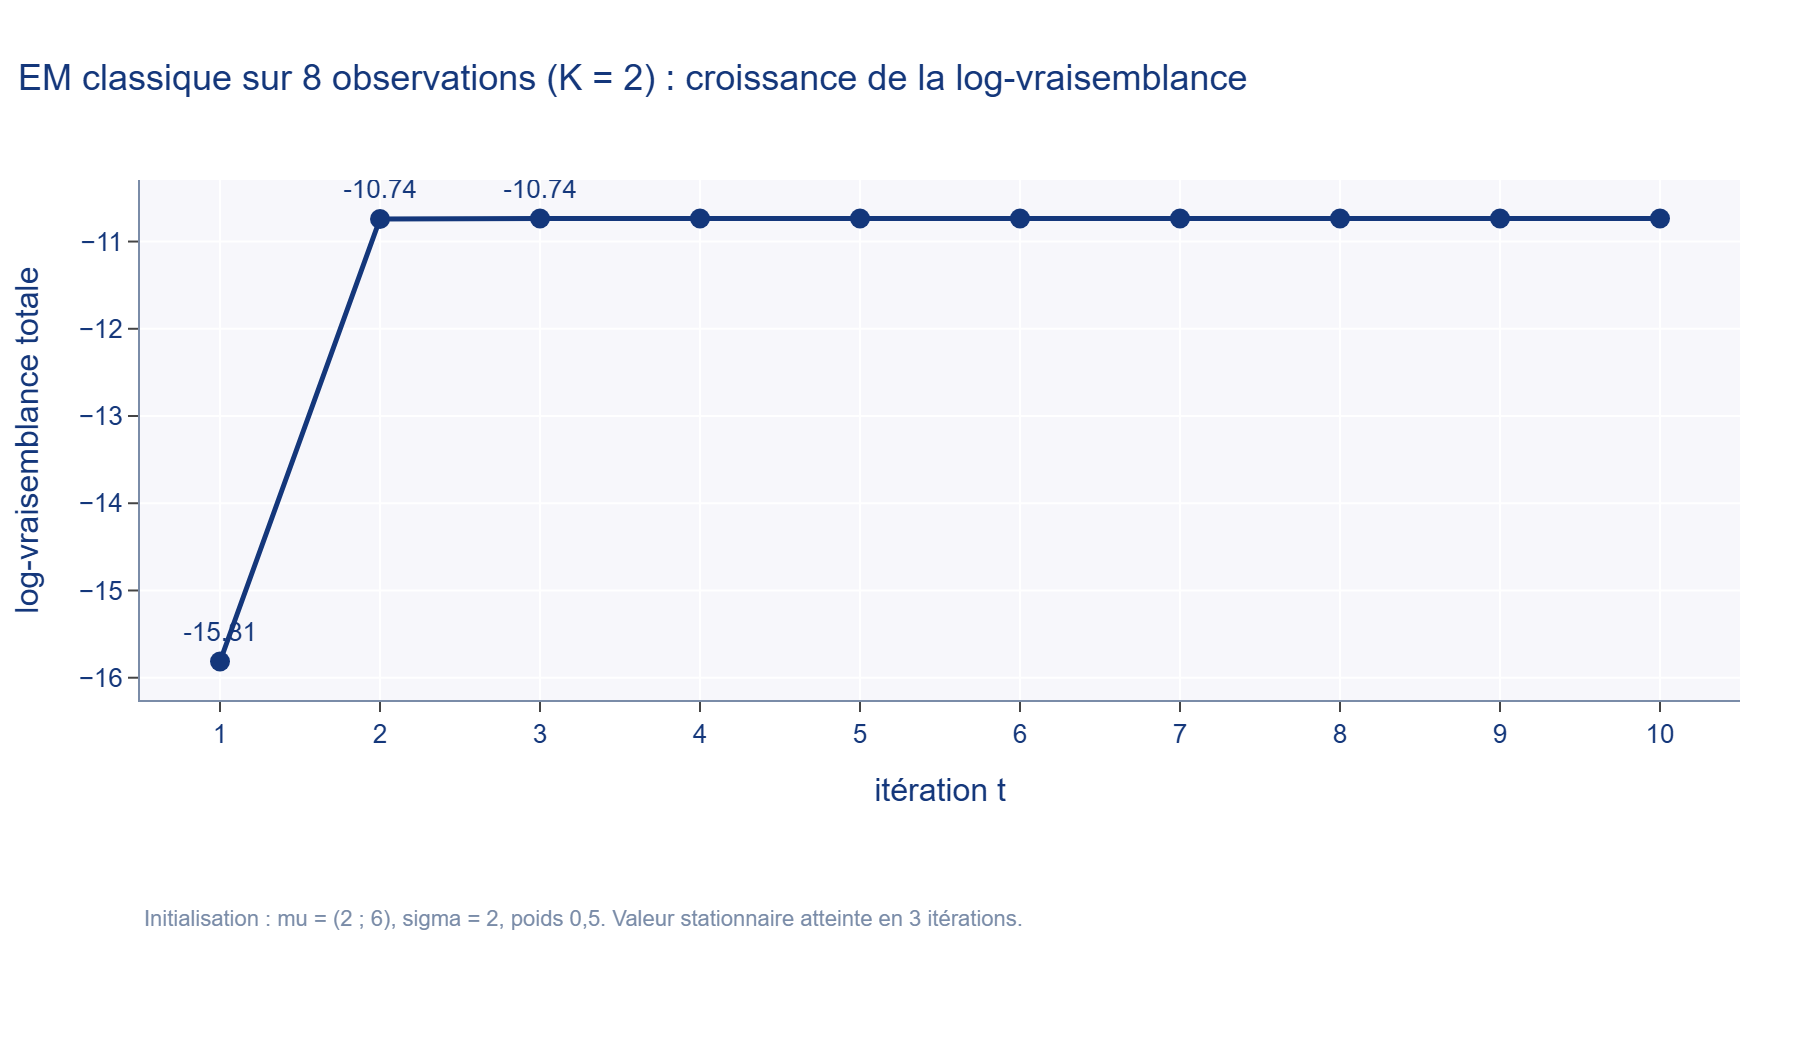
\includegraphics[width=0.85\textwidth]{figures/fig01.png}
\caption{Évolution de la log-vraisemblance au fil des itérations (exemple numérique de la section 1.6.4). La courbe est croissante puis stationnaire dès la troisième itération, ce qui illustre la garantie de monotonie établie à la section 1.6.2.f.}
\label{fig:1_1}
\end{figure}
\subsection{Variantes de l'EM classique}
\begin{table}[H]
\centering
\small
\setlength{\tabcolsep}{0.14cm}
\begin{tabular}{|p{3.54cm}|p{3.54cm}|p{3.54cm}|p{3.54cm}|}
\hline
\textbf{Variante} & \textbf{Modification} & \textbf{Avantage} & \textbf{Inconvénient} \\
\hline
EM standard & Aucune & Simple, convergence garantie & Lent sur grandes données \\
\hline
EM stochastique (SEM) & Étape E : tirage aléatoire & Évite certains optima locaux & Pas de monotonie \\
\hline
EM online & Mise à jour incrémentale & Scalable & Choix du taux d'apprentissage \\
\hline
EM généralisé (GEM) & Étape M approchée & Flexible & Convergence plus lente \\
\hline
EM accéléré (ECME) & Étape CM-E alternée & Convergence plus rapide & Complexité accrue \\
\hline
\end{tabular}
\caption{Principales variantes de l'algorithme EM classique}
\label{tab:1_3}
\end{table}
L'EM stochastique, proposé par Celeux et Diebolt (1985), modifie l'étape E en remplaçant le calcul des responsabilités par un tirage aléatoire : chaque observation est assignée à une seule composante selon la distribution définie par les responsabilités. Cette introduction de stochasticité permet d'éviter certains optima locaux, de calculer des estimations d'incertitude empiriques, et d'explorer plus largement l'espace des paramètres, au prix de la perte de la propriété de monotonie de la vraisemblance.

Pour les grandes bases de données, l'EM standard, dit « batch », traite l'ensemble des données à chaque itération, ce qui peut se révéler prohibitif. L'EM online, proposé par Sato et Ishii (2000) puis par Cappé et Moulines (2009), met à jour les paramètres après chaque observation ou mini-lot, réduisant drastiquement le coût par itération, et converge dans les mêmes conditions que l'EM standard sous des conditions de type Robbins-Monro sur le taux d'apprentissage.

L'EM généralisé remplace l'étape M exacte par une étape qui améliore, sans nécessairement maximiser, la fonction Q : on requiert seulement Q($\theta ^{t+1}$ | $\theta ^{t}$) $\geq $ Q($\theta ^{t}$ | $\theta ^{t}$), au lieu d'une maximisation exacte. La propriété de croissance monotone de la vraisemblance est préservée sous cette condition plus faible, ce qui rend le GEM utile lorsque l'étape M exacte est coûteuse ou n'admet pas de solution analytique.

Enfin, l'application originale ayant motivé l'article de Dempster et al. était précisément le traitement des données manquantes. Lorsque certaines composantes de $x_{i}$ sont manquantes, on peut traiter les valeurs manquantes comme des variables latentes supplémentaires, et l'algorithme EM impute naturellement ces valeurs en calculant leur espérance conditionnelle à l'étape E. Cette approche est asymptotiquement plus efficace que l'imputation simple et produit des estimateurs cohérents sous l'hypothèse MCAR ou MAR.

\subsection{Extension aux données séquentielles : l'algorithme de Baum-Welch}
Une application particulièrement importante de l'algorithme EM, mentionnée à plusieurs reprises dans ce mémoire (tableau 1.1, sections 1.6.1 et 3.1.3), concerne les modèles de Markov cachés (HMM), utilisés notamment en bio-informatique et en finance. Contrairement au GMM, où les observations sont supposées indépendantes conditionnellement à leur variable latente, un HMM suppose que la séquence des variables latentes ($z_{1}$, \ldots{}, z\_T) forme elle-même une chaîne de Markov : $z_{t}$ dépend de $z_{t-1}$ selon une matrice de transition A, et chaque observation $x_{t}$ dépend de l'état caché courant $z_{t}$ selon une matrice d'émission B. Cette structure séquentielle empêche le calcul direct des responsabilités comme à l'équation (1.15), puisque les variables latentes ne sont plus indépendantes entre elles : l'étape E doit être remplacée par l'algorithme forward-backward, qui exploite la structure de chaîne pour calculer efficacement, par programmation dynamique, les probabilités a posteriori nécessaires. L'algorithme résultant, connu sous le nom d'algorithme de Baum-Welch (Baum et al., 1970), est historiquement antérieur à la formalisation générale de Dempster, Laird et Rubin, mais en constitue, comme le notent ces derniers dans leur article de 1977, un cas particulier.

\textbf{Illustration numérique. }Considérons un HMM discret à deux états cachés (« Beau temps » = B, « Pluvieux » = P), avec une matrice de transition A = [[0,7 ; 0,3], [0,4 ; 0,6]] ($A_{ij}$ = P($z_{t+1}$=j | $z_{t}$=i)), et une matrice d'émission B qui associe à chaque état une probabilité d'observer « Parapluie » (Pa) ou « Pas de parapluie » (NPa) : B(B) = [0,1 ; 0,9] et B(P) = [0,8 ; 0,2]. Étant donné une courte séquence observée O = (NPa, Pa, Pa), l'étape E (forward-backward) calcule, pour chaque instant t et chaque état i, la probabilité a posteriori $\gamma _{t}$(i) = p($z_{t}$=i | O), de la même manière que $r_{ik}$ à l'équation (1.15) pour le GMM, mais en tenant compte de la dépendance séquentielle via les récursions forward $\alpha _{t}$(i) = [$\Sigma _{j}$ $\alpha _{t-1}$(j) $A_{ji}$] $B_{i}$($o_{t}$) et backward $\beta _{t}$(i) = $\Sigma _{j}$ $A_{ij}$ $B_{j}$($o_{t+1}$) $\beta _{t+1}$(j).

Une fois les quantités $\gamma _{t}$(i) calculées, l'étape M du Baum-Welch réestime les matrices A et B par des formules directement analogues à l'équation (1.16) du GMM, en remplaçant les responsabilités $r_{ik}$ par les quantités $\gamma _{t}$(i) et $\xi _{t}$(i,j) = p($z_{t}$=i, $z_{t+1}$=j | O) : Â$_{ij}$ = $\Sigma _{t}$ $\xi _{t}$(i,j) / $\Sigma _{t}$ $\gamma _{t}$(i), et $\hat{B}$$_{i}$(v) = $\Sigma $\_\{t : $o_{t}$=v\} $\gamma _{t}$(i) / $\Sigma _{t}$ $\gamma _{t}$(i). Cette correspondance formelle entre les mises à jour du Baum-Welch et celles du GMM illustre concrètement l'affirmation, faite à la section 1.6.1, selon laquelle l'EM constitue un cadre général unifiant des algorithmes historiquement développés de façon indépendante : le Baum-Welch n'est rien d'autre qu'un EM classique dans lequel l'étape E est rendue efficace, par programmation dynamique, pour tenir compte de la dépendance séquentielle entre variables latentes successives  une adaptation que l'on retrouve, sous une forme analogue, dans les extensions séquentielles de l'EM variationnel évoquées à la section 1.7.7.

\textbf{Calcul numérique complet de l'étape E. }Pour rendre entièrement concret le mécanisme décrit ci-dessus, calculons explicitement les quantités forward $\alpha _{t}$(i), backward $\beta _{t}$(i) et les probabilités a posteriori $\gamma _{t}$(i) pour la séquence observée O = (NPa, Pa, Pa), avec les matrices A et B et la distribution initiale $\pi _{0}$ = (0,6 ; 0,4) données ci-dessus. Le tableau 1.4 présente le détail de ce calcul.

\tableauGenere{t1_4}
La dernière colonne du tableau se lit comme suit : après observation de la séquence complète (NPa, Pa, Pa), la probabilité a posteriori que le temps ait été « Beau » (B) au premier instant est de 0,791 (malgré l'absence de parapluie ce jour-là, cohérent avec un temps beau), tandis qu'elle chute à 0,127 au deuxième instant et à 0,096 au troisième, la présence du parapluie aux instants 2 et 3 rendant l'état « Pluvieux » (P) très majoritairement probable a posteriori ($\gamma _{2}$(P) = 0,873 et $\gamma _{3}$(P) = 0,904). On notera que $\Sigma _{i}$ $\gamma _{t}$(i) = 1 à chaque instant t, exactement comme $\Sigma _{k}$ $r_{ik}$ = 1 pour les responsabilités du GMM à l'équation (1.15)  les quantités $\gamma _{t}$(i) jouant, pour le HMM, exactement le rôle que jouent les responsabilités $r_{ik}$ pour le GMM. La probabilité totale de la séquence observée, obtenue en sommant $\alpha _{t}$(i) sur i au dernier instant, vaut p(O | A, B, $\pi _{0}$) = $\alpha _{3}$(B) + $\alpha _{3}$(P) = 0,010 + 0,091 = 0,100.

\subsection{Avantages de l'EM classique}
\begin{itemize}
\item \textbf{Simplicité et transparence : }l'algorithme EM est conceptuellement clair et facile à comprendre. Les deux étapes E et M ont des interprétations directes, et les mises à jour sont souvent analytiques, ce qui facilite l'implémentation, le débogage et l'adaptation à de nouveaux modèles.
\item \textbf{Garantie de convergence monotone : }la log-vraisemblance ne peut que croître ou rester constante à chaque itération. Cette propriété offre une sécurité précieuse : l'algorithme ne peut pas « se dégrader » au fil des itérations, et la log-vraisemblance constitue un critère de convergence naturel.
\item \textbf{Efficacité computationnelle par itération : }chaque itération de l'EM a un coût fixe en O($NKD^{2}$), aisément vectorisable. Pour des problèmes de taille modérée, l'EM est extrêmement rapide et se parallélise bien.
\item \textbf{Applicabilité universelle : }l'EM s'applique à n'importe quel modèle probabiliste pour lequel p(Z | X, $\theta $) est calculable et $\mathbb{E}$[log p(X, Z | $\theta $)] est maximisable, ce qui couvre une immense variété de modèles en pratique.
\item \textbf{Gestion naturelle des données incomplètes : }par construction, l'EM intègre sur les valeurs manquantes, produisant des estimateurs asymptotiquement efficaces sans recourir à des heuristiques d'imputation.
\item \textbf{Convergence rapide loin de l'optimum : }bien que la convergence soit linéaire asymptotiquement, l'EM converge souvent très rapidement lors des premières itérations, permettant d'obtenir de bonnes solutions en peu d'itérations.
\end{itemize}
\par\noindent\emph{Renvois à la grille du tableau~\ref{tab:2_17} :} garantie de croissance $\to$ ligne « Monotonie du critère » (théorème, tests unitaires) ; efficacité par itération et convergence rapide loin de l'optimum $\to$ « Coût de calcul » ; simplicité, applicabilité universelle et données incomplètes $\to$ affirmations qualitatives ou théoriques sans ligne expérimentale (« non testé » dans ce mémoire).
\subsection{Inconvénients et limites de l'EM classique}
\begin{itemize}
\item \textbf{Convergence vers des optima locaux : }l'EM converge vers un point stationnaire de la vraisemblance, généralement un maximum local. Sur les problèmes multimodaux, comme les GMM à composantes proches, la solution trouvée peut être significativement sous-optimale par rapport au maximum global.
\item \textbf{Nécessité de spécifier K a priori : }le nombre de composantes K doit être fixé avant l'exécution de l'algorithme. Une mauvaise spécification de K conduit inévitablement à des résultats sous-optimaux : la sous-estimation entraîne des composantes trop larges fusionnant des groupes distincts, tandis que la surestimation entraîne des composantes redondantes ou dégénérées. C'est précisément cette limite que nous illustrerons expérimentalement au chapitre 2, à travers un cas où K est volontairement surestimé.
\item \textbf{Incertitude non native : }l'EM classique fournit une estimation ponctuelle $\hat{\theta}$ ; une incertitude s'obtient a posteriori (formule de Louis, 1982, bootstrap, EM supplémenté de Meng et Rubin, 1991, EM stochastique), au prix de calculs supplémentaires. Ces intervalles sont de confiance, non de crédibilité (section 1.6.3.c).
\item \textbf{Singularités et dégénérescences : }un problème bien connu du GMM est la possibilité de convergence vers des solutions singulières, une composante pouvant s'effondrer sur un seul point de données, sa variance tendant vers zéro, ce qui provoque une divergence de la log-vraisemblance vers l'infini. Des stratégies ad hoc, telles que la régularisation de la covariance, sont nécessaires pour éviter ce problème.
\item \textbf{Lenteur de convergence : }le taux de convergence linéaire peut rendre l'algorithme très lent dans les régions proches de l'optimum, en particulier lorsque les composantes se chevauchent fortement. Ce défaut n'est pas propre à l'EM classique : l'EM variationnel batch a le même ordre de coût par itération (section 2.2.1) ; la comparaison du nombre d'itérations exige un critère d'arrêt commun (sections 2.3.1 et 2.3.8).
\item \textbf{Scalabilité limitée : }la version batch standard nécessite de traiter toutes les données à chaque itération, ce qui devient prohibitif pour des bases de plusieurs millions d'observations, sans recourir aux variantes online ou mini-batch. La même limite vaut pour la version batch de l'EM variationnel ; les variantes online (EM online) et stochastique (SVI) existent pour les deux (sections 1.6.5 et 1.7.7).
\end{itemize}
\par\noindent\emph{Renvois à la grille du tableau~\ref{tab:2_17} :} optima locaux $\to$ « Initialisation » (expérience unique) ; $K$ à fixer $\to$ « Sélection de $K$ », « Sous-estimation de $K$ » ; incertitude non native $\to$ « Incertitude » ; singularités $\to$ « Singularités, petit $N$ » et « Convergence de l'EM pour le GMM » ; lenteur et scalabilité $\to$ « Coût de calcul ».
\section{L'algorithme EM variationnel}
\subsection{Motivation et cadre général}
Les limitations identifiées à la section 1.6.8 motivent naturellement le développement d'une approche plus riche. L'EM variationnel émerge à la confluence de deux courants : l'inférence bayésienne, qui traite les paramètres comme des variables aléatoires et vise à caractériser leur distribution a posteriori complète, et l'optimisation variationnelle, qui transforme le problème d'inférence  généralement intractable  en un problème d'optimisation sur un espace de distributions plus simples.

Le cadre variationnel trouve ses racines dans les travaux de Hinton et van Camp (1993) sur les réseaux de neurones bayésiens, de Peterson et Anderson (1987) sur les champs moyens pour les réseaux de Boltzmann, et a été synthétisé et généralisé par Jordan, Ghahramani, Jaakkola et Saul (1999) dans leur article fondateur sur les méthodes variationnelles pour les modèles graphiques. Depuis lors, l'inférence variationnelle est devenue l'une des méthodes d'inférence approchée les plus utilisées en apprentissage automatique probabiliste. Pour le mélange gaussien, le traitement variationnel à priors conjugués est généralement rattaché à Attias (2000) et il est exposé en détail par Bishop (2006, section 10.2), dont ce travail suit les équations. Corduneanu et Bishop (2001) en donnent une variante distincte : les poids de mélange $\pi$ n'y reçoivent pas de prior de Dirichlet, ils sont traités comme des paramètres ponctuels et estimés par maximisation de la borne inférieure (maximum de vraisemblance de type II), tandis que $(\mu_k, \Lambda_k)$ restent aléatoires (section 1.7.4). L'article d'Attias n'a pas été consulté dans le texte original ; il n'est cité que pour l'historique.

\subsection{Inférence variationnelle}
\subsubsection{a) Le problème d'inférence bayésienne}
Dans le cadre bayésien complet, on cherche à calculer la distribution a posteriori jointe sur les paramètres et les variables latentes, p($\theta $, Z | X) = p(X | Z, $\theta $) p(Z | $\theta $) p($\theta $) / p(X). Le dénominateur, p(X) = $\int \int $ p(X | Z, $\theta $) p(Z | $\theta $) p($\theta $) dZ $d\theta $, est la vraisemblance marginale, ou évidence. Son calcul nécessite une intégrale de haute dimension, généralement intractable analytiquement pour des modèles non triviaux. Sans ce dénominateur, on ne peut pas normaliser la distribution a posteriori. L'inférence variationnelle contourne ce problème en remplaçant le calcul exact de p($\theta $, Z | X) par l'optimisation d'une approximation.

\subsubsection{b) La famille variationnelle et le problème d'optimisation}
L'inférence variationnelle introduit une famille de distributions $\mathcal{Q}$ = \{q($\theta $, Z | $\lambda $), $\lambda $ $\in $ $\Lambda $\}, paramétrée par des paramètres variationnels $\lambda $. L'objectif est de trouver le membre de cette famille le plus proche de la vraie distribution a posteriori, au sens de la divergence de Kullback-Leibler :

\begin{equation}
\begin{adjustbox}{max width=0.92\linewidth}$\displaystyle q*(\theta {,} Z) = \operatorname*{argmin}_{q \in  \mathcal{Q}} KL[q(\theta {,} Z) \Vert  p(\theta {,} Z | X)]$\end{adjustbox}
\tag{1.20}
\label{eq:1_20}
\end{equation}
Cette divergence ne peut pas être calculée directement, car elle fait intervenir p(X) dans sa normalisation. On montre cependant que minimiser cette divergence est équivalent à maximiser l'ELBO, qui lui est calculable :

\begin{equation}
\begin{adjustbox}{max width=0.92\linewidth}$\displaystyle ELBO(q) = \mathbb{E}_{q}[\log  p(X{,} Z{,} \theta )] - \mathbb{E}_{q}[\log  q(\theta {,} Z)]$\end{adjustbox}
\tag{1.21}
\label{eq:1_21}
\end{equation}
Cette reformulation est la clé de l'inférence variationnelle : un problème d'inférence, à savoir le calcul d'une distribution, est transformé en un problème d'optimisation, à savoir la maximisation d'une fonctionnelle de q, qui peut être traité par des algorithmes d'optimisation standard.

\subsubsection{c) L'ELBO comme objectif d'apprentissage}
L'ELBO peut être décomposé de deux manières complémentaires, chacune offrant une interprétation différente. La première décomposition montre l'ELBO comme la différence entre la vraisemblance attendue et la complexité du modèle :

\begin{equation}
\begin{adjustbox}{max width=0.92\linewidth}$\displaystyle ELBO(q) = \mathbb{E}_{q}[\log  p(X | Z{,} \theta )] - KL[q(\theta {,} Z) \Vert  p(\theta {,} Z)]$\end{adjustbox}
\tag{1.22}
\label{eq:1_22}
\end{equation}
Le premier terme, la log-vraisemblance attendue sous q, mesure la qualité de l'ajustement aux données ; le second terme, la divergence KL entre la distribution variationnelle et le prior joint, pénalise les distributions q qui s'écartent trop du prior, réalisant ainsi une forme de régularisation bayésienne automatique. La maximisation de l'ELBO réalise donc un compromis naturel entre ajustement aux données et fidélité au prior.

La seconde décomposition, déjà introduite à la section 1.5.3, montre l'ELBO comme une borne inférieure de la log-évidence : log p(X) = ELBO(q) + KL[q($\theta $, Z) $\Vert $ p($\theta $, Z | X)] $\geq $ ELBO(q). Cette décomposition est fondamentale pour la sélection de modèle bayésien : un modèle dont l'ELBO est plus élevé à la convergence est préférable, car son évidence est plus grande, ce qui implique qu'il explique mieux les données tout en contrôlant la complexité.

\subsection{Formulation de l'EM variationnel}
\subsubsection{a) L'hypothèse du champ moyen}
L'hypothèse la plus courante pour définir la famille variationnelle $\mathcal{Q}$ est l'hypothèse du champ moyen, qui suppose une factorisation complète de la distribution variationnelle sur les différentes variables :

\begin{equation}
\begin{adjustbox}{max width=0.92\linewidth}$\displaystyle q(\theta {,} Z) = q(\theta ) \prod _{i} q(z_{i}) = q(\pi ) \prod _{k} q(\mu _{k}{,} \Lambda _{k}) \prod _{i} q(z_{i})$\end{adjustbox}
\tag{1.23}
\label{eq:1_23}
\end{equation}
Cette hypothèse ignore les corrélations a posteriori entre les paramètres $\theta $ et les variables latentes Z, ainsi qu'entre les variables latentes de différentes observations. Si cette indépendance est rarement exacte dans la vraie distribution a posteriori, elle simplifie considérablement le problème d'optimisation en le rendant décomposable en sous-problèmes indépendants, tout en restant une approximation raisonnable dans de nombreuses applications.

\subsubsection{b) Les mises à jour variationnelles optimales}
Sous l'hypothèse du champ moyen, la solution variationnelle optimale pour chaque facteur $q_{j}$($z_{j}$) est donnée par la formule du champ moyen variationnel :

\begin{equation}
\begin{adjustbox}{max width=0.92\linewidth}$\displaystyle \log  q*_{j}(z_{j}) = \mathbb{E}_{q(z \setminus z_{j})}[\log  p(X{,} Z{,} \theta )] + constante$\end{adjustbox}
\tag{1.24}
\label{eq:1_24}
\end{equation}
Cette mise à jour prend l'espérance de la log-distribution jointe par rapport à tous les autres facteurs, en maintenant $z_{j}$ fixe, la constante additive assurant la normalisation. Cette formule est générale et s'applique à n'importe quel facteur, qu'il s'agisse d'une variable latente ou d'un paramètre. Dans le cas des modèles conjugués, cette espérance peut être calculée analytiquement et conduit à une distribution de la même famille que le prior correspondant.

\subsubsection{c) Dérivation détaillée pour le mélange gaussien bayésien}
Cette section applique explicitement la formule générale du champ moyen variationnel, énoncée ci-dessus, au cas particulier du mélange gaussien bayésien, afin de montrer comment les formes de Dirichlet et de Normal-Wishart, utilisées dans l'algorithme de la section 1.7.3.d, se déduisent directement de cette formule générale plutôt que d'être postulées arbitrairement.

\textbf{Facteur q($\pi $). }En isolant, dans le logarithme de la distribution jointe complète log p(X, Z, $\pi $, $\mu $, $\Lambda $), les seuls termes qui dépendent de $\pi $, on obtient log p(Z | $\pi $) + log p($\pi $) = $\Sigma _{i}$ $\Sigma _{k}$ $z_{ik}$ log $\pi _{k}$ + $\Sigma _{k}$ ($\alpha _{0}$-1) log $\pi _{k}$ + constante, où $z_{ik}$ désigne l'indicatrice $z_{i}$ = k. En appliquant la formule du champ moyen, on prend l'espérance de cette expression par rapport à q(Z), ce qui revient à remplacer $z_{ik}$ par son espérance $r_{ik}$ = $\mathbb{E}$\_q[$z_{ik}$] :

\begin{equation}
\begin{adjustbox}{max width=0.92\linewidth}$\displaystyle \log  q*(\pi ) = \Sigma _{k} (\alpha _{0} - 1 + N_{k}) \log  \pi _{k} + \text{constante}{,}\ \text{où}\ N_{k} = \Sigma _{i} r_{ik}$\end{adjustbox}
\tag{1.25}
\label{eq:1_25}
\end{equation}
Cette expression est, à une constante de normalisation près, exactement le logarithme de la densité d'une distribution de Dirichlet de paramètres $\alpha _{k}$ = $\alpha _{0}$ + $N_{k}$. On retrouve ainsi directement, par simple application de la formule générale, la mise à jour $\alpha _{k}$ = $\alpha _{0}$ + $N_{k}$ utilisée à la section 1.7.3.d, sans qu'il soit nécessaire de la postuler : elle découle mécaniquement de la conjugaison entre le prior de Dirichlet et la vraisemblance catégorielle.

\textbf{Facteur q($\mu _{k}$, $\Lambda _{k}$). }De façon similaire, en isolant les termes qui dépendent de ($\mu _{k}$, $\Lambda _{k}$) dans log p(X, Z, $\pi $, $\mu $, $\Lambda $), on obtient une contribution de la vraisemblance gaussienne, $\Sigma _{i}$ $r_{ik}$ log $\mathcal{N}$($x_{i}$ | $\mu _{k}$, $\Lambda _{k}^{-1}$), à laquelle s'ajoute le logarithme du prior Normal-Wishart log p($\mu _{k}$, $\Lambda _{k}$). Cette somme, une fois réorganisée en complétant le carré sur $\mu _{k}$  une manipulation algébrique standard pour les formes quadratiques gaussiennes , se réécrit comme le logarithme d'une densité Normal-Wishart de paramètres mis à jour :

\begin{equation}
\begin{adjustbox}{max width=0.92\linewidth}$\displaystyle \beta _{k} = \beta _{0} + N_{k}{,}   m_{k} = (\beta _{0}m_{0} + N_{k}\bar{x}_{k})/\beta _{k}{,}   \nu _{k} = \nu _{0} + N_{k}{,}   W_{k}^{-1} = W_{0}^{-1} + N_{k}S_{k} + [\beta _{0}N_{k}/(\beta _{0}+N_{k})](\bar{x}_{k}-m_{0})(\bar{x}_{k}-m_{0})^{T}$\end{adjustbox}
\tag{1.26}
\label{eq:1_26}
\end{equation}
où $\bar{x}$$_{k}$ et $S_{k}$ désignent respectivement la moyenne et la covariance empiriques pondérées par les responsabilités, telles que définies à la section 1.7.3.d. Le terme $\beta _{k}$ s'interprète comme une « taille d'échantillon effective augmentée » (la taille d'échantillon effective $N_{k}$ à laquelle s'ajoute la pseudo-taille d'échantillon $\beta _{0}$ du prior), tandis que le dernier terme correctif dans la mise à jour de $W_{k}^{-1}$ traduit l'incertitude supplémentaire due à l'écart entre la moyenne empirique du cluster $\bar{x}$$_{k}$ et la moyenne a priori $m_{0}$ : plus cet écart est grand par rapport à la confiance relative accordée au prior (mesurée par le rapport $\beta _{0}N_{k}$/($\beta _{0}$+$N_{k}$)), plus la matrice de précision $W_{k}^{-1}$ voit sa valeur augmenter, ce qui élargit d'autant la distribution a posteriori sur $\mu _{k}$.

Cette dérivation confirme, de façon rigoureuse, que les formules de mise à jour utilisées à la section 1.7.3.d ne sont pas de simples analogues heuristiques de l'étape M classique : elles sont la conséquence mathématique directe et nécessaire de l'application de la formule générale du champ moyen variationnel au choix spécifique de priors conjugués effectué à la section 1.4.2. Ce même schéma de dérivation  isoler les termes pertinents dans la log-distribution jointe, prendre leur espérance sous les autres facteurs, puis reconnaître la forme conjuguée résultante  se généralise sans difficulté conceptuelle à tout modèle à variables latentes construit à partir de distributions conjuguées, ce qui explique la popularité de l'hypothèse du champ moyen dans la pratique de l'inférence variationnelle.

\subsubsection{d) L'algorithme EM variationnel}
L'algorithme EM variationnel alterne entre deux étapes, analogues aux étapes E et M de l'EM classique, mais opérant sur des distributions plutôt que sur des estimations ponctuelles. L'algorithme prend en entrée les observations X, un nombre maximal de composantes Kmax, les hyperparamètres du prior \{$\alpha _{0}$, $m_{0}$, $\beta _{0}$, $W_{0}$, $\nu _{0}$\}, ainsi qu'un critère d'arrêt $\varepsilon $.

\textbf{Initialisation. }Les paramètres variationnels sont initialisés : $\alpha _{k}$ = $\alpha _{0}$ + N/K, $N_{k}$ = N/K, $m_{k}$ = $m_{0}$ + perturbation aléatoire, $\beta _{k}$ = $\beta _{0}$ + $N_{k}$, $\nu _{k}$ = $\nu _{0}$ + $N_{k}$, $W_{k}$ = $W_{0}$.

\textbf{Étape E variationnelle. }Pour chaque observation i et chaque composante k, on calcule :

\begin{equation}
\begin{adjustbox}{max width=0.92\linewidth}$\displaystyle \log  \rho _{ik} = \mathbb{E}[\log  \pi _{k}] + \tfrac{1}{2} \mathbb{E}[\log |\Lambda _{k}|] - (D/2) \log (2\pi ) - \tfrac{1}{2} \mathbb{E}[(x_{i}-\mu _{k})^{T}\Lambda _{k}(x_{i}-\mu _{k})]$\end{adjustbox}
\tag{1.27}
\label{eq:1_27}
\end{equation}
puis on normalise pour obtenir les responsabilités : $r_{ik}$ = exp(log $\rho _{ik}$) / $\Sigma _{j}$ exp(log $\rho _{ij}$).

\textbf{Étape M variationnelle. }Pour chaque composante k, on calcule $N_{k}$ = $\Sigma _{i}$ $r_{ik}$, $\bar{x}$$_{k}$ = (1/$N_{k}$) $\Sigma _{i}$ $r_{ik}$ $x_{i}$, et $S_{k}$ = (1/$N_{k}$) $\Sigma _{i}$ $r_{ik}$ ($x_{i}$-$\bar{x}$$_{k}$)($x_{i}$-$\bar{x}$$_{k}$)$^{T}$, avant de mettre à jour les paramètres des lois de Dirichlet et Normal-Wishart :

\begin{equation}
\begin{adjustbox}{max width=0.92\linewidth}$\displaystyle \alpha _{k} = \alpha _{0} + N_{k}{,}  \beta _{k} = \beta _{0} + N_{k}{,}  m_{k} = (\beta _{0}m_{0} + N_{k}\bar{x}_{k})/\beta _{k}{,}  \nu _{k} = \nu _{0} + N_{k}$\end{adjustbox}
\tag{1.28}
\label{eq:1_28}
\end{equation}
ainsi que la mise à jour de la matrice d'échelle $W_{k}^{-1}$ = $W_{0}^{-1}$ + $N_{k}S_{k}$ + [$\beta _{0}N_{k}$/($\beta _{0}$+$N_{k}$)] ($\bar{x}$$_{k}$-$m_{0}$)($\bar{x}$$_{k}$-$m_{0}$)$^{T}$. L'ELBO est ensuite calculé, et les composantes telles que $\alpha _{k}$ $\approx $ $\alpha _{0}$ sont élaguées, selon le mécanisme détaillé à la section 1.7.4. Ces deux étapes sont répétées jusqu'à convergence de l'ELBO, l'algorithme retournant alors la distribution q*($\theta $) ainsi que le nombre effectif de composantes actives, K\_effectif.

\subsubsection{e) Calcul des espérances nécessaires}
L'étape E variationnelle requiert le calcul de plusieurs espérances par rapport aux distributions variationnelles courantes, espérances qui admettent des formes analytiques pour les distributions conjuguées utilisées. Pour la distribution de Dirichlet q($\pi $) = Dir($\alpha _{1}$, \ldots{}, $\alpha K$), l'espérance du logarithme du poids est donnée par :

\begin{equation}
\begin{adjustbox}{max width=0.92\linewidth}$\displaystyle \mathbb{E}[\log  \pi _{k}] = \psi (\alpha _{k}) - \psi (\Sigma _{j} \alpha _{j})$\end{adjustbox}
\tag{1.29}
\label{eq:1_29}
\end{equation}
où $\psi $ désigne la fonction digamma. Pour la distribution de Wishart q($\Lambda _{k}$) = $\mathcal{W}$($W_{k}$, $\nu _{k}$), on obtient $\mathbb{E}$[log|$\Lambda _{k}$|] = $\Sigma _{j=1}^{D}$ $\psi $[($\nu _{k}$+1-j)/2] + D log 2 + log|$W_{k}$|. Enfin, pour la distribution normale q($\mu _{k}$|$\Lambda _{k}$) = $\mathcal{N}$($m_{k}$, ($\beta _{k}\Lambda _{k}$)$^{-1}$), l'espérance de la forme quadratique vaut :

\begin{equation}
\begin{adjustbox}{max width=0.92\linewidth}$\displaystyle \mathbb{E}[(x-\mu _{k})^{T}\Lambda _{k}(x-\mu _{k})] = D/\beta _{k} + \nu _{k}(x-m_{k})^{T}W_{k}(x-m_{k})$\end{adjustbox}
\tag{1.30}
\label{eq:1_30}
\end{equation}
\subsection{Sélection automatique du nombre de composantes}
L'une des propriétés les plus remarquables et pratiquement importantes de l'EM variationnel est sa capacité à déterminer automatiquement le nombre effectif de composantes dans un mélange gaussien bayésien. Ce mécanisme, qui constitue l'un des apports majeurs de l'EM variationnel par rapport à l'EM classique, mérite une explication détaillée, car il sera au cœur de l'étude expérimentale présentée au chapitre 2.

La clé de ce mécanisme réside dans le prior de Dirichlet Dir($\alpha _{0}$, \ldots{}, $\alpha _{0}$) placé sur les poids de mélange. Lorsque $\alpha _{0}$ est petit  typiquement $\alpha _{0}$ = 1/Kmax ou $\alpha _{0}$ = 10$^{-3}$ , ce prior favorise fortement les solutions parcimonieuses, où la plupart des poids sont proches de zéro, c'est-à-dire les solutions n'utilisant qu'un petit nombre de composantes actives.

Lors de l'optimisation variationnelle, l'élagage ne provient pas de l'espérance $\mathbb{E}[\pi_k] = (\alpha_0 + N_k)/(K\alpha_0 + N)$ : celle-ci est tirée vers la valeur uniforme $1/K$ pour tout $\alpha_0$ (section 1.4.4) et ne s'annule jamais. Il provient de l'espérance du logarithme du poids, qui intervient dans l'étape E (équation 1.29) :
\begin{equation*}
\mathbb{E}[\log \pi_k] = \psi(\alpha_k) - \psi\Big(\sum_{j}\alpha_j\Big), \qquad \alpha_k = \alpha_0 + N_k .
\end{equation*}
Pour $\alpha_k < 1$, on a $\psi(\alpha_k) = \psi(\alpha_k + 1) - 1/\alpha_k \approx -1/\alpha_k$, qui tend vers $-\infty$ quand $\alpha_k \to 0$. Une composante qui capte peu d'observations a donc un $\alpha_k$ proche de $\alpha_0$, un $\mathbb{E}[\log \pi_k]$ très négatif et des responsabilités $r_{ik}$ qui s'effondrent : $N_k$ diminue, ce qui accentue encore l'effet (rétroaction positive). La figure~\ref{fig:elagage} illustre ce mécanisme. Il est difficilement réversible : une composante dont $\alpha_k$ est tombé près de $\alpha_0$ ne reçoit plus de responsabilité et ne peut plus être réactivée par les itérations suivantes.

\begin{figure}[H]
\centering
\begin{tikzpicture}[x=2.6cm,y=0.62cm,>=Stealth]
  \draw[->] (0,0) -- (4.3,0) node[right] {$\alpha_k$};
  \draw[->] (0,-9) -- (0,2.2) node[above] {$\psi(\alpha_k)$};
  \foreach \x in {1,2,3,4} {\draw (\x,0.1) -- (\x,-0.1) node[below=3pt,font=\footnotesize] {\x};}
  \foreach \y in {-8,-6,-4,-2,0,2} {\draw (0.03,\y) -- (-0.03,\y) node[left,font=\footnotesize] {\y};}
  \draw[navy,very thick,domain=0.125:4,samples=90,smooth]
    plot (\x,{ln(\x+2)-1/(2*(\x+2))-1/(12*(\x+2)^2)-1/\x-1/(\x+1)});
  \draw[bleu,dashed] (1,-9) -- (1,2);
  \node[bleu,font=\footnotesize,anchor=west] at (1.03,1.6) {$\alpha_k=1$};
  \node[font=\footnotesize,anchor=west,text width=3.6cm] at (0.26,-7.3) {composante vide : $\alpha_k\approx\alpha_0$ petit, $\mathbb{E}[\log\pi_k]\ll 0$};
  \node[font=\footnotesize,anchor=east,text width=3.2cm,align=right] at (4.2,-3.3) {composante soutenue par les données : $\alpha_k=\alpha_0+N_k$ grand};
\end{tikzpicture}
\caption{Mécanisme d'élagage : $\psi(\alpha_k)\approx -1/\alpha_k$ tend vers $-\infty$ quand $\alpha_k\to 0$. Dans l'étape E, $\mathbb{E}[\log\pi_k]=\psi(\alpha_k)-\psi(\sum_j\alpha_j)$ pénalise une composante dont $\alpha_k$ reste proche de $\alpha_0$. Courbe tracée par l'approximation asymptotique de la fonction digamma décalée de 2.}
\label{fig:elagage}
\end{figure}


Le seuil en deçà duquel l'élagage opère n'est pas $\alpha_0 = 1$. Pour un mélange sur-paramétré, la théorie de Rousseau et Mengersen (2011) établit que la loi a posteriori exacte vide les composantes superflues lorsque $\alpha_0 < d/2$, où $d$ est le nombre de paramètres libres d'une composante ($d = 5$ pour une covariance pleine en dimension 2, soit un seuil de 2,5 ; $d = 4$ pour une covariance diagonale, seuil de 2 ; $d = 3$ pour une covariance sphérique, seuil de 1,5). Ce résultat concerne le posterior exact, non l'approximation de champ moyen. Son transfert à l'EM variationnel est donc une \emph{hypothèse à tester}, et non un fait acquis : l'expérience S8 (section 2.3.14) mesure le nombre de composantes actives sur une grille de $\alpha_0$ de 1 à 10 autour de ces seuils.

Ce mécanisme d'élagage automatique constitue une forme de rasoir d'Occam bayésien : le modèle utilise spontanément le nombre minimal de composantes nécessaires pour expliquer les données, sans sur-ajustement. En initialisant avec un Kmax suffisamment grand  par exemple Kmax = 20 pour un problème où l'on attend entre 3 et 5 groupes , l'algorithme converge naturellement vers une solution utilisant uniquement le nombre approprié de composantes actives, sans qu'il soit nécessaire d'exécuter l'algorithme séparément pour chaque valeur candidate de K, comme l'exigerait l'EM classique.

Ce rasoir d'Occam a un coût que le texte précédent ne doit pas masquer : le résultat dépend de $K_{\max}$ (il ne peut pas retrouver plus de composantes que $K_{\max}$), des hyperparamètres $(\alpha_0, \beta_0, \nu_0, W_0)$ qui déplacent la sensibilité de l'initialisation vers les priors, et du seuil d'activité choisi pour décréter qu'une composante est éteinte (le seuil $N_k \geq 1$ est une convention, dont la sensibilité est mesurée par l'expérience S10).

\textbf{Deux mécanismes d'élagage à ne pas confondre. }Le mécanisme décrit ci-dessus, par $\mathbb{E}[\log \pi_k]$, est celui du modèle entièrement bayésien de Bishop (2006, section 10.2), où $\pi$ suit un Dirichlet ; c'est celui que ce travail implémente. Corduneanu et Bishop (2001) obtiennent l'élagage autrement : $\pi$ est un paramètre ponctuel, réestimé par $\pi_k = N^{-1}\sum_n r_{nk}$ (Bishop, 2006, éq. 10.83), et les composantes qui contribuent peu à expliquer les données voient leur poids conduit à zéro au cours de l'optimisation, par un effet de détermination automatique de la pertinence. Dans la typologie de la section 2.1.2, cette variante est hybride : $\pi$ relève du niveau 2 (point estimé sur une borne marginale), $(\mu_k, \Lambda_k)$ du niveau 3. Les deux mécanismes partent d'un $K$ initial élevé et suppriment les composantes superflues en une seule exécution, mais ils n'ont ni les mêmes hyperparamètres (pas d'$\alpha_0$ chez Corduneanu et Bishop) ni la même lecture de l'incertitude sur les poids. Bishop (2006, section 10.2.4) signale en outre que, pour comparer des valeurs de $K$ par la borne, il faut tenir compte des $K!$ modes équivalents du posterior, par exemple en ajoutant $\ln K!$ à la borne.

\subsection{Exemple numérique illustratif}
Afin de rendre plus concret le mécanisme d'élagage décrit ci-dessus, reprenons l'exemple numérique de la section 1.6.4 : les huit observations scalaires X = \{0,5 ; 1,0 ; 1,2 ; 1,8 ; 7,1 ; 7,5 ; 8,0 ; 8,3\}, qui forment visiblement deux groupes bien séparés. Appliquons cette fois l'EM variationnel avec Kmax = 3 composantes  soit une de plus que le nombre réel de groupes , un prior de Dirichlet de concentration $\alpha _{0}$ = 1/3, et des priors Normal-Wishart non informatifs ($\beta _{0}$ = 10$^{-3}$, $\nu _{0}$ = 1, $W_{0}$ = 1).

L'algorithme converge en 5 à 15 itérations selon l'initialisation (critère $|\Delta \mathrm{ELBO}| < 10^{-6}$), vers la même solution dans les dix essais réalisés (graines 0 à 4, initialisation par les hyperparamètres ou par k-means). Le tableau 1.5 présente les paramètres finaux obtenus pour chacune des trois composantes.

\tableauGenere{t1_5}
Ce résultat illustre de façon particulièrement nette le mécanisme théorique décrit ci-dessus. Les deux premières composantes se partagent presque également la masse de probabilité (poids 0,482 chacune), avec des moyennes de 7,724 et 1,126 qui coïncident, à $10^{-3}$ près, avec les moyennes empiriques des deux groupes et avec la solution de l'EM classique de la section 1.6.4 (7,725 et 1,125). La troisième composante, en revanche, voit son paramètre $\alpha _{k}$ rester exactement égal à sa valeur initiale $\alpha _{0}$ = 1/3 = 0,333, signe que $N_{k}$ = $\alpha _{k}$ - $\alpha _{0}$ = 0 : aucune observation, même partiellement, ne lui a été attribuée au cours de la convergence. Cette composante est donc entièrement inactive, et le modèle retient effectivement K\_effectif = 2 composantes actives, exactement le nombre réel de groupes  un résultat que l'EM classique, avec K fixé à l'avance, ne peut pas produire de lui-même : il faudrait, pour l'EM classique, comparer explicitement les solutions à K = 2 et K = 3 au moyen d'un critère externe tel que le BIC, alors que l'EM variationnel effectue cette sélection de façon endogène, en une seule exécution.

\subsection{Calcul de l'ELBO et critère de convergence}
Pour le mélange gaussien bayésien sous l'hypothèse du champ moyen, l'ELBO peut être calculé analytiquement à chaque itération. Il se décompose sous la forme :

\begin{equation}
\begin{adjustbox}{max width=0.92\linewidth}$\displaystyle ELBO = \mathbb{E}_{q}[\log  p(X|Z{,}\theta )] + \mathbb{E}_{q}[\log  p(Z|\pi )] + \mathbb{E}_{q}[\log  p(\pi )] + \Sigma _{k} \mathbb{E}_{q}[\log  p(\mu _{k}{,}\Lambda _{k})] - \mathbb{E}_{q}[\log  q(Z)] - \mathbb{E}_{q}[\log  q(\pi )] - \Sigma _{k} \mathbb{E}_{q}[\log  q(\mu _{k}{,}\Lambda _{k})]$\end{adjustbox}
\tag{1.31}
\label{eq:1_31}
\end{equation}
Chacun de ces termes peut être calculé analytiquement grâce aux formes conjuguées des distributions considérées ; leur expression complète est donnée par Bishop (2006, éq. 10.71 à 10.77) et implémentée à l'annexe B. L'ELBO constitue le critère de convergence naturel de l'EM variationnel : on arrête l'algorithme lorsque |ELBO(t) - ELBO(t-1)| < $\varepsilon $. Contrairement à l'EM classique, où la log-vraisemblance peut diverger vers l'infini en présence de singularités, l'ELBO de l'EM variationnel reste toujours borné, grâce à la régularisation bayésienne induite par les priors.

\subsection{Variantes avancées de l'EM variationnel}
\textbf{Inférence variationnelle naturelle. }L'inférence variationnelle standard utilise le gradient ordinaire de l'ELBO pour optimiser les paramètres variationnels. Une variante plus efficace utilise le gradient naturel, qui prend en compte la géométrie de l'espace des distributions à travers la métrique de Fisher. Les mises à jour par gradient naturel sont invariantes aux reparamétrisations et convergent généralement beaucoup plus rapidement que les mises à jour utilisant le gradient ordinaire.

Les trois méthodes suivantes répondent chacune à une limite précise de l'EM variationnel batch à champ moyen : le coût d'un passage complet sur les données (SVI), le calcul analytique des espérances (VAE), la rigidité de la famille factorisée (flux normalisants). Seule la première est implémentée dans ce travail ; les deux autres sont présentées pour situer le VB conjugué dans l'état de l'art, et aucune conclusion expérimentale ne s'appuie sur elles.

\textbf{Inférence variationnelle stochastique (SVI). }Hoffman, Blei, Wang et Paisley (2013) considèrent les modèles à variables cachées \emph{globales} $\beta$, partagées par toutes les observations, et \emph{locales} $z_n$, propres à chaque observation et conditionnellement indépendantes des autres sachant $\beta$ (section 2.1 de l'article). Le GMM bayésien entre dans ce cadre : $(\pi, \mu_k, \Lambda_k)$ sont globales, $z_n$ est locale. Lorsque les lois conditionnelles complètes sont dans la famille exponentielle, le gradient naturel de l'ELBO par rapport au paramètre naturel global $\lambda$ (gradient prémultiplié par l'inverse de l'information de Fisher de $q(\beta)$) a une forme simple : il vaut la différence entre le paramètre de la loi conditionnelle optimale et $\lambda$. La SVI tire un mini-lot, calcule les paramètres locaux optimaux, forme une estimation bruitée $\hat\lambda$ de ce paramètre optimal en multipliant les statistiques du lot par $N/B$, puis met à jour $\lambda \leftarrow (1 - \rho_t)\lambda + \rho_t \hat\lambda$. Le pas $\rho_t = (t + \tau)^{-\kappa}$, avec un taux d'oubli $\kappa \in (0{,}5 ; 1]$ et un délai $\tau \geq 0$, satisfait les conditions de Robbins et Monro ($\sum_t \rho_t = \infty$, $\sum_t \rho_t^2 < \infty$). Les auteurs l'appliquent à la LDA et au processus de Dirichlet hiérarchique sur 350\,000 articles de \emph{Nature}, 1,8 million d'articles du \emph{New York Times} et 3,8 millions d'articles de Wikipédia. La fonction \texttt{svi\_gmm} applique exactement cette mise à jour aux paramètres naturels Normal-Wishart et Dirichlet du GMM (annexe A) ; elle sert de vérification et non de bras de comparaison. La SVI est l'analogue, pour le VB, de l'EM online (section 1.6.5) ; elle hérite de la même difficulté de réglage du pas.

\textbf{Auto-encodeurs variationnels et inférence amortie (AEVB). }Kingma et Welling (2014) traitent les modèles dont les variables latentes \emph{continues} ont un posterior intractable et dont les espérances de l'ELBO n'ont pas de forme close. Ils réécrivent un tirage de $q_\phi(z \mid x)$ comme une transformation différentiable d'un bruit, $z = g_\phi(\varepsilon, x)$ avec $\varepsilon \sim p(\varepsilon)$ (astuce de reparamétrisation), ce qui donne un estimateur sans biais et différentiable de la borne (estimateur SGVB), optimisable par gradient stochastique. Lorsque chaque observation a ses propres variables latentes, un réseau de reconnaissance (encodeur) $q_\phi(z \mid x)$ fournit directement les paramètres variationnels de chaque observation : l'inférence est \emph{amortie}, sans optimisation propre à chaque point. Deux limites bornent son intérêt pour ce travail. La reparamétrisation suppose $z$ continu, alors que l'indicateur d'appartenance du GMM est discret ; et l'optimisation par gradient stochastique ne conserve ni les mises à jour en forme close ni la croissance monotone de l'ELBO du VB conjugué.

\textbf{Flux normalisants. }Rezende et Mohamed (2015) enrichissent la famille variationnelle en transformant une loi initiale simple $q_0$ par une suite de bijections $f_1, \ldots, f_K$ : si $z_K = f_K \circ \cdots \circ f_1(z_0)$, alors $\ln q_K(z_K) = \ln q_0(z_0) - \sum_{k=1}^K \ln \lvert \det \partial f_k / \partial z_{k-1} \rvert$. Pour que ce terme reste calculable, ils proposent des flux \emph{planaires}, $f(z) = z + u\,h(w^\top z + b)$, dont le déterminant jacobien vaut $\lvert 1 + u^\top h'(w^\top z + b)\,w \rvert$ et se calcule en $O(D)$ par le lemme du déterminant matriciel, et des flux \emph{radiaux}, qui contractent ou dilatent la densité autour d'un point de référence. Ils soutiennent que, dans le régime asymptotique d'un flux de longueur croissante, la famille obtenue peut approcher le vrai posterior, ce que le champ moyen ne permet pas. C'est le remède au second effet de la section 1.5.4 (sous-estimation de la variance par factorisation) ; il n'est pas évalué ici, et son coût est d'abandonner, là encore, les mises à jour conjuguées.

\subsection{Avantages de l'EM variationnel}
\begin{itemize}
\item \textbf{Quantification complète de l'incertitude : }l'EM variationnel fournit une distribution q*($\theta $) sur les paramètres, permettant de calculer des intervalles de crédibilité, des quantiles, et d'intégrer l'incertitude paramétrique dans les prédictions, propriété fondamentale dans les applications où la décision doit tenir compte de l'incertitude. Cette distribution est une approximation (section 1.5.4) : sa fiabilité est mesurée par la couverture empirique de l'hypothèse H6.
\item \textbf{Sélection automatique du nombre de composantes : }le mécanisme d'élagage variationnel détermine automatiquement le nombre effectif de composantes, éliminant la nécessité d'une sélection externe de K et permettant une inférence en une seule exécution plutôt qu'une série d'exécutions pour différentes valeurs de K, au prix du choix de $K_{\max}$ et des hyperparamètres. Le gain en temps n'est pas acquis : il doit être mesuré en temps total jusqu'au modèle final (hypothèse H4).
\item \textbf{Régularisation bayésienne et robustesse : }l'intégration des distributions a priori protège naturellement contre le surapprentissage et les singularités, la divergence de Kullback-Leibler vers le prior dans l'ELBO agissant comme une régularisation qui empêche les composantes de s'effondrer sur des observations individuelles.
\item \textbf{ELBO comme critère de convergence : }l'ELBO borne inférieurement la log-évidence et fournit un critère de convergence croissant. Pour comparer des modèles, l'ELBO peut servir à comparer des valeurs de $K$ \emph{au sein du même algorithme variationnel}, avec les réserves de Corduneanu et Bishop (2001) : l'écart entre l'ELBO et la log-évidence (une divergence KL) varie d'un modèle à l'autre, ce qui biaise la comparaison. L'ELBO n'est pas comparable à un BIC ou à une log-vraisemblance d'EM (sections 2.2.3 et 2.3.3) : cette position est la seule retenue dans ce mémoire.
\item \textbf{Cadre extensible aux modèles complexes : }le cadre variationnel s'étend naturellement aux modèles hiérarchiques complexes, aux modèles génératifs profonds tels que les VAE, ainsi qu'aux modèles comportant plusieurs niveaux de variables latentes, là où l'EM classique devient difficilement applicable.
\item \textbf{Convergence monotone de l'ELBO : }comme l'EM classique, l'EM variationnel garantit que l'ELBO ne décroît jamais entre deux itérations, propriété qui assure une grande stabilité numérique et facilite le diagnostic de la convergence.
\end{itemize}
\par\noindent\emph{Renvois à la grille du tableau~\ref{tab:2_17} :} incertitude $\to$ « Incertitude » et « Gestion du risque » ; sélection automatique de $K$ $\to$ « Sélection de $K$ », « Seuil d'élagage » ; régularisation et robustesse $\to$ « Singularités, petit $N$ », « Valeurs aberrantes » ; ELBO et monotonie $\to$ « Monotonie du critère » ; extensibilité (VAE, flux normalisants) $\to$ « Vitesse de VAE, flux normalisants, gradient naturel » (non testé).
\subsection{Inconvénients et limites de l'EM variationnel}
\begin{itemize}
\item \textbf{Biais d'approximation systématique : }l'hypothèse du champ moyen introduit un biais systématique dans l'approximation. La distribution variationnelle optimale q* tend généralement à sous-estimer la variance de la véritable distribution a posteriori, phénomène de zero-forcing lié à la divergence KL. Lorsque la distribution a posteriori est fortement multimodale ou présente de fortes corrélations, cette approximation peut devenir relativement grossière.
\item \textbf{Complexité d'implémentation : }la dérivation des mises à jour variationnelles pour un nouveau modèle nécessite une bonne maîtrise du calcul variationnel bayésien ainsi que de la famille exponentielle. L'implémentation correcte du calcul de l'ELBO pour le suivi de la convergence est sensiblement plus complexe que celle de l'EM classique.
\item \textbf{Sensibilité aux distributions a priori : }le choix des hyperparamètres des distributions a priori ($\alpha _{0}$, $m_{0}$, $\beta _{0}$, $W_{0}$, $\nu _{0}$) peut influencer de manière significative les résultats, particulièrement lorsque le nombre de données disponibles est limité, ce qui nécessite une expertise ou une procédure de calibration empirique.
\item \textbf{Convergence vers des optima locaux de l'ELBO : }la maximisation de l'ELBO reste susceptible de converger vers des optima locaux. Bien que la régularisation bayésienne rende généralement la surface d'optimisation plus lisse que dans l'EM classique, ce problème n'est pas totalement éliminé, et plusieurs initialisations demeurent recommandées.
\item \textbf{Coût computationnel par itération plus élevé : }le calcul des différentes espérances variationnelles, impliquant notamment les fonctions digamma, les déterminants et les opérations matricielles, entraîne un surcoût computationnel à chaque itération par rapport à l'EM classique. Pour des problèmes simples, ce coût supplémentaire peut ne pas être compensé par les bénéfices apportés.
\item \textbf{Applicabilité restreinte aux modèles conjugués : }les mises à jour analytiques fermées de l'EM variationnel ne sont disponibles que pour les modèles utilisant des distributions conjuguées. Pour les modèles non conjugués, il est nécessaire de recourir à des méthodes d'approximation supplémentaires, telles que les gradients stochastiques, les approximations de Laplace ou les méthodes de quadrature, ce qui augmente davantage la complexité de l'algorithme.
\item \textbf{Irréversibilité de l'élagage : }une composante dont le poids s'est effondré ne reçoit plus de responsabilité et ne peut plus revenir (section 1.7.4). Une mauvaise trajectoire initiale peut donc éliminer définitivement une composante utile. Cet effet n'a pas été testé directement dans ce mémoire (« non testé » dans la grille de synthèse).
\item \textbf{Dépendance à $K_{\max}$ : }l'élagage ne peut retrouver que $K \leq K_{\max}$ composantes ; la sélection de $K$ est déplacée vers le choix de $K_{\max}$ et des hyperparamètres.
\item \textbf{Garanties fréquentistes partielles : }aucun résultat connu de ce travail ne garantit que l'élagage du champ moyen sélectionne le bon $K$ ; les résultats sur les mélanges sur-paramétrés (Rousseau et Mengersen, 2011) portent sur le posterior exact. Pour les paramètres, à $K$ fixé, les garanties existent mais sont partielles. Wang et Titterington (2006), cités par la revue de Blei et al. (2017, section 5.2), montrent pour le mélange gaussien à priors conjugués et champ moyen que l'algorithme CAVI converge vers un optimum local, que la moyenne variationnelle est consistante et qu'elle s'écarte du maximum de vraisemblance d'un terme en $O(1/n)$ ; Wang et Titterington (2005) montrent que la covariance variationnelle asymptotique est « trop petite », inférieure à l'inverse de l'information de Fisher d'une matrice définie positive. Ces deux articles n'ont pas été consultés directement. Plus généralement, Zhang et Gao (2020) bornent le taux de contraction du posterior variationnel par la somme de deux termes : le taux $\varepsilon_n^2$ du posterior exact, établi par les conditions classiques de « masse a priori et tests », et l'erreur d'approximation $\frac{1}{n}\inf_{Q \in \mathcal{S}} P_0\,D(Q \,\Vert\, \Pi(\cdot \mid X))$ propre à la famille $\mathcal{S}$. Pour un prior produit et la famille du champ moyen, une condition de masse a priori renforcée suffit à rendre le second terme négligeable devant le premier. Ces résultats portent sur une famille variationnelle définie sur les \emph{paramètres} ; leur application aux mélanges (section 4.3 de l'article) concerne l'estimation de densité en distance de Hellinger, avec une famille qui ne factorise pas les poids entre eux et sans facteur $q(Z)$ sur les affectations. Ils ne s'appliquent donc pas tels quels au VB de ce travail, qui factorise $q(Z)\,q(\pi, \mu, \Lambda)$. Le résultat de type Bernstein-von Mises de Wang et Blei (2019) pour les modèles paramétriques, cité par Zhang et Gao, n'a pas été consulté. La sous-couverture mesurée par l'hypothèse H6 est cohérente avec le résultat de Wang et Titterington (2005), sans en constituer une vérification.
\item \textbf{Double usage des données avec des priors empiriques : }fixer $m_0$ et $W_0^{-1}$ à partir des données (Bayes empirique) utilise l'échantillon deux fois ; l'ELBO et les intervalles de crédibilité n'ont plus leur lecture bayésienne stricte. Un jeu de priors fixés avant les données doit être comparé (expérience S9).
\end{itemize}
\par\noindent\emph{Renvois à la grille du tableau~\ref{tab:2_17} :} biais d'approximation $\to$ « Biais d'approximation » et « Incertitude » (couverture) ; sensibilité aux priors $\to$ « Sensibilité aux priors », « Seuil d'élagage » ; optima locaux de l'ELBO $\to$ « Optima locaux de l'ELBO » (non testé) ; coût par itération $\to$ « Coût de calcul » ; irréversibilité de l'élagage, dépendance à $K_{\max}$, consistance, double usage des données $\to$ lignes homonymes (« non testé » ou « expérience unique ») ; complexité d'implémentation et conjugaison $\to$ affirmations qualitatives sans ligne expérimentale.
\section{Conclusion du chapitre 1}
Ce premier chapitre a permis de poser l'ensemble des fondements théoriques nécessaires à la compréhension des deux algorithmes centraux de ce mémoire. Nous avons vu que les modèles à variables latentes, et en particulier le modèle de mélange gaussien, fournissent un cadre unificateur dans lequel s'inscrivent naturellement l'EM classique et l'EM variationnel. L'inégalité de Jensen et la borne ELBO constituent le socle mathématique commun aux deux algorithmes, tandis que le cadre bayésien et la divergence de Kullback-Leibler permettent de comprendre précisément ce qui distingue l'approche variationnelle de l'approche classique.

Ce parcours théorique n'a pas été conduit de façon purement abstraite : chaque notion introduite  la borne ELBO, la conjugaison Dirichlet--Catégorielle, le mécanisme d'élagage bayésien, la correspondance avec l'algorithme de Baum-Welch  a été illustrée par un exemple numérique (calculé à la main pour la densité du GMM et la conjugaison Dirichlet--Catégorielle ; produit par le code et vérifié pour les tableaux 1.2, 1.4 et 1.5), du plus simple (l'évaluation de la densité d'un GMM à deux composantes, section 1.3.5) au plus élaboré (le calcul complet des quantités forward, backward et a posteriori d'un modèle de Markov caché, section 1.6.6). Cette démarche, délibérément choisie, répond à la conviction que la compréhension approfondie d'un algorithme d'inférence statistique passe nécessairement par la capacité à en dérouler, à la main ou par le calcul, chacune des étapes sur un exemple de taille réduite, avant d'en confier l'exécution à une bibliothèque logicielle  démarche qui trouve son prolongement naturel dans les implémentations from scratch présentées au chapitre 3.

L'étude détaillée de l'EM classique a mis en évidence sa simplicité, son efficacité computationnelle et la garantie de convergence monotone qui le caractérisent, mais également ses limites majeures : nécessité de fixer K a priori, absence de quantification de l'incertitude, et sensibilité aux singularités. Les résultats non asymptotiques récents (section 1.6.3.d) précisent ces limites : en sur-spécification équilibrée, l'EM converge lentement vers une estimation de précision $(d/n)^{1/4}$ seulement, et en sous-spécification il vise la projection de Kullback-Leibler de la vraie loi, non un paramètre vrai. L'étude de l'EM variationnel a montré que le cadre bayésien ne lève pas ces limites mais les déplace : la sélection de $K$ passe du critère externe aux hyperparamètres et à $K_{\max}$, l'incertitude devient native mais approchée et vraisemblablement trop étroite (section 1.7.9), le tout au prix d'une complexité d'implémentation et d'un coût par itération plus élevés. Les extensions modernes (SVI, inférence amortie, flux normalisants, section 1.7.7) répondent chacune à l'une de ces limites, sans être évaluées ici. La dérivation détaillée du champ moyen variationnel pour le cas particulier du GMM bayésien (section 1.7.3.c) a par ailleurs montré que les formules de mise à jour de l'EM variationnel, loin d'être postulées par analogie avec l'EM classique, se déduisent rigoureusement de l'application d'un principe unique  la formule générale du champ moyen  à un choix spécifique de distributions conjuguées, ce qui confère à l'ensemble de l'édifice théorique une cohérence interne que l'on ne perçoit pas toujours dans les présentations plus informelles de la littérature d'introduction.

Le chapitre suivant s'attache à confronter directement ces deux algorithmes, sur les plans théorique, algorithmique et expérimental, à travers une étude de cas fondée sur un mélange de gaussiennes dont le nombre de composantes est volontairement surestimé  étude qui permettra de vérifier empiriquement, et non plus seulement théoriquement, chacune des propriétés établies dans ce premier chapitre.


%% ==== PARTIE 2 ====
\part{MÉTHODOLOGIE ET CADRE DE CONFRONTATION}

%% ==== CHAPITRE : COMPARAISON ENTRE L'EM CLASSIQUE ET L'EM VARIATIONNEL ====
\chapter{COMPARAISON ENTRE L'EM CLASSIQUE ET L'EM VARIATIONNEL}
Après avoir posé, au chapitre précédent, les fondements théoriques communs aux deux algorithmes et détaillé leur formulation mathématique respective, ce deuxième chapitre propose une confrontation directe et systématique entre l'EM classique et l'EM variationnel. Cette confrontation est menée en trois temps : une comparaison théorique, qui synthétise les différences conceptuelles entre les deux approches ; une comparaison algorithmique, qui examine leurs différences de complexité, de coût computationnel et de comportement numérique ; et enfin une étude expérimentale, fondée sur un mélange de gaussiennes dont le nombre de composantes est volontairement surestimé, destinée à illustrer concrètement les différences de comportement observées entre les deux algorithmes.

Cette étude expérimentale se distingue par son ampleur : plutôt que de se limiter à une unique comparaison sur un jeu de données synthétique, elle a été délibérément étendue, au fil de la section 2.3, à douze expériences complémentaires et indépendantes  allant de la sensibilité au choix du prior de Dirichlet (section 2.3.5) à la validation sur un jeu de données réel (section 2.3.11), en passant par la scalabilité computationnelle (section 2.3.6), la robustesse à l'initialisation (section 2.3.9) et au type de covariance (section 2.3.10), ou encore le comportement face à des valeurs aberrantes (section 2.3.12), puis répétée sur trente jeux de données indépendants pour chiffrer l'incertitude des conclusions (section 2.3.13). Ce choix méthodologique, plus exigeant qu'une comparaison isolée, répond à une préoccupation centrale de ce mémoire, déjà annoncée en introduction générale : ne pas se contenter d'affirmer la supériorité de l'un des deux algorithmes sur la base d'un unique résultat favorable, mais tester la robustesse de cette conclusion sous plusieurs angles complémentaires, quitte à devoir la nuancer lorsque les résultats l'exigent  ce que fera précisément la section 2.3.11 consacrée au jeu de données réel Iris.

\section{Comparaison théorique}
Sur le plan théorique, l'EM classique et l'EM variationnel partagent un socle commun  la maximisation alternée d'une borne inférieure de la vraisemblance, l'ELBO  mais divergent fondamentalement sur la nature de l'objet qu'ils cherchent à estimer. L'EM classique traite les paramètres $\theta $ comme des constantes inconnues, dont on cherche l'estimateur ponctuel du maximum de vraisemblance $\hat{\theta }$ = argmax\_$\theta $ $\ell $($\theta $). L'EM variationnel, en revanche, traite $\theta $ comme une variable aléatoire dont on cherche à approximer la distribution a posteriori complète q*($\theta $), au moyen d'une famille variationnelle factorisée sous l'hypothèse du champ moyen.

Cette différence de nature a des conséquences directes sur l'interprétation des résultats produits par chacun des deux algorithmes. Le tableau 2.1 synthétise les principales différences théoriques entre les deux approches.

\begin{table}[H]
\centering
\small
\setlength{\tabcolsep}{0.14cm}
\begin{tabular}{|p{4.84cm}|p{4.84cm}|p{4.84cm}|}
\hline
\textbf{Aspect théorique} & \textbf{EM classique} & \textbf{EM variationnel} \\
\hline
Nature des paramètres & Constantes inconnues (fréquentiste) & Variables aléatoires (bayésien) \\
\hline
Objet estimé & Estimation ponctuelle $\hat{\theta }$ & Distribution a posteriori q*($\theta $) \\
\hline
Objectif optimisé & Vraisemblance $\ell $($\theta $), via l'ELBO à $\theta $ fixé & ELBO(q) conjointement sur q($\theta $) et q(Z) \\
\hline
Rôle du prior & Absent (ou implicite dans la régularisation) & Central : Dirichlet sur $\pi $, Normal-Wishart sur ($\mu $, $\Lambda $) \\
\hline
Traitement de K & Fixé a priori, choisi par critère externe (BIC, AIC) & Sélectionné automatiquement par élagage bayésien \\
\hline
Nature de la borne optimisée & Égalité atteinte à l'étape E (q = p(Z|X,$\theta $)) & Approximation permanente (hypothèse du champ moyen) \\
\hline
Quantification de l'incertitude & Absente en natif (calcul a posteriori possible) & Native, via la distribution q*($\theta $) \\
\hline
\end{tabular}
\caption{Comparaison théorique entre l'EM classique et l'EM variationnel}
\label{tab:2_1}
\end{table}
Il convient de noter que l'EM classique peut, dans une certaine mesure, être vu comme un cas particulier de l'inférence variationnelle : lorsque l'on choisit, pour la distribution variationnelle sur les paramètres, une masse de Dirac q($\theta $) = $\delta $($\theta $ - $\hat{\theta }$), l'ELBO se réduit exactement à la log-vraisemblance $\ell $($\hat{\theta }$), et l'algorithme obtenu coïncide avec l'EM classique. Cette lecture s'appuie sur la formulation de Neal et Hinton (1998), mais elle n'y figure pas telle quelle : Neal et Hinton gardent $\theta$ ponctuel et définissent l'énergie libre $F(\tilde P, \theta) = \mathbb{E}_{\tilde P}[\log P(y, z \mid \theta)] + H(\tilde P) = L(\theta) - \mathrm{KL}(\tilde P \,\Vert\, P_\theta)$, où $\tilde P$ est une loi sur les variables non observées $y$ et $z$ les données (éq. 2 et 3 de l'article). L'étape E maximise $F$ en $\tilde P$, l'étape M en $\theta$ ; un maximum local de $F$ en $(\tilde P^*, \theta^*)$ donne un maximum local de $L$ en $\theta^*$, ce qui justifie les variantes incrémentale et creuse de l'EM. La seule restriction à des masses ponctuelles que discutent les auteurs (section 6) porte sur $\tilde P$, c'est-à-dire sur les variables latentes : elle donne la variante « le gagnant prend tout », dont les k-moyennes sont un cas particulier. Le passage à une masse de Dirac sur $\theta$ est le raisonnement de la section 2.1.1, construit sur cette formulation. Il éclaire la relation entre les deux algorithmes : l'EM variationnel n'est pas une méthode radicalement différente de l'EM classique, mais une généralisation de celui-ci, dans laquelle la contrainte de Dirac sur $\theta $ est relâchée au profit d'une famille de distributions plus riche.

\subsection{De l'énergie libre de Neal et Hinton au cas limite de Dirac}
Cette section détaille la dérivation de la correspondance énoncée ci-dessus, qui permet de replacer l'EM classique comme un cas particulier, plutôt qu'une alternative, de l'EM variationnel. Reprenons la définition de l'ELBO donnée à la section 1.2.2, en distinguant explicitement les variables latentes Z des paramètres $\theta $ dans la distribution variationnelle jointe q(Z, $\theta $) = q(Z) q($\theta $) :

\begin{equation}
\begin{adjustbox}{max width=0.92\linewidth}$\displaystyle ELBO(q(Z){,} q(\theta )) = \mathbb{E}_{q(Z)q(\theta )}[\log  p(X{,} Z | \theta )] + \mathbb{E}_{q(\theta )}[\log  p(\theta )] - \mathbb{E}_{q(Z)}[\log  q(Z)] - \mathbb{E}_{q(\theta )}[\log  q(\theta )]$\end{adjustbox}
\tag{2.1}
\label{eq:2_1}
\end{equation}
Choisissons à présent, pour la distribution variationnelle sur les paramètres, une masse de Dirac centrée en un point $\hat{\theta }$ : q($\theta $) = $\delta $($\theta $ - $\hat{\theta }$). Par définition de la mesure de Dirac, l'espérance sous q($\theta $) de toute fonction f($\theta $) se réduit simplement à l'évaluation de f au point $\hat{\theta }$, c'est-à-dire $\mathbb{E}$\_\{q($\theta $)\}[f($\theta $)] = f($\hat{\theta }$). En appliquant cette propriété à chacun des quatre termes de l'ELBO ci-dessus :

\begin{equation}
\begin{adjustbox}{max width=0.92\linewidth}$\displaystyle ELBO(q(Z){,} \delta _{\hat{\theta }}) = \mathbb{E}_{q(Z)}[\log  p(X{,} Z | \hat{\theta })] + \log  p(\hat{\theta }) - \mathbb{E}_{q(Z)}[\log  q(Z)] - \log  \delta (0)$\end{adjustbox}
\tag{2.2}
\label{eq:2_2}
\end{equation}
Les deux derniers termes appellent une précaution : la masse de Dirac n'est pas une densité, et $\log\delta(0)$ n'a pas de sens. Il faut passer à la limite d'une famille de lois. Posons $q_\varepsilon(\theta) = \mathcal{N}(\hat\theta, \varepsilon I_d)$ et faisons tendre $\varepsilon \to 0$. Par continuité de $\log p(X, Z \mid \theta)$ et de $\log p(\theta)$, les deux espérances convergent vers leurs valeurs en $\hat\theta$. Le terme d'entropie vaut $-\mathbb{E}_{q_\varepsilon}[\log q_\varepsilon] = \tfrac{d}{2}\log(2\pi e\,\varepsilon)$ : il diverge quand $\varepsilon \to 0$, mais il ne dépend ni de $q(Z)$ ni de $\hat\theta$. L'ELBO s'écrit donc
\begin{equation*}
\mathrm{ELBO}(q(Z), q_\varepsilon) = \underbrace{\mathbb{E}_{q(Z)}[\log p(X, Z \mid \hat\theta)] - \mathbb{E}_{q(Z)}[\log q(Z)]}_{\mathrm{ELBO}(q(Z),\,\hat\theta)} + \log p(\hat\theta) + \tfrac{d}{2}\log(2\pi e\,\varepsilon) + o(1),
\end{equation*}
et la constante divergente n'affecte pas la localisation de l'optimum en $(q(Z), \hat\theta)$. Reste le terme $\log p(\hat\theta)$ : avec un prior plat (impropre), il est constant et l'on obtient l'EM du maximum de vraisemblance ; \emph{sans} prior plat, on maximise l'ELBO plus $\log p(\hat\theta)$ et l'on obtient le MAP-EM (section 2.1.3), non le MLE-EM. L'équation (2.3) est donc exacte pour un prior plat et à $\log p(\hat\theta)$ près sinon. Ce passage à la limite est un raisonnement élémentaire, donné à des fins pédagogiques et non comme une contribution originale : la décomposition sur laquelle il repose, $L(\theta) = F(\tilde P, \theta) + \mathrm{KL}(\tilde P \,\Vert\, P_\theta)$ avec EM comme montée par coordonnées, est celle de Neal et Hinton (1998, éq. 3, lemmes 1 et 2) et de Bishop (2006, section 9.4) ; l'extension à une loi sur $\theta$ est celle de l'EM variationnel (section 1.7).

\begin{equation}
\begin{adjustbox}{max width=0.92\linewidth}$\displaystyle ELBO(q(Z){,} \delta _{\hat{\theta }}) \approx  \mathbb{E}_{q(Z)}[\log  p(X{,} Z | \hat{\theta })] - \mathbb{E}_{q(Z)}[\log  q(Z)] = ELBO(q(Z){,} \hat{\theta })$\end{adjustbox}
\tag{2.3}
\label{eq:2_3}
\end{equation}
Cette dernière expression est exactement l'ELBO à paramètres fixés $\hat{\theta }$, tel que défini à la section 1.2.2 pour l'EM classique. Sa maximisation par rapport à q(Z) donne, comme établi à la section 1.2.2, q*(Z) = p(Z | X, $\hat{\theta }$)  soit exactement l'étape E de l'EM classique (section 1.6.2.b) , et sa maximisation par rapport à $\hat{\theta }$, une fois q(Z) fixée à cette valeur optimale, correspond exactement à l'étape M de l'EM classique (section 1.6.2.c), puisque $\mathbb{E}$\_\{q(Z)\}[log p(X,Z|$\theta $)] est alors précisément la fonction Q($\theta $|$\theta ^{t}$) définie à la section 1.6.2.c. L'EM classique apparaît ainsi comme le cas particulier de l'EM variationnel obtenu en restreignant la famille variationnelle sur les paramètres $\theta $ aux seules masses de Dirac, c'est-à-dire à la famille la moins expressive possible  une famille qui ne peut, par construction, représenter aucune incertitude sur $\theta $, ce qui explique directement l'absence de quantification de l'incertitude relevée comme limite de l'EM classique à la section 1.6.8. Réciproquement, l'EM variationnel décrit à la section 1.7 s'obtient en remplaçant cette famille de Dirac par la famille, plus riche, des distributions factorisées sous l'hypothèse du champ moyen (section 1.7.3.a) : les deux algorithmes se déduisent donc d'un seul et même principe variationnel, appliqué à deux familles variationnelles emboîtées, l'une (Dirac) étant un cas particulier dégénéré de l'autre (champ moyen).

\subsection{Trois niveaux d'inférence : MLE, MAP et Bayes complet}
La dérivation de la section 2.1.1 permet de situer précisément l'EM classique et l'EM variationnel au sein d'une hiérarchie plus large de trois niveaux d'inférence statistique, qu'il est utile de distinguer explicitement, tant la confusion entre eux est fréquente dans la littérature d'introduction à l'apprentissage automatique.

\textbf{Premier niveau : le maximum de vraisemblance (MLE). }C'est le niveau auquel opère l'EM classique tel que présenté à la section 1.6 : on cherche $\hat{\theta }$\_MLE = argmax\_$\theta $ p(X|$\theta $), sans faire intervenir de prior p($\theta $) du tout. C'est l'estimateur le plus simple, mais aussi le plus sujet au surapprentissage en présence de peu de données, puisque rien ne pénalise les valeurs de $\theta $ qui ajustent excessivement le bruit d'échantillonnage  c'est notamment ce mécanisme qui explique la propension de l'EM classique aux singularités décrite à la section 1.6.8.

\textbf{Deuxième niveau : le maximum a posteriori (MAP). }Ce niveau intermédiaire introduit un prior p($\theta $), mais continue de ne retenir qu'une estimation ponctuelle : $\hat{\theta }$\_MAP = argmax\_$\theta $ p($\theta $|X) = argmax\_$\theta $ [p(X|$\theta $) p($\theta $)]. Le MAP peut se voir comme une régularisation du MLE  par exemple, un prior gaussien centré en zéro sur les paramètres d'un modèle linéaire donne lieu, au MAP, à la régularisation dite de Tikhonov (ridge regression). Le MAP-EM, qui maximise à l'étape M non plus $Q(\theta|\theta^t)$ seule mais $Q(\theta|\theta^t) + \log p(\theta)$, est développé à la section 2.1.3 ; il est implémenté (fonction \texttt{map\_em}) et intégré à toutes les comparaisons, car il isole l'effet du prior de celui de l'inférence bayésienne complète.

\textbf{Troisième niveau : l'inférence bayésienne complète. }C'est le niveau auquel opère l'EM variationnel : on ne retient plus une estimation ponctuelle de $\theta $, mais on caractérise sa distribution a posteriori complète p($\theta $|X)  ou, dans le cas de l'EM variationnel, son approximation q*($\theta $). Ce troisième niveau seul permet la quantification de l'incertitude mise en avant à la section 1.7.8 : les deux premiers niveaux, MLE et MAP, ne produisant chacun qu'un unique point de l'espace des paramètres, ne permettent structurellement aucune caractérisation de l'incertitude associée à ce point.

Le tableau 2.2 synthétise cette hiérarchie à trois niveaux, qui complète la comparaison à deux termes (classique / variationnel) menée jusqu'ici dans ce chapitre en y insérant le niveau intermédiaire du MAP, développé et implémenté dans ce mémoire (section 2.1.3), utile à la compréhension d'ensemble du paysage des méthodes d'estimation pour les modèles à variables latentes.

\begin{table}[H]
\centering
\small
\setlength{\tabcolsep}{0.14cm}
\begin{tabular}{|p{3.54cm}|p{3.54cm}|p{3.54cm}|p{3.54cm}|}
\hline
\textbf{Niveau} & \textbf{Objectif optimisé} & \textbf{Sortie} & \textbf{Algorithme correspondant} \\
\hline
MLE & argmax\_$\theta $ p(X|$\theta $) & Un point $\hat{\theta }$ & EM classique (chapitre 1.6) \\
\hline
MAP & argmax\_$\theta $ p(X|$\theta $)p($\theta $) & Un point $\hat{\theta }$ régularisé & MAP-EM (section 2.1.3) \\
\hline
Bayes complet & Caractériser p($\theta $|X) en entier & Une distribution q*($\theta $) & EM variationnel (chapitre 1.7) \\
\hline
\end{tabular}
\caption{Les trois niveaux d'inférence statistique pour les modèles à variables latentes}
\label{tab:2_2}
\end{table}
\subsection{Le MAP-EM : isoler l'effet du prior}
Avec les priors conjugués du modèle bayésien (Dirichlet sur $\pi$, Normale-Inverse-Wishart sur $(\mu_k, \Sigma_k)$ de paramètres $\alpha_0, m_0, \beta_0, \Psi_0 = W_0^{-1}, \nu_0$), l'étape M du MAP-EM maximise $Q(\theta \mid \theta^t) + \log p(\theta)$ en forme close. Avec $N_k = \sum_i r_{ik}$, $\bar x_k$ la moyenne pondérée et $S_k = \sum_i r_{ik}(x_i - \bar x_k)(x_i - \bar x_k)^\top$ :
\begin{align*}
\pi_k &= \frac{N_k + \alpha_0 - 1}{N + K(\alpha_0 - 1)}, \qquad \mu_k = \frac{\beta_0 m_0 + N_k \bar x_k}{\beta_0 + N_k},\\
\Sigma_k &= \frac{\Psi_0 + S_k + \frac{\beta_0 N_k}{\beta_0 + N_k}(\bar x_k - m_0)(\bar x_k - m_0)^\top}{\nu_0 + N_k + D + 2}.
\end{align*}
Ce sont les modes conjoints en $(\pi, \mu, \Sigma)$ (la densité est prise en $\Sigma$, non en $\Lambda$) ; la formule de $\pi_k$ exige $\alpha_0 \geq 1$. Un prior plat ($\alpha_0 = 1$, $\beta_0 = 0$, $\Psi_0 = 0$, $\nu_0 = -D-2$) redonne exactement l'EM classique, ce que vérifie un test unitaire, et le log-posterior $\ell(\theta) + \log p(\theta)$ croît à chaque itération. Le MAP-EM porte les mêmes priors que le VB mais ne fournit qu'un point : comparer EM, MAP-EM et VB permet d'attribuer à la régularisation ce qui lui revient et à la distribution sur $\theta$ ce qui lui revient. Le schéma de la figure~\ref{fig:trois_niveaux} situe les trois algorithmes.

\begin{figure}[H]
\centering
\begin{tikzpicture}[
    cell/.style={draw=navy,rounded corners=2pt,minimum width=4.0cm,minimum height=1.4cm,align=center,font=\footnotesize,text width=3.7cm},
    enteteh/.style={font=\footnotesize\bfseries,text=navy,align=center},
    em/.style={cell,fill=ciel!25},
    vb/.style={cell,fill=bleu!25},
    hors/.style={cell,dashed,draw=gray,text=gray}]
  \node[enteteh] at (0,3.2)   {$\theta$ ponctuel\\sans prior};
  \node[enteteh] at (4.4,3.2) {$\theta$ ponctuel\\avec prior};
  \node[enteteh] at (8.8,3.2) {$\theta$ aléatoire\\$q(\theta)$};
  \node[enteteh,anchor=east,text width=2.3cm] at (-2.2,1.6) {$q(Z)=p(Z\mid X,\theta)$ exact};
  \node[enteteh,anchor=east,text width=2.3cm] at (-2.2,-0.3) {$q(Z)$ approchée};
  \node[em] at (0,1.6)   {\textbf{EM classique}\\MLE, niveau 1};
  \node[em] at (4.4,1.6) {\textbf{MAP-EM}\\niveau 2, section 2.1.3};
  \node[hors] at (8.8,1.6) {posterior exact (MCMC), hors périmètre};
  \node[em] at (0,-0.3)   {\textbf{EM variationnel à $\theta$ ponctuel}\\Neal--Hinton, LDA de Blei};
  \node[hors] at (4.4,-0.3) {MAP variationnel, non traité};
  \node[vb] at (8.8,-0.3) {\textbf{Bayes variationnel (VB)}\\champ moyen, niveau 3};
\end{tikzpicture}
\caption{Trois niveaux d'inférence selon la nature de $\theta$ et l'approximation de $q(Z)$. Cases pleines : algorithmes comparés (EM classique, MAP-EM, VB pour le GMM ; EM variationnel à $\theta$ ponctuel pour la LDA du chapitre 3). Cases en pointillés : non traitées.}
\label{fig:trois_niveaux}
\end{figure}



\section{Comparaison algorithmique}
\subsection{Complexité computationnelle}
Sur le plan algorithmique, les deux méthodes partagent la même structure itérative en deux étapes, mais diffèrent dans le détail du coût de chaque étape. Le tableau 2.3 détaille la complexité de chaque étape pour un mélange de K gaussiennes en dimension D, sur un jeu de données de taille N, avec covariances pleines.

\begin{table}[H]
\centering
\small
\setlength{\tabcolsep}{0.14cm}
\begin{tabular}{|p{4.84cm}|p{4.84cm}|p{4.84cm}|}
\hline
\textbf{Étape} & \textbf{EM classique} & \textbf{EM variationnel} \\
\hline
Étape E & O($NKD^{2}$) (formes quadratiques), plus O($KD^{3}$) pour les factorisations de Cholesky & O($NKD^{2}$), plus O($KD$) évaluations de la fonction digamma \\
\hline
Étape M & O($NKD^{2}$) & O($NKD^{2}$), plus O($KD^{3}$) pour l'inversion des $W_{k}$ \\
\hline
Calcul du critère de convergence & O(NK) (log-vraisemblance, déjà calculée à l'étape E) & O($NK + KD^{3}$) (ELBO complet, statistiques déjà calculées) \\
\hline
Complexité totale par itération & O($NKD^{2} + KD^{3}$) & O($NKD^{2} + KD^{3}$) \\
\hline
Nombre d'itérations typique & Faible à modéré & Modéré à élevé (dépend de Kmax et des priors) \\
\hline
\end{tabular}
\caption{Complexité algorithmique comparée (par itération)}
\label{tab:2_3}
\end{table}
Les deux algorithmes ont donc le même ordre de grandeur asymptotique par itération : le terme en $KD^{3}$, lié aux factorisations ou inversions de matrices $D \times D$, est indépendant de N et commun aux deux méthodes. Le surcoût observé de l'EM variationnel provient de facteurs constants plus élevés (fonctions digamma, déterminants, inversions explicites, calcul de l'ELBO à chaque itération) et surtout d'un nombre d'itérations plus grand, qui dépend du critère d'arrêt et des priors (sections 2.3.4 et 2.3.13). Les mesures de ce mémoire s'arrêtent à $D = 20$ (scénario S5, section 2.3.17) : toute affirmation sur des dimensions supérieures est \emph{non testée}. Le surcoût doit en outre être évalué en temps total jusqu'au modèle final, et non par itération seule (section 2.2.3).

\subsection{Comportement numérique et stabilité}
Un autre axe de comparaison important concerne le comportement numérique des deux algorithmes. L'EM classique, en l'absence de régularisation, est sujet à des singularités : lorsqu'une composante s'ajuste à un très petit nombre de points, voire à un unique point, sa variance peut s'effondrer vers zéro, entraînant une divergence de la log-vraisemblance vers l'infini. Ce phénomène impose en pratique l'ajout d'une régularisation ad hoc de la covariance (par exemple $\Sigma _{k}$ $\leftarrow $ $\Sigma _{k}$ + $\varepsilon I$).

L'EM variationnel est, lui, doté d'une régularisation structurelle : le prior Normal-Wishart borne inférieurement la matrice d'échelle $W_k^{-1} \succeq W_0^{-1}$, ce qui empêche $\Lambda_k$ de diverger, et le prior de Dirichlet empêche $\pi_k$ de s'annuler exactement. Cette protection est une propriété du modèle, non un résultat mesuré : elle n'est pas démontrée par une expérience tant que la fréquence des ajustements dégénérés n'est pas comptée. Il faut de plus noter que l'implémentation de l'EM utilisée dans ce mémoire n'est pas non régularisée : elle ajoute $\varepsilon I$ avec $\varepsilon = 10^{-6}$ à chaque covariance (constante \texttt{REG\_EM}). Comparer « EM sans protection » et « VB protégé » serait donc inexact. Le scénario S6 (petit effectif, section 2.3.17) compte, pour chaque algorithme, la part d'ajustements dégénérés, définie par une valeur propre minimale de $\Sigma_k$ inférieure à $10^{-6}$ fois sa trace, ou un effectif $N_k < D+1$. Le tableau~\ref{tab:2_17} classe la robustesse aux singularités selon ce comptage.

Un second aspect du comportement numérique concerne le conditionnement des matrices de covariance. L'évaluation de la densité gaussienne par inversion explicite de $\Sigma _{k}$ devient numériquement instable lorsque cette matrice est proche de la singularité, situation qui survient lorsqu'une composante concentre son support sur un sous-espace de dimension inférieure à D. L'implémentation présentée au chapitre 3 évalue donc les densités à partir de la factorisation de Cholesky $\Sigma _{k} = LL^{T}$ : le terme quadratique $(x-\mu _{k})^{T}\Sigma _{k}^{-1}(x-\mu _{k})$ est obtenu par résolution d'un système triangulaire et $\log |\Sigma _{k}|$ vaut $2\sum _{j}\log L_{jj}$. Cette technique, standard dans les bibliothèques de production, améliore la stabilité et réduit le coût, sans modifier le résultat mathématique de l'algorithme.

\subsection{Critères de sélection de modèle}
Lorsque l'on utilise l'EM classique, la sélection du nombre de composantes K repose généralement sur des critères d'information calculés a posteriori, après avoir exécuté l'algorithme pour plusieurs valeurs candidates de K. Les critères les plus couramment employés sont le critère d'information bayésien (BIC), le critère d'information d'Akaike (AIC), et le critère de vraisemblance classifiante intégrée (ICL), définis respectivement par :

\begin{equation}
\begin{adjustbox}{max width=0.92\linewidth}$\displaystyle BIC(K) = -2 \ell (\hat{\theta }K) + p(K) \log  N$\end{adjustbox}
\tag{2.4}
\label{eq:2_4}
\end{equation}
\begin{equation}
\begin{adjustbox}{max width=0.92\linewidth}$\displaystyle AIC(K) = -2 \ell (\hat{\theta }K) + 2 p(K)$\end{adjustbox}
\tag{2.5}
\label{eq:2_5}
\end{equation}
où $p(K)$ désigne le nombre de paramètres libres du modèle à $K$ composantes. L'ICL (Biernacki, Celeux et Govaert, 2000) ajoute au BIC deux fois l'entropie des affectations :
\begin{equation}
\mathrm{ICL}(K) = \mathrm{BIC}(K) + 2\,\mathrm{EN}(K), \qquad \mathrm{EN}(K) = -\sum_{i=1}^{N}\sum_{k=1}^{K} r_{ik}\log r_{ik} \geq 0,
\tag{2.5b}
\label{eq:2_5b}
\end{equation}
ce qui pénalise les mélanges dont les composantes se chevauchent. Ces critères pénalisent la complexité du modèle, mais exigent un ajustement EM par valeur de $K$ candidate (et, en pratique, plusieurs initialisations par valeur). L'EM variationnel produit une solution en une exécution avec $K_{\max}$ fixé. Cette économie n'est toutefois pas acquise : une exécution variationnelle peut coûter plusieurs fois une exécution de l'EM, de sorte que le gain dépend du rapport entre le nombre d'ajustements EM d'un balayage et le surcoût d'un ajustement variationnel. Il se mesure en \emph{temps total jusqu'au modèle final}, balayage EM-BIC complet contre un ajustement variationnel (hypothèse H4, tableau~\ref{tab:cout_selection}), et non par une proportion du nombre de valeurs de $K$.

Afin d'illustrer concrètement cette procédure de sélection externe, et de la comparer à l'approche endogène de l'EM variationnel, nous avons calculé le BIC et l'AIC de l'EM classique pour K variant de 1 à 8 sur le jeu de données à trois groupes réels utilisé tout au long de ce chapitre. La figure 2.1 présente les résultats obtenus.

\begin{figure}[H]
\centering
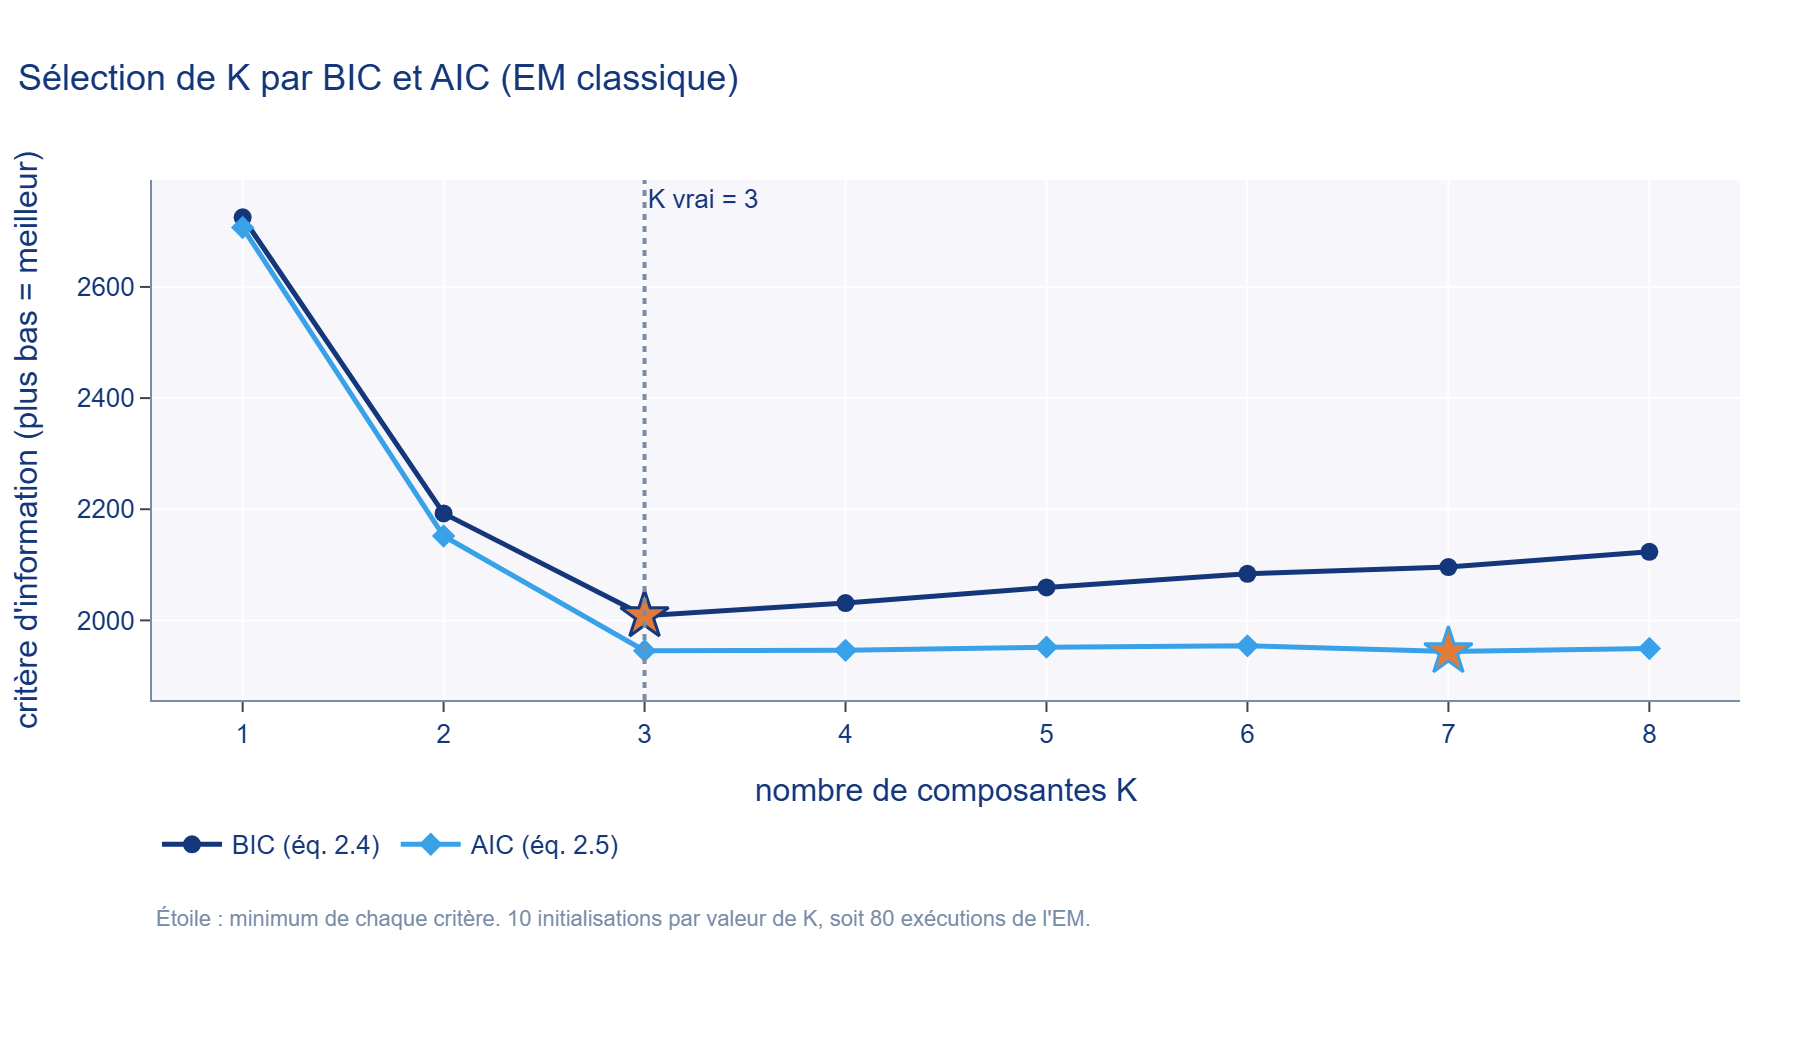
\includegraphics[width=0.85\textwidth]{figures/fig02.png}
\caption{Critères BIC et AIC de l'EM classique en fonction du nombre de composantes K, sur le jeu de données à trois groupes réels.}
\label{fig:2_1}
\end{figure}
Les deux critères atteignent leur minimum à $K = 3$ (valeur réelle) sur ce jeu, de sorte que la sélection externe par BIC ou AIC fonctionne lorsqu'elle est appliquée avec soin. Cette figure fixe la \emph{baseline pertinente} pour la suite : la comparaison utile n'est pas « EM avec $K = 6$ imposé contre VB avec $K_{\max} = 6$ » (situation volontairement défavorable à l'EM, section 2.3.7), mais « EM avec $K$ choisi par BIC ou ICL contre VB ». Le coût de cette baseline (un ajustement EM par valeur de $K$ et par initialisation) est comparé au coût d'un ajustement variationnel en temps total, jamais en proportion du nombre de valeurs de $K$ testées.

\section{Étude expérimentale}
\subsection{Protocole expérimental}
Afin d'illustrer concrètement les différences de comportement entre l'EM classique et l'EM variationnel mises en évidence sur le plan théorique, nous avons conduit une étude expérimentale fondée sur un jeu de données synthétique bidimensionnel. Ce choix méthodologique permet une visualisation directe des résultats et une interprétation sans ambiguïté des mécanismes en jeu.

Le jeu de données est constitué de N = 300 observations bidimensionnelles, générées à partir de trois groupes gaussiens, de centres respectifs (0, 0), (5, 5) et (0, 5), chacun comportant 100 observations et une covariance isotrope d'écart-type 0,7 (variance 0,49). Les centres sont distants de 5 à 7,1 unités, soit de 7 à 10 écarts-types : les trois groupes sont donc bien séparés. Ce jeu de données constitue, par construction, un mélange à trois composantes gaussiennes. Il est tiré avec la graine 42 ; la section 2.3.13 répète le protocole sur trente jeux indépendants.

L'expérience consiste à ajuster, sur ce même jeu de données, un GMM classique via l'algorithme EM classique et un GMM bayésien via l'algorithme EM variationnel, en imposant dans les deux cas un nombre de composantes délibérément surestimé, K = 6, soit le double du nombre réel de groupes. L'objectif est d'observer comment chacun des deux algorithmes gère cette surestimation. Deux jeux d'hyperparamètres sont considérés pour l'EM variationnel : des priors empiriques (centrés sur les données : $\beta _{0}$ = 1, $W_{0}^{-1}$ égale à la covariance empirique) et des priors diffus ($\beta _{0}$ = $10^{-3}$, $W_{0}$ = I). Sauf mention contraire, les résultats rapportés utilisent les priors empiriques.

\begin{table}[H]
\centering
\small
\setlength{\tabcolsep}{0.14cm}
\begin{tabular}{|p{7.42cm}|p{7.42cm}|}
\hline
\textbf{Paramètre} & \textbf{Valeur} \\
\hline
Nombre d'observations (N) & 300 (3 groupes de 100) \\
\hline
Dimension (D) & 2 \\
\hline
Nombre de composantes imposé (K) & 6 (nombre réel de groupes : 3) \\
\hline
Covariance des groupes générateurs & Isotrope, écart-type 0,7 (variance 0,49) \\
\hline
Graine de génération des données & 42 \\
\hline
EM classique & Mélange gaussien, covariance pleine, initialisation par k-means \\
\hline
EM variationnel & GMM bayésien, covariance pleine, prior de Dirichlet fini de concentration $\alpha _{0}$ \\
\hline
Priors Normal-Wishart (« empiriques », Bayes empirique) & $m_{0}$ = moyenne des données, $\beta _{0}$ = 1, $\nu _{0}$ = D, $W_{0}^{-1}$ = covariance empirique : les données servent deux fois (priors et vraisemblance) \\
\hline
Concentration du prior de Dirichlet ($\alpha _{0}$) & 1 / K = 0,167 \\
\hline
Critère d'arrêt & Identique pour tous les algorithmes : variation relative du critère total $\leq 10^{-6}$ (log-vraisemblance pour l'EM et le MAP-EM, ELBO pour le VB en covariance pleine) \\
\hline
Nombre maximal d'itérations & 500 étapes M pour tous les algorithmes ; une exécution qui atteint le plafond est marquée « non convergée » \\
\hline
Nombre d'initialisations & 10 (meilleur critère retenu) \\
\hline
Composante active & $N_k \geq 1$ (convention historique, sensibilité mesurée au tableau~\ref{tab:S10}) et $N_k/N \geq 1\,\%$ dans les scénarios \\
\hline
\end{tabular}
\caption{Paramètres du protocole expérimental}
\label{tab:2_4}
\end{table}
\emph{Source : implémentation PyTorch décrite à l'annexe A.}

\begin{figure}[H]
\centering
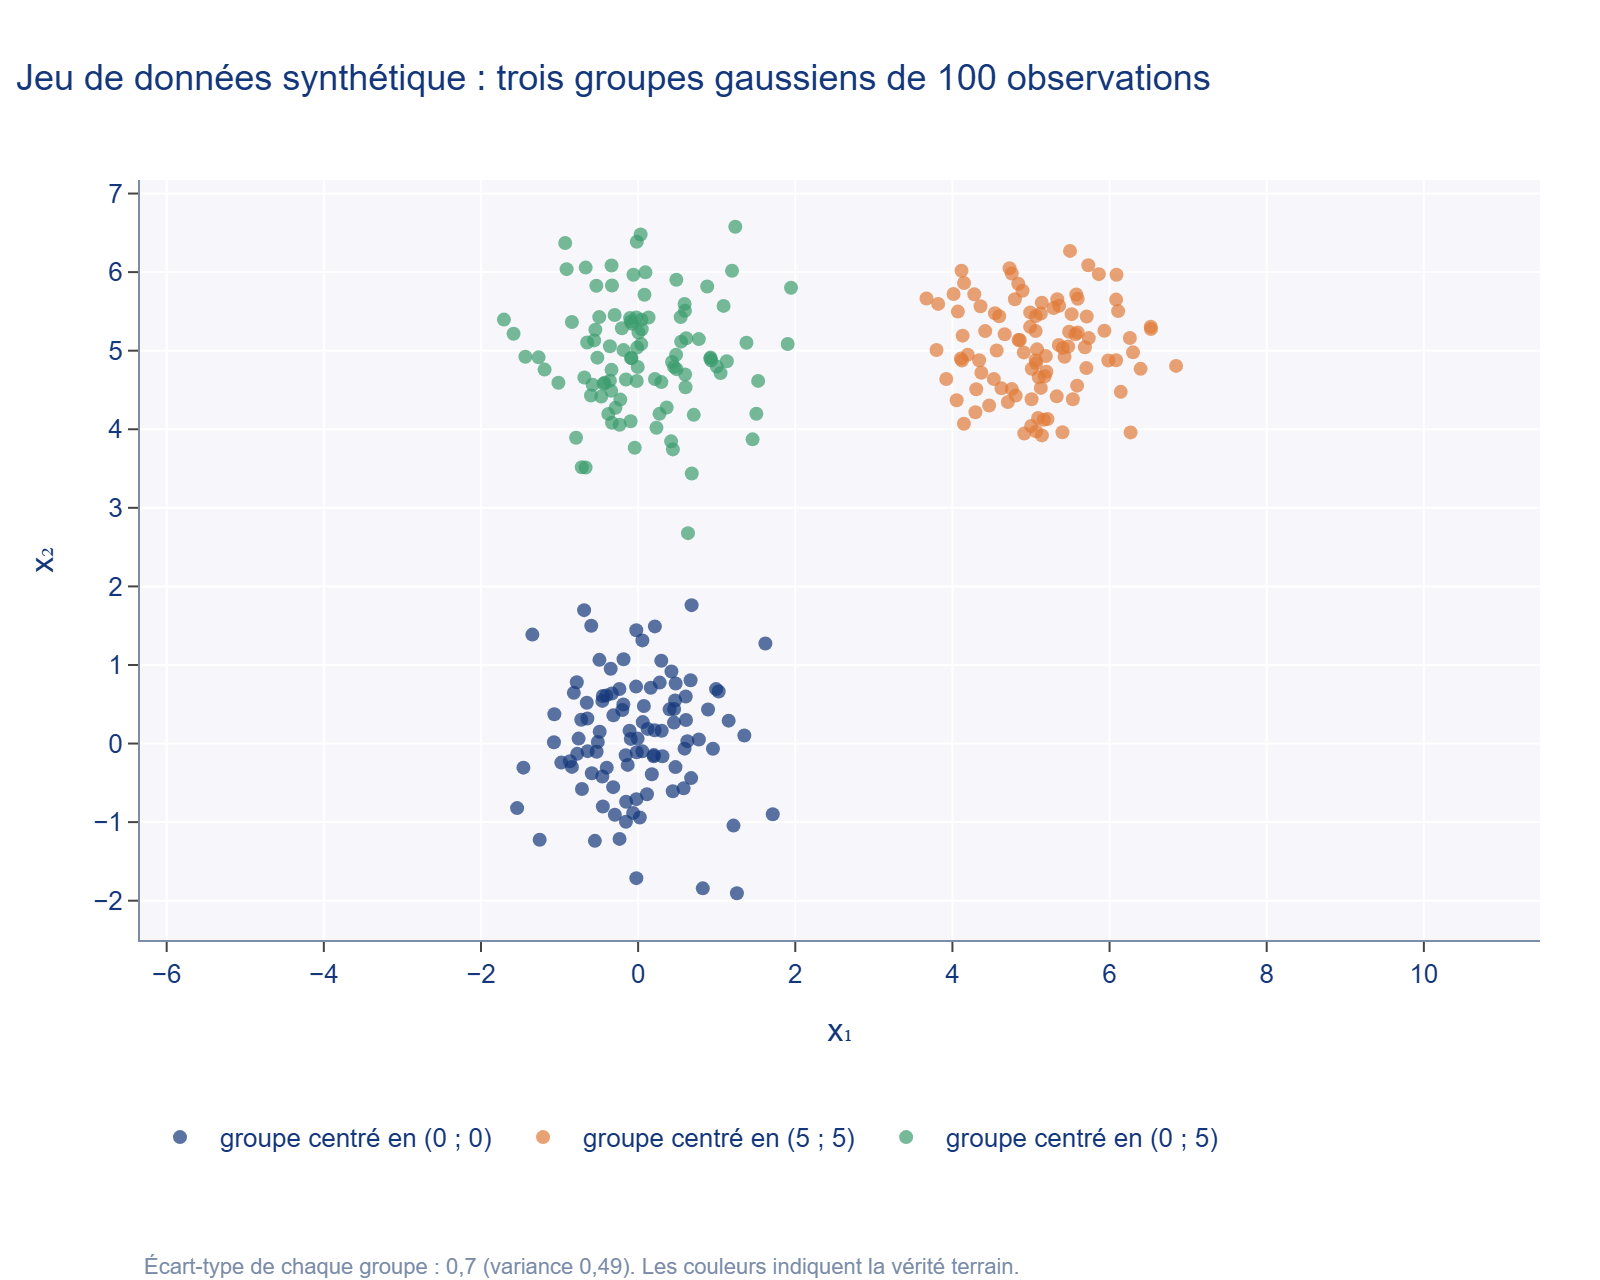
\includegraphics[width=0.85\textwidth]{figures/fig03.png}
\caption{Jeu de données synthétique utilisé pour l'étude expérimentale : trois groupes gaussiens réels de 100 observations chacun (N = 300 au total).}
\label{fig:2_2}
\end{figure}
\subsection{Résultats de l'EM classique (K = 6 imposé)}
L'EM classique est ajusté avec $K=6$ composantes (dix initialisations, critère d'arrêt commun) ; le nombre d'itérations, l'indicateur de convergence et l'indicateur de dégénérescence figurent au tableau~\ref{tab:2_7}. Le tableau~\ref{tab:2_5} présente les poids finaux obtenus pour chacune des six composantes.

\tableauGenere{poids_em}
Ce résultat illustre la limite décrite au chapitre 1 : en l'absence de mécanisme de régularisation sur le nombre de composantes, l'EM classique conserve ses six composantes. Aucun poids ne tombe sous le seuil d'activité $N_k = 1$ : aucune composante n'est écartée. Une composante de poids voisin d'un tiers capture à elle seule l'un des trois groupes, tandis que les autres se partagent les deux groupes restants, pourtant bien séparés, en les fragmentant (figure~\ref{fig:2_3}). Cette fragmentation est la source de l'ARI plus faible de l'EM à $K=6$ : elle mesure ce que font les composantes excédentaires, non un défaut intrinsèque de l'algorithme (section 2.3.12). L'EM n'a aucun mécanisme interne pour reconnaître que $K=6$ est surestimé, mais un balayage de $K$ par BIC ou ICL le fait (section 2.2.3), ce que compare la section 2.3.16.

\subsection{Résultats de l'EM variationnel (Kmax = 6)}
L'EM variationnel est ajusté avec $K_{\max}=6$, des priors empiriques et un prior de Dirichlet de concentration $\alpha_0 = 1/K$ ; l'ELBO est calculée exactement selon l'équation (1.31). Sa valeur finale (figure~\ref{fig:2_7}) est inférieure à la log-vraisemblance maximale de l'EM classique, comme l'exige la chaîne d'inégalités $\mathrm{ELBO} \leq \log p(X) \leq \max_{\theta} \log p(X \mid \theta)$ : les deux quantités ne mesurent pas la même chose (l'ELBO intègre la pénalité de complexité due aux priors) et ne se comparent pas comme deux scores d'ajustement. Le tableau~\ref{tab:2_6} présente les poids finaux obtenus.

\tableauGenere{poids_vb}
Contrairement à l'EM classique, l'EM variationnel identifie trois composantes dominantes de poids proches d'un tiers, la proportion réelle de chaque groupe, tandis que les trois autres voient leur poids s'effondrer sous le seuil d'activité $N_k < 1$ défini à la section 1.7.4. Elles sont éteintes (mécanisme de la section 1.7.4, via $\mathbb{E}[\log\pi_k]$) et le modèle final conserve trois composantes actives. Cet élagage ne se produit toutefois que pour des priors adaptés à l'échelle des données (ci-dessous) et dépend de $K_{\max}$ : le VB n'est pas libéré du choix de $K$, il le déplace vers $K_{\max}$ et les hyperparamètres. La figure~\ref{fig:2_3} illustre le contraste : les ellipses de l'EM classique se répartissent de façon désordonnée sur deux des groupes, celles du VB épousent les trois groupes.

Ce résultat dépend des priors. Avec les priors diffus ($\beta_0 = 10^{-3}$, $W_0 = I$), la même expérience conserve une composante active supplémentaire de faible poids et un ARI légèrement inférieur (tableau~\ref{tab:2_7}), avec davantage d'itérations. La section 2.3.13 mesure cette dépendance sur trente jeux d'un même générateur, et la section 2.3.19 par un plan factoriel sur les priors.

\begin{figure}[H]
\centering
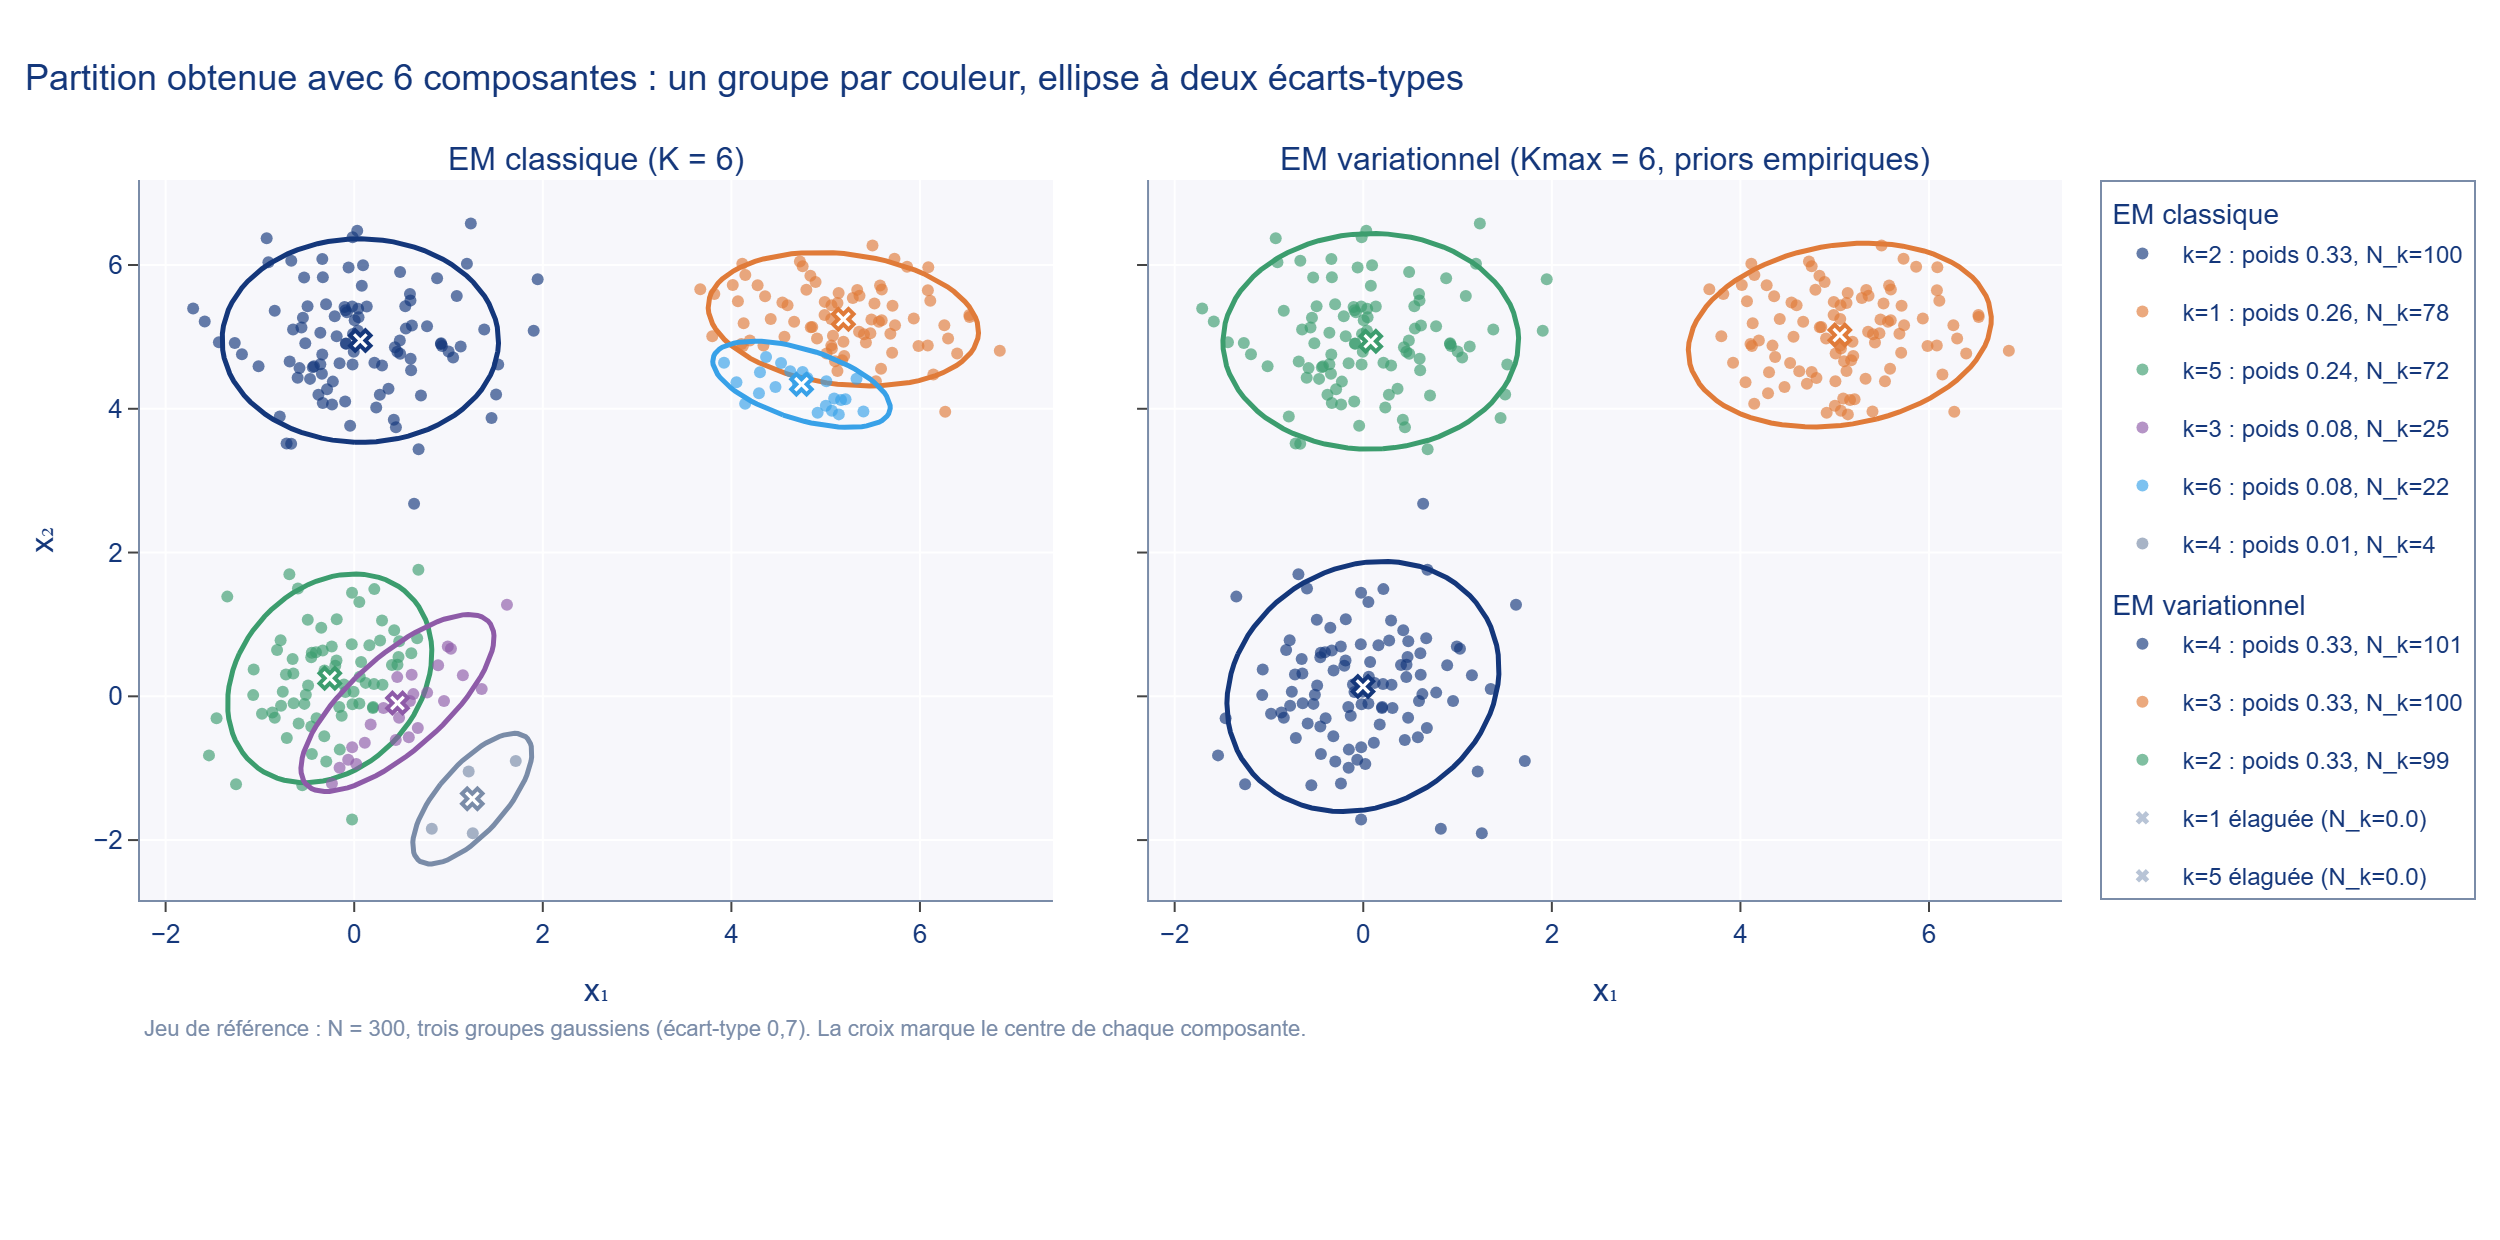
\includegraphics[width=0.95\textwidth]{figures/fig04.png}
\caption{Partition obtenue avec six composantes : une couleur par composante, ellipses de covariance à deux écarts-types, croix aux centres. À gauche, l'EM classique conserve ses six composantes ; à droite, l'EM variationnel n'en retient que trois (les composantes élaguées figurent en gris dans la légende).}
\label{fig:2_3}
\end{figure}
\begin{figure}[H]
\centering
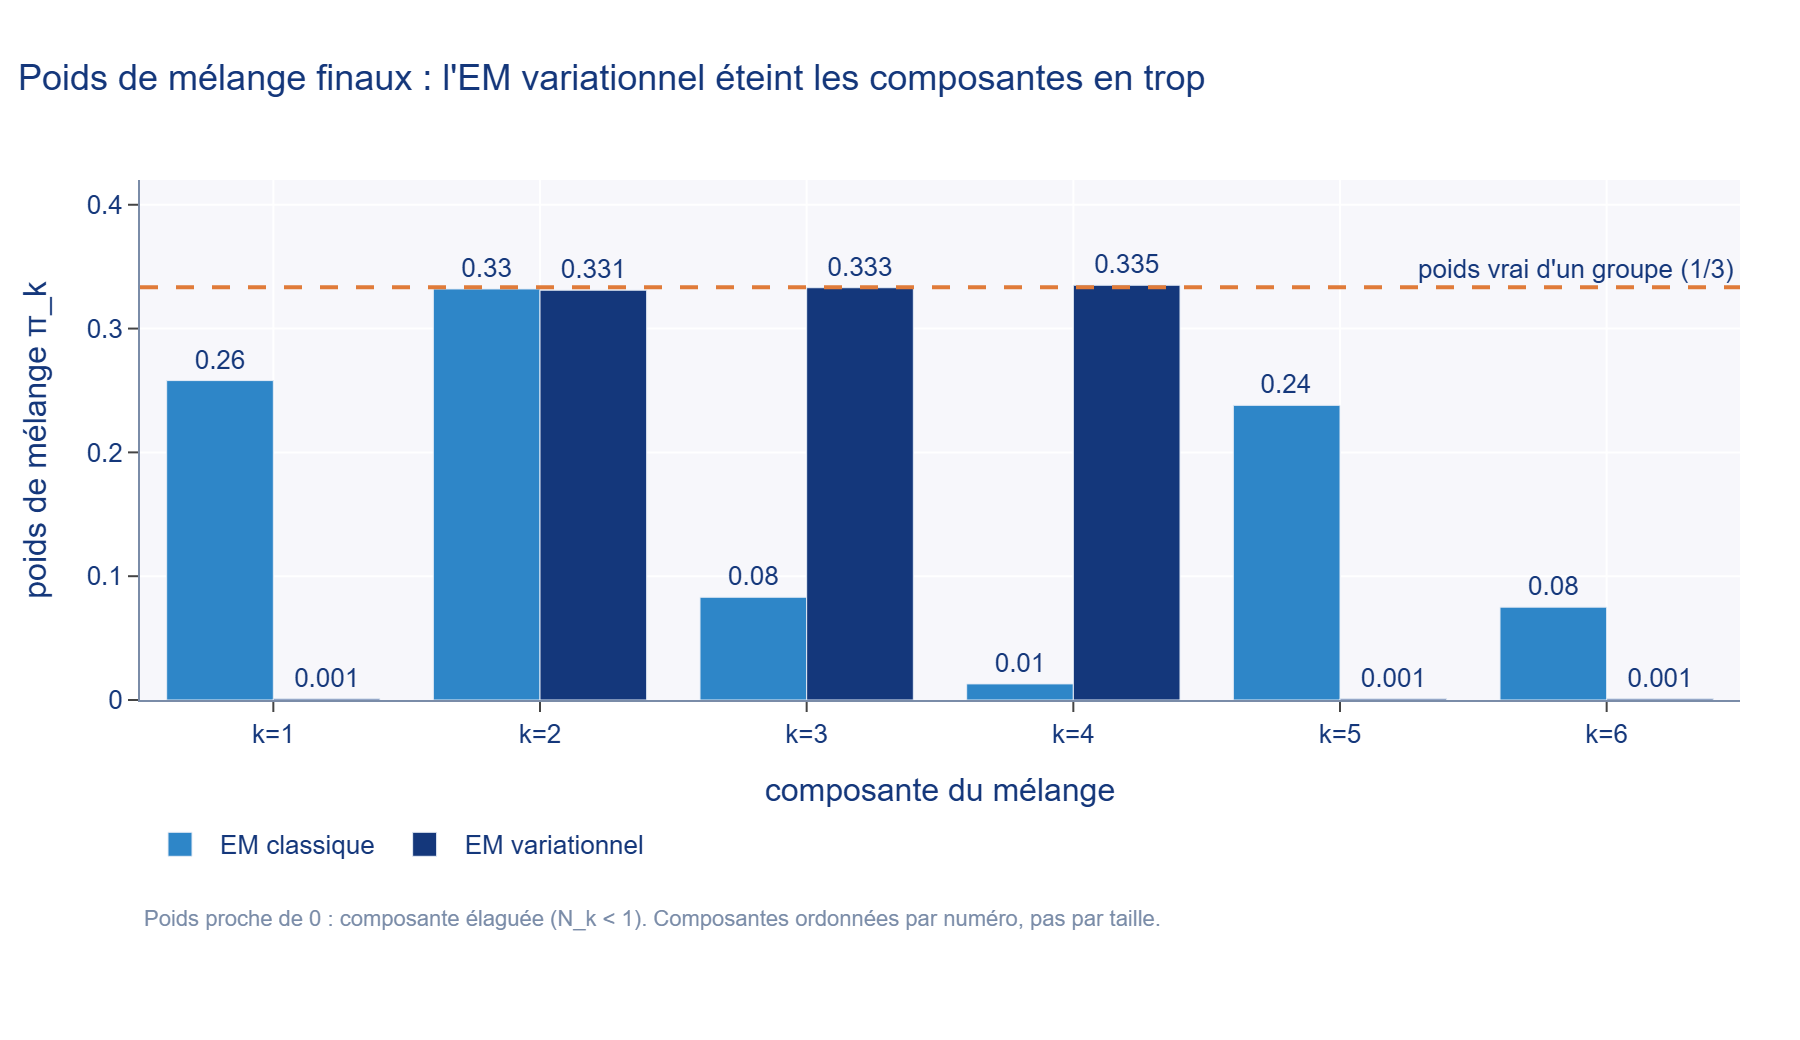
\includegraphics[width=0.85\textwidth]{figures/fig05.png}
\caption{Poids de mélange $\pi _{k}$ finaux pour les six composantes : EM classique et EM variationnel. Le contraste traduit le mécanisme d'élagage bayésien décrit à la section 1.7.4.}
\label{fig:2_4}
\end{figure}
\subsection{Comparaison visuelle et qualité de partition}
Au-delà des poids de mélange, la qualité des partitions obtenues par les deux algorithmes peut être évaluée à l'aide de métriques externes de clustering, en comparant les affectations produites aux véritables étiquettes de groupe. Le tableau 2.7 présente les résultats obtenus pour l'indice de Rand ajusté (ARI) et le score de silhouette, calculés sur les affectations dures obtenues en prenant, pour chaque observation, la composante de responsabilité maximale.

\tableauGenere{t2_7}
\emph{Source : implémentation PyTorch (graine 42). Les temps sont des moyennes sur les 30 jeux de la section 2.3.13.}

Ces résultats appellent quatre commentaires (tableau~\ref{tab:2_7}). Premièrement, l'ARI du VB à priors empiriques est supérieur à celui de l'EM à $K=6$ : la partition du VB est proche des trois groupes générateurs, celle de l'EM à $K=6$ est fragmentée. Cette comparaison est toutefois défavorable à l'EM par construction ($K=6$ imposé) ; la comparaison pertinente est avec EM-BIC et EM-ICL (section 2.3.16). Deuxièmement, la silhouette n'est pas comparable entre des solutions de nombres de composantes différents : elle mesure surtout ce nombre, et n'est donc pas utilisée comme preuve. Troisièmement, avec le \emph{même} critère d'arrêt, le nombre d'itérations du VB à priors empiriques n'est pas supérieur à celui de l'EM à $K=6$ ; le constat antérieur d'un VB environ trois fois plus long provenait d'une asymétrie de normalisation du critère (par observation pour l'EM, totale pour le VB), et non d'une propriété des algorithmes. L'EM à composantes fragmentées et fortement chevauchantes converge lentement (taux linéaire proche de 1, section 1.6.3.b), ce que le tableau est compatible avec, sans l'établir. Quatrièmement, le temps total dépend aussi du nombre d'initialisations et de l'implémentation : il n'est comparé qu'à critère et machine communs (sections 2.3.6 et 2.3.19).

\subsection{Sensibilité au choix du prior de Dirichlet ($\alpha _{0}$)}
La section 1.7.4 a montré que la concentration $\alpha_0$ du prior de Dirichlet contrôle l'élagage. Pour le vérifier, l'expérience de la section 2.3.3 est répétée en faisant varier $\alpha_0$ sur la grille $\{0{,}001;\,0{,}01;\,0{,}1;\,1;\,10\}$, toutes choses égales par ailleurs ($K_{\max}=6$, mêmes données, dix initialisations), pour les deux jeux de priors (tableau~\ref{tab:2_8}, figure~\ref{fig:2_5}). Cette grille est grossière autour de la zone de transition : la section 2.3.14 la complète.

\tableauGenere{t2_8}
\begin{figure}[H]
\centering
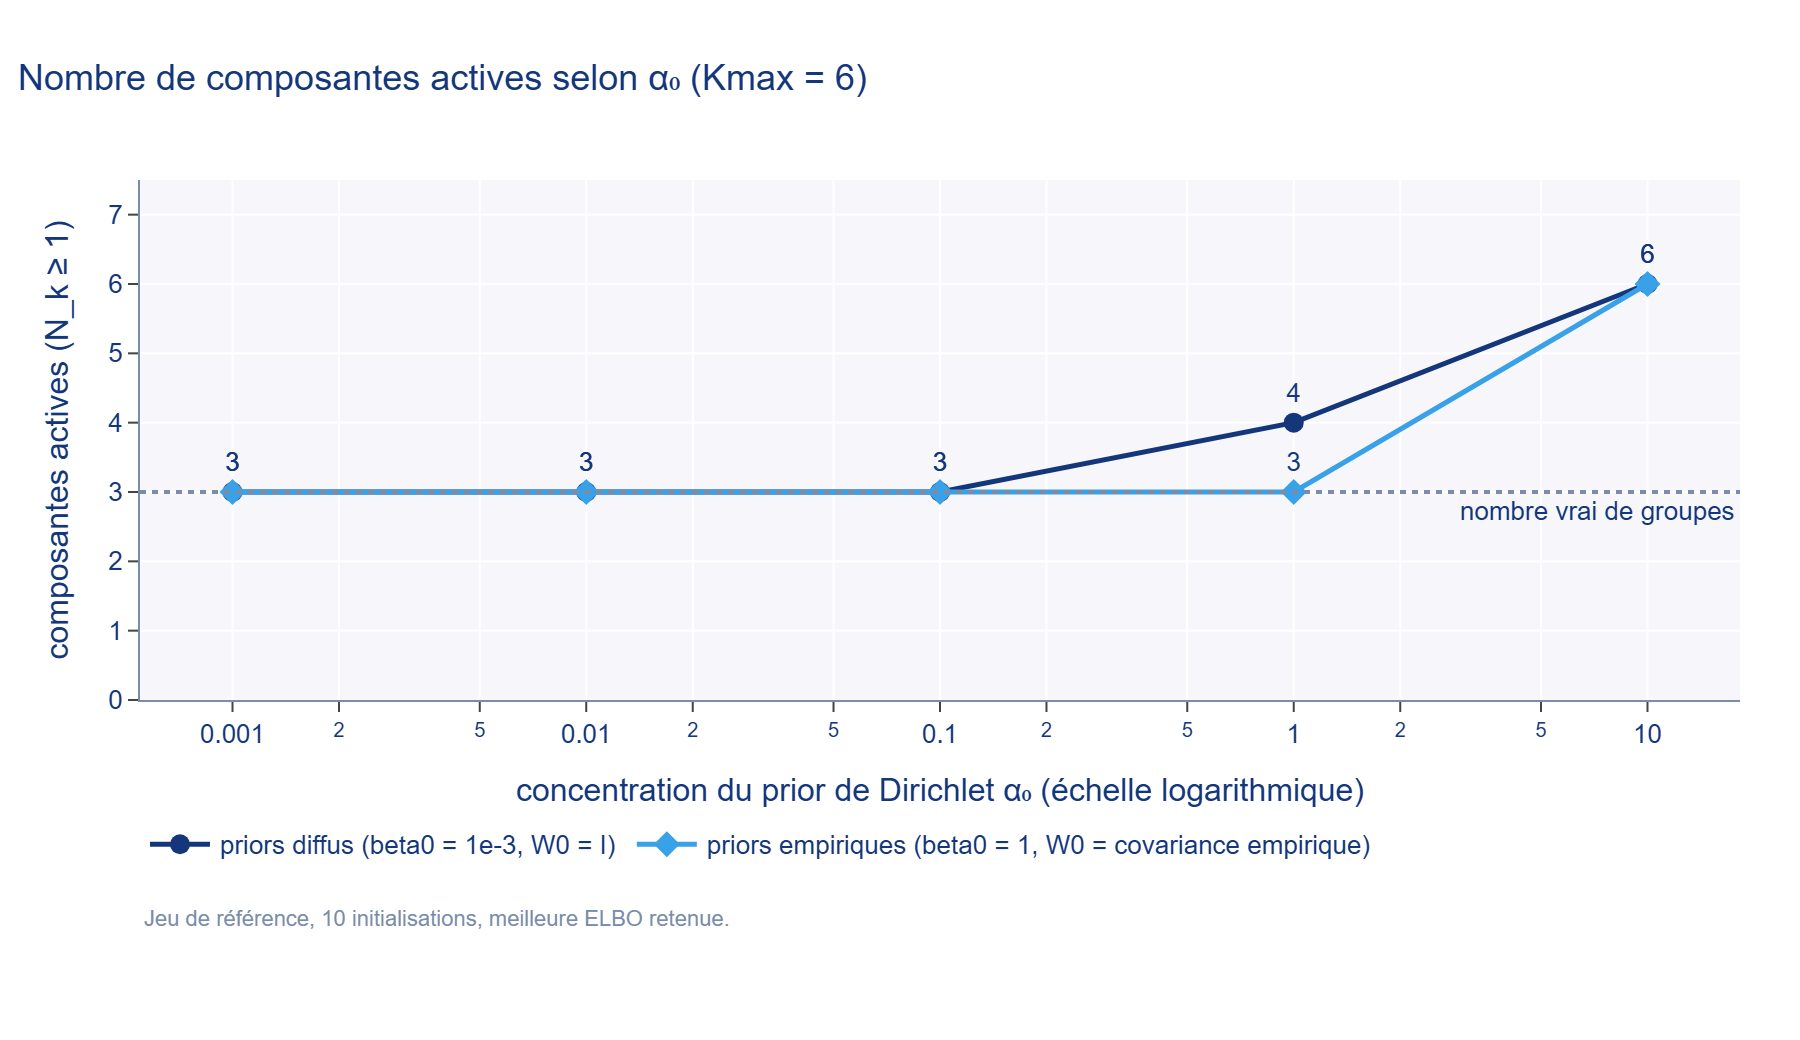
\includegraphics[width=0.85\textwidth]{figures/fig06.png}
\caption{Nombre de composantes actives en fonction de la concentration $\alpha _{0}$ du prior de Dirichlet (échelle logarithmique), pour les deux jeux de priors. Le mécanisme d'élagage disparaît lorsque $\alpha _{0}$ devient grand.}
\label{fig:2_5}
\end{figure}
Pour $\alpha_0 \leq 0{,}1$, le VB identifie trois composantes actives avec les deux jeux de priors. À $\alpha_0 = 10$, les six composantes redeviennent actives ; la partition se dégrade nettement avec les priors diffus, beaucoup moins avec les priors empiriques (tableau~\ref{tab:2_8}). Ce dernier cas est instructif : avec six composantes actives (au seuil $N_k \geq 1$), l'ARI reste élevé, de sorte que le nombre de composantes actives n'est pas une mesure fiable de la qualité de la partition ; il reflète que des composantes peu pondérées subsistent sans fragmenter les gros groupes, et dépend du seuil (section 2.3.19). À $\alpha_0 = 1$, l'élagage persiste, ce qui est compatible avec le seuil $d/2 = 2{,}5$ de Rousseau et Mengersen (2011) pour une covariance pleine en dimension 2 : on est en deçà du seuil. Cette lecture reste une hypothèse, la théorie portant sur le posterior exact et non sur le champ moyen ; la grille de la section 2.3.14 la teste autour du seuil. En pratique, $\alpha_0$ est un levier de parcimonie, mais le déplacement de la sensibilité de $K$ vers $(\alpha_0, \beta_0, \nu_0, W_0)$ est un inconvénient du VB, à inscrire dans la grille de synthèse.

\subsection{Étude de la scalabilité computationnelle}
Pour quantifier le surcoût de l'EM variationnel identifié à la section 2.2.1, le temps d'exécution des deux algorithmes est mesuré en faisant varier le nombre d'observations $N$ (à $D=2$) et la dimension $D$ (à $N=2000$). Chaque configuration est répétée dix fois (médiane), avec une initialisation et le critère d'arrêt commun ; le tableau~\ref{tab:2_9} sépare le temps jusqu'au modèle final, le nombre d'itérations et le coût par itération. Tableau et figure~\ref{fig:2_6} sortent du même run.

\tableauGenere{t2_9}
\begin{figure}[H]
\centering
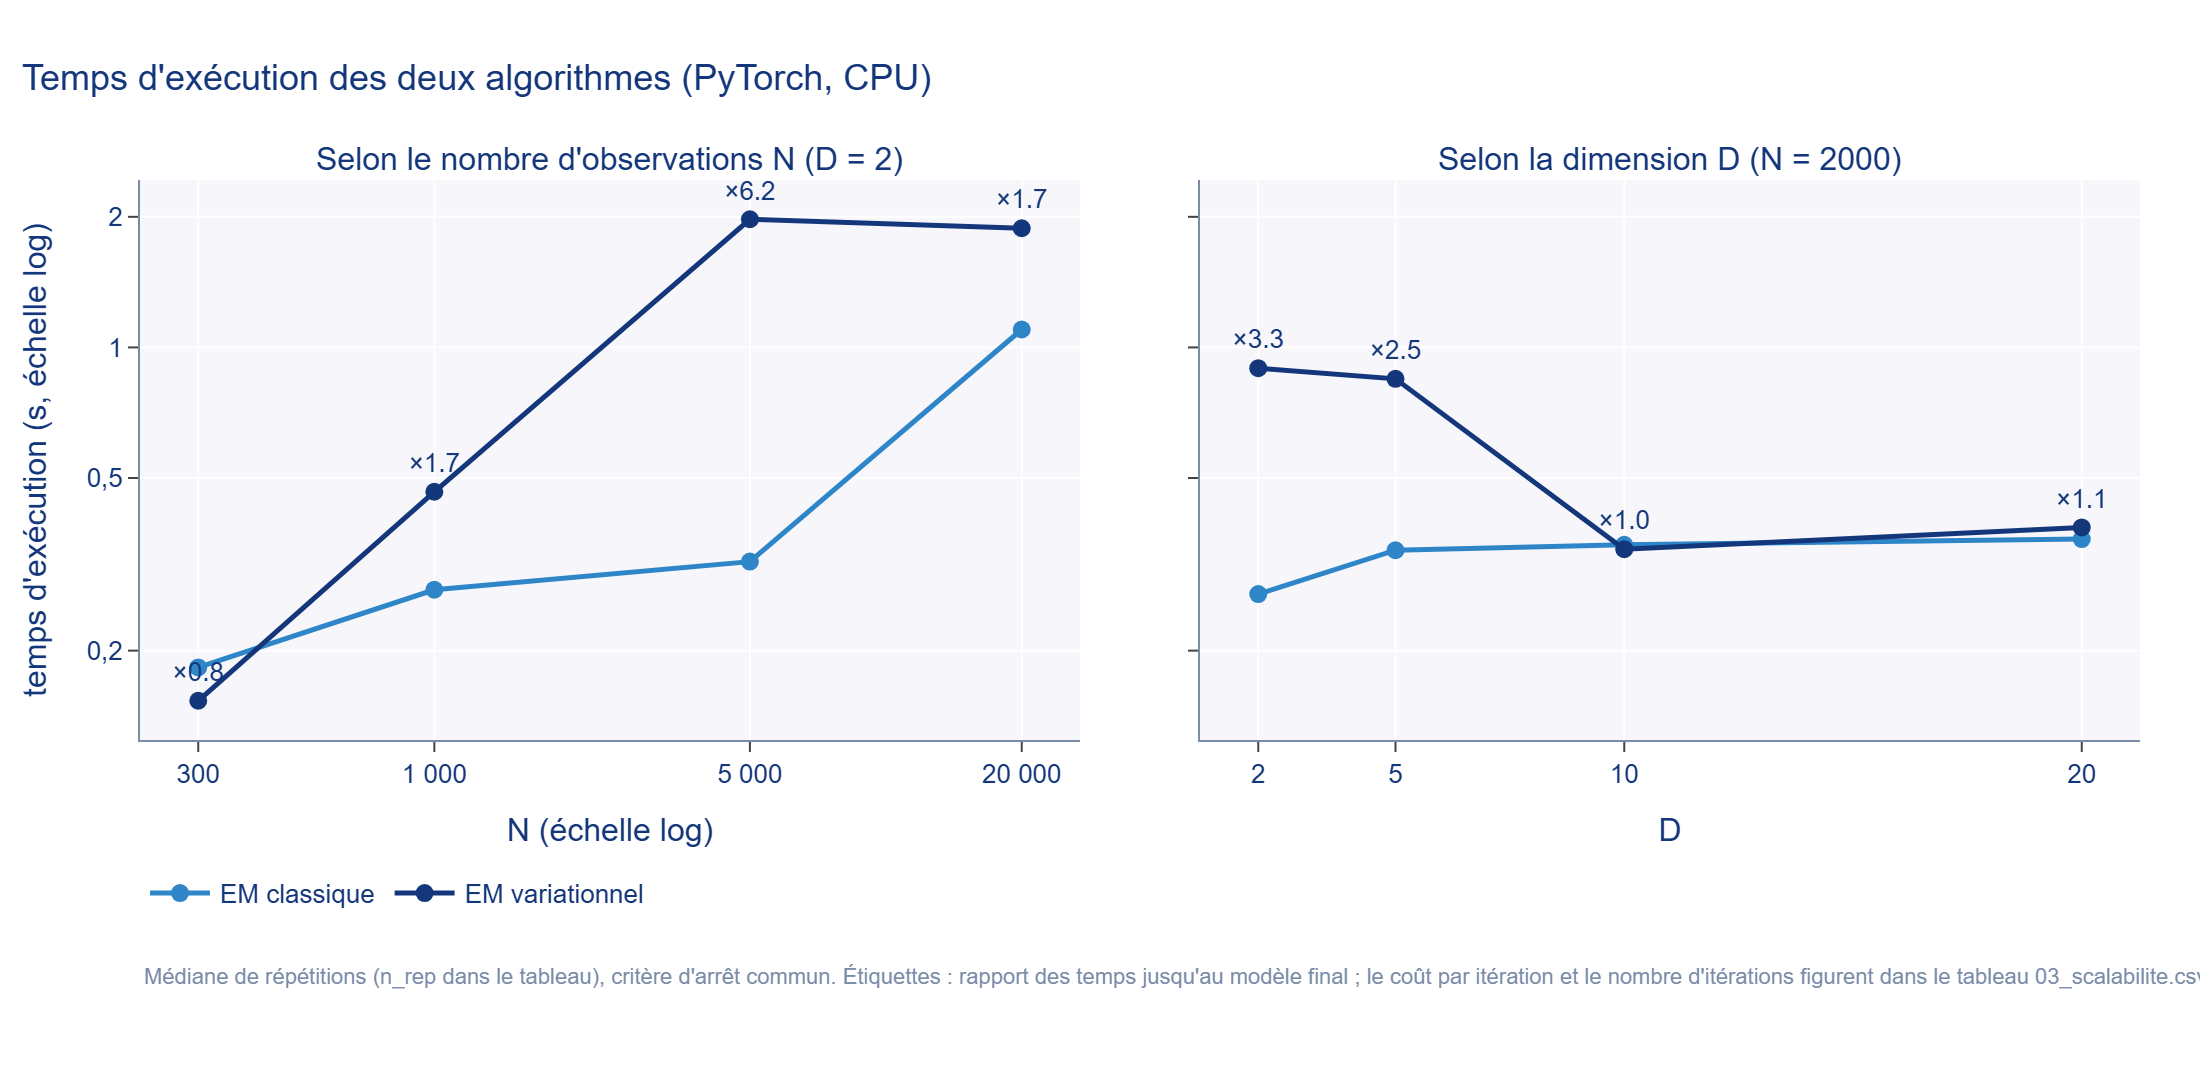
\includegraphics[width=0.95\textwidth]{figures/fig07.png}
\caption{Temps d'exécution des deux algorithmes en fonction du nombre d'observations N (à gauche, échelles logarithmiques) et de la dimension D (à droite). Les étiquettes donnent le rapport du temps variationnel au temps classique.}
\label{fig:2_6}
\end{figure}
\emph{Source : implémentation PyTorch (CPU, machine unique, graine 42).}

Les deux grandeurs doivent être lues séparément. Le \emph{coût par itération} du VB est supérieur à celui de l'EM d'un facteur de l'ordre de l'unité à quelques unités, sans tendance monotone nette en $N$ ni en $D$ (colonne « Ratio coût/itér. »). Le \emph{temps jusqu'au modèle final} est le produit de ce coût par le nombre d'itérations, qui varie d'une configuration à l'autre et dans un sens ou dans l'autre (colonnes « Itér. EM » et « Itér. VB ») : le ratio global ne se réduit donc ni à un facteur multiplicatif stable ni à l'analyse de complexité de la section 2.2.1, qui porte sur le coût par itération. Les mesures sont des médianes de dix répétitions, mais restent propres à une machine, à une implémentation et à des données synthétiques de $D \leq 20$. La conclusion « le VB est $x$ fois plus lent » n'est donc pas retenue ; la question utile, le temps total d'un pipeline EM-BIC contre un VB, est traitée à la section 2.3.19.

\subsection{Cas de référence : nombre de composantes correctement spécifié (K = 3)}
Les résultats précédents portent sur le cas, volontairement défavorable à l'EM classique, où le nombre de composantes est surestimé. Pour vérifier que les deux algorithmes se comportent de façon comparable en l'absence de cette surestimation, l'expérience est répétée avec $K = 3$, le nombre exact de groupes (tableau~\ref{tab:2_10}).

\tableauGenere{t2_10}
Lorsque le nombre de composantes est correctement spécifié, les deux algorithmes convergent vers des solutions quasi identiques (ARI et silhouette très proches, tableau~\ref{tab:2_10}) ; le petit écart d'ARI correspond vraisemblablement à une ou quelques observations de frontière, sans que ce point ait été identifié ni l'effet de régularisation des priors démontré. Le nombre d'itérations dépend de la tolérance relative commune appliquée à des critères d'échelles différentes (log-vraisemblance et ELBO) et ne se compare pas comme une propriété intrinsèque. Ce cas montre que l'avantage apparent du VB aux sections 2.3.3 et 2.3.4 tient à la surestimation imposée de $K$ ; il ne se manifeste pas lorsque $K$ est correct. Le choix entre les deux algorithmes ne peut donc pas s'appuyer sur ce seul contraste : il dépend de la confiance dans $K$, du besoin d'incertitude et du budget de calcul (grille du tableau~\ref{tab:2_17}).

\subsection{Convergence de l'ELBO}
La section 1.7.6 a établi que l'ELBO constitue, pour l'EM variationnel, un critère de convergence croissant et borné. La figure~\ref{fig:2_7} retrace l'évolution de l'ELBO, calculée exactement à chaque itération (équation 1.31) pour le modèle à $K_{\max}=6$ de la section 2.3.3 (même appel, donc même nombre d'itérations que le tableau~\ref{tab:2_7} : un seul décompte dans tout le mémoire), ainsi que la log-vraisemblance de l'EM classique à $K=6$.

\begin{figure}[H]
\centering
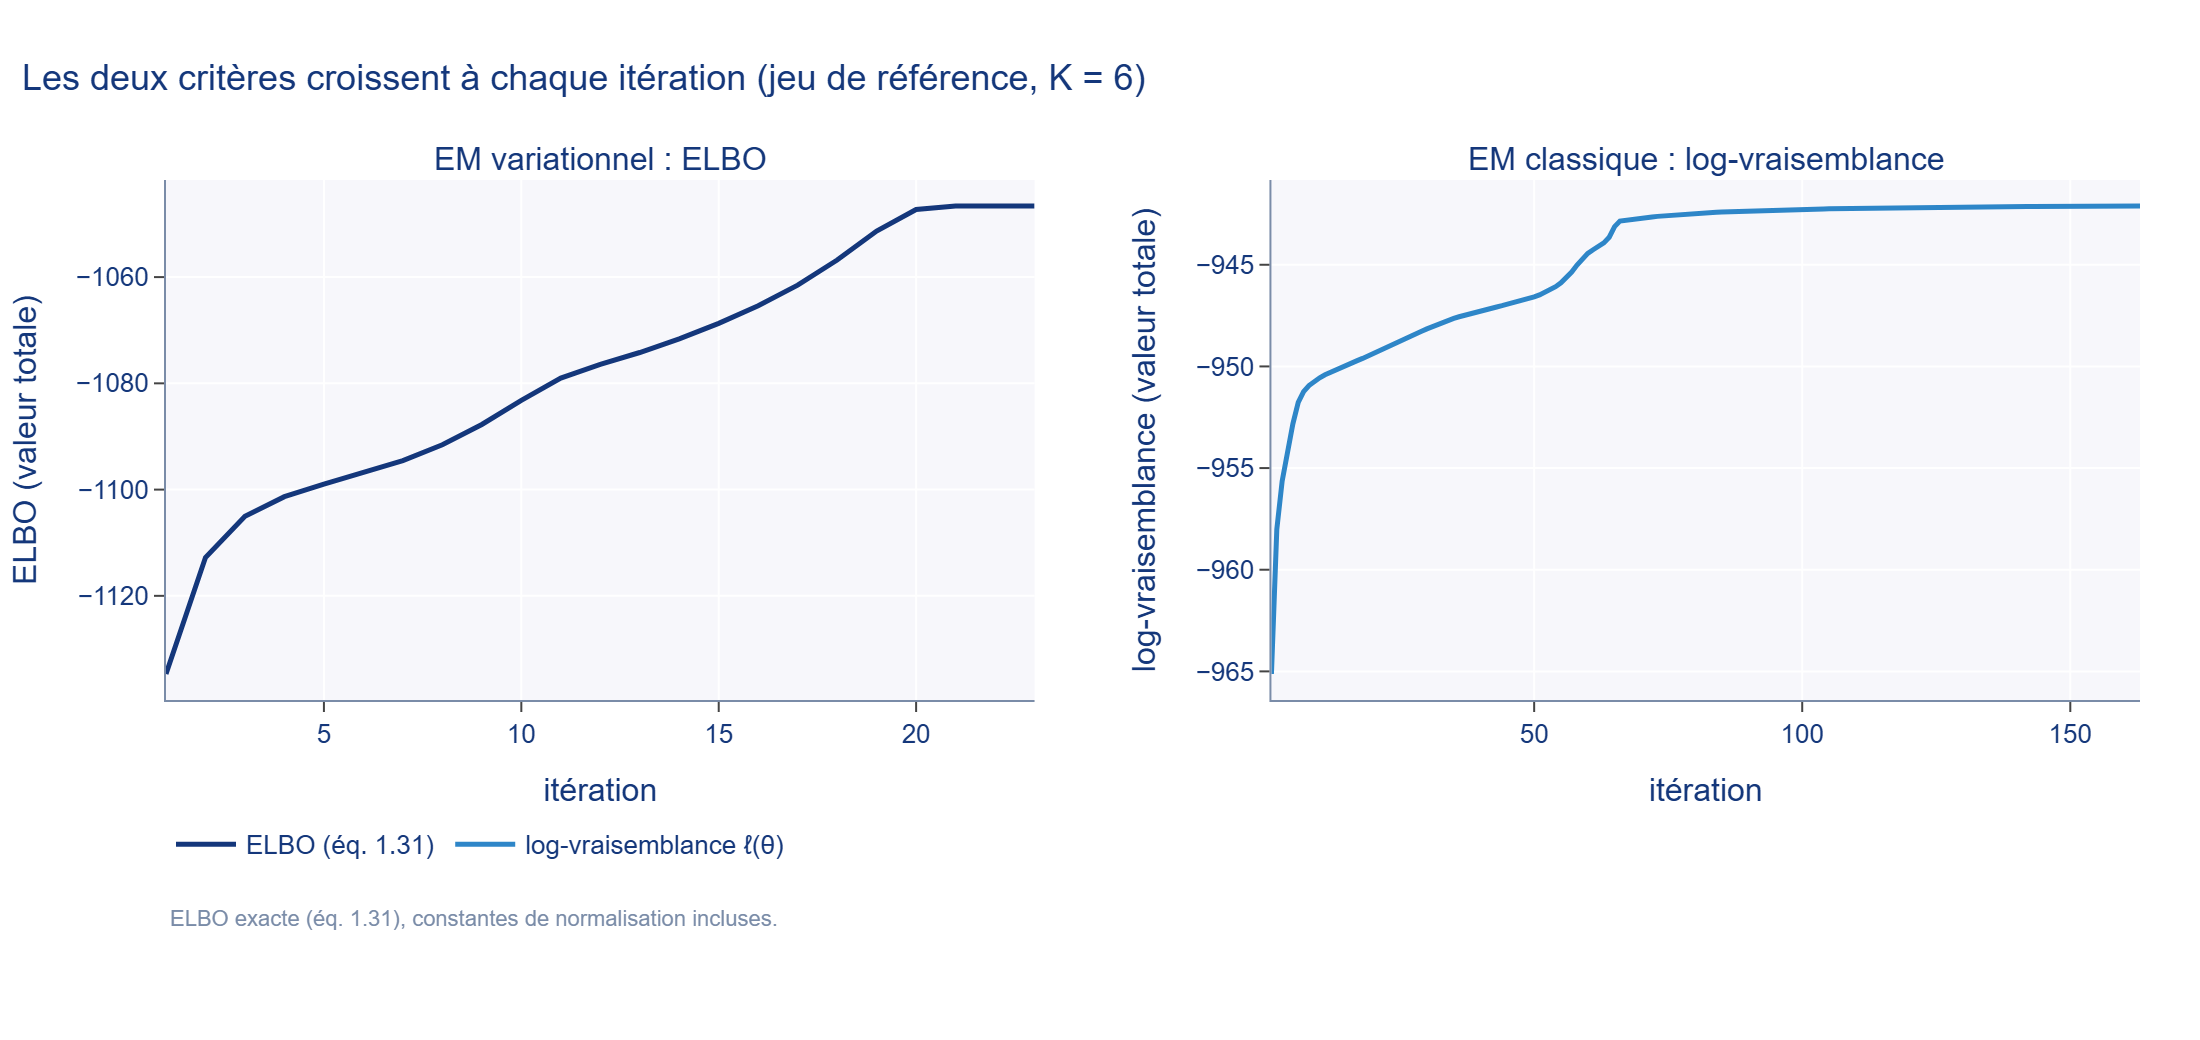
\includegraphics[width=0.95\textwidth]{figures/fig08.png}
\caption{Évolution de l'ELBO (EM variationnel, à gauche) et de la log-vraisemblance (EM classique, à droite) en fonction du nombre d'itérations. Les deux courbes sont croissantes, conformément aux garanties théoriques des sections 1.6.2.f et 1.7.6.}
\label{fig:2_7}
\end{figure}
L'ELBO croît strictement à chaque itération, conformément à la garantie de la section 1.7.6 ; cette monotonie, l'inégalité $\mathrm{ELBO} \leq \log p(X) \leq \ell(\hat\theta)$ et l'égalité de Neal et Hinton, $F(q^*, \theta) = \ell(\theta)$ après l'étape E, sont vérifiées numériquement par le code (journal d'exécution) et par des tests unitaires. L'ELBO gagne l'essentiel de son gain dans les premières itérations puis se stabilise. La courbe de log-vraisemblance de l'EM est tracée jusqu'à son critère d'arrêt, identique à celui du VB.

\subsection{Robustesse à l'initialisation}
Les résultats précédents ont été obtenus avec dix initialisations indépendantes, dont la meilleure est conservée (sections 1.6.3.a et 1.7.9). Pour mesurer la sensibilité propre de chaque algorithme, l'expérience de la section 2.3.1 est répétée avec une seule initialisation par exécution, pour 20 graines et deux stratégies : initialisation par k-means et initialisation aléatoire ($K$ points de données tirés au hasard, sections 1.6.2.a et 1.7.3.d).

\tableauGenere{t2_11}
\begin{figure}[H]
\centering
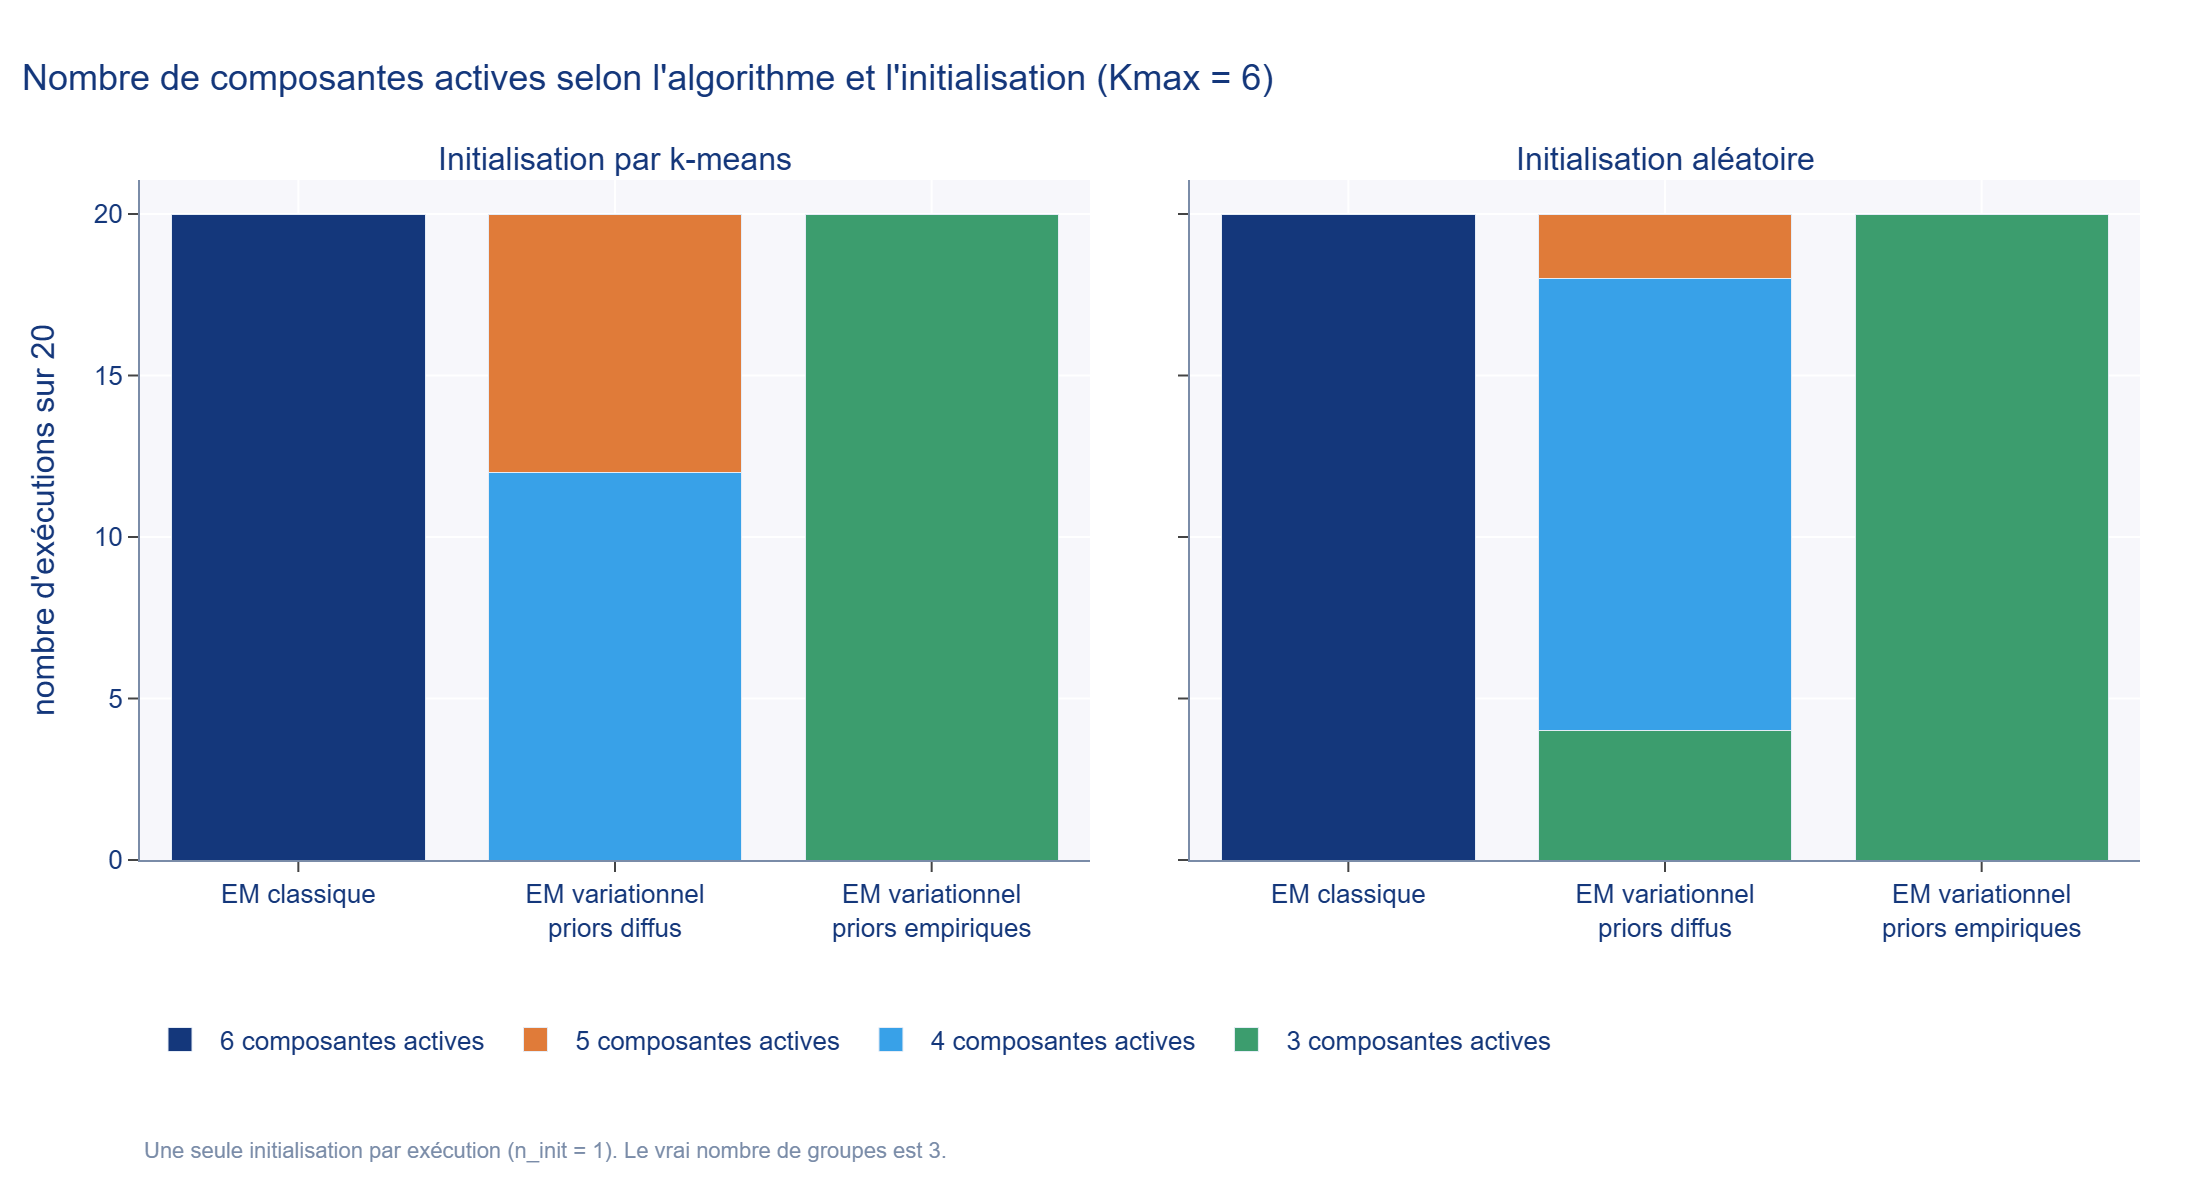
\includegraphics[width=0.95\textwidth]{figures/fig09.png}
\caption{Répartition du nombre de composantes actives selon l'algorithme et la stratégie d'initialisation (20 exécutions chacune, une initialisation par exécution).}
\label{fig:2_8}
\end{figure}
Avec les priors empiriques, l'EM variationnel retrouve trois composantes actives dans toutes les exécutions, quelle que soit la stratégie d'initialisation (tableau~\ref{tab:2_11}). Avec les priors diffus, le résultat dépend fortement de l'initialisation : trois composantes dans peu d'exécutions (initialisation aléatoire) ou aucune (k-means), les autres conservant quatre ou cinq composantes. L'EM classique conserve ses six composantes dans les exécutions du tableau : à $K$ fixé à 6, aucune initialisation ne lui permet de « reconnaître » que trois suffiraient, et ce résultat est trivial puisque rien n'élimine de composante. Le seul résultat informatif est donc celui du VB, et il est conditionnel : le VB est robuste à l'initialisation \emph{si} ses priors sont adaptés à l'échelle des données, et fragile sinon. Autrement dit, le VB déplace la sensibilité de l'initialisation vers les hyperparamètres ; c'est un inconvénient, inscrit comme tel dans le tableau~\ref{tab:2_17}.

\subsection{Sensibilité au type de covariance}
L'ensemble des expériences précédentes ont été conduites avec des matrices de covariance pleines (full), c'est-à-dire sans contrainte sur la forme des ellipses de covariance de chaque composante. En pratique, il est fréquent de contraindre cette forme, tant pour réduire le nombre de paramètres libres et le risque de surapprentissage que pour accélérer les calculs. Les quatre contraintes les plus courantes, par ordre décroissant de flexibilité, sont : full (une matrice pleine par composante), tied (une unique matrice pleine partagée par toutes les composantes), diag (une matrice diagonale par composante) et spherical (une variance scalaire par composante). Pour l'EM variationnel, les variantes tied, diag et spherical ne sont pas dérivées au chapitre 1 ; elles utilisent un prior de Wishart partagé (tied) ou des priors Gamma sur les précisions (diag, spherical), également conjugués. Le tableau 2.12 reproduit l'expérience de la section 2.3.4 pour chacune de ces contraintes.

\tableauGenere{t2_12}
\begin{figure}[H]
\centering
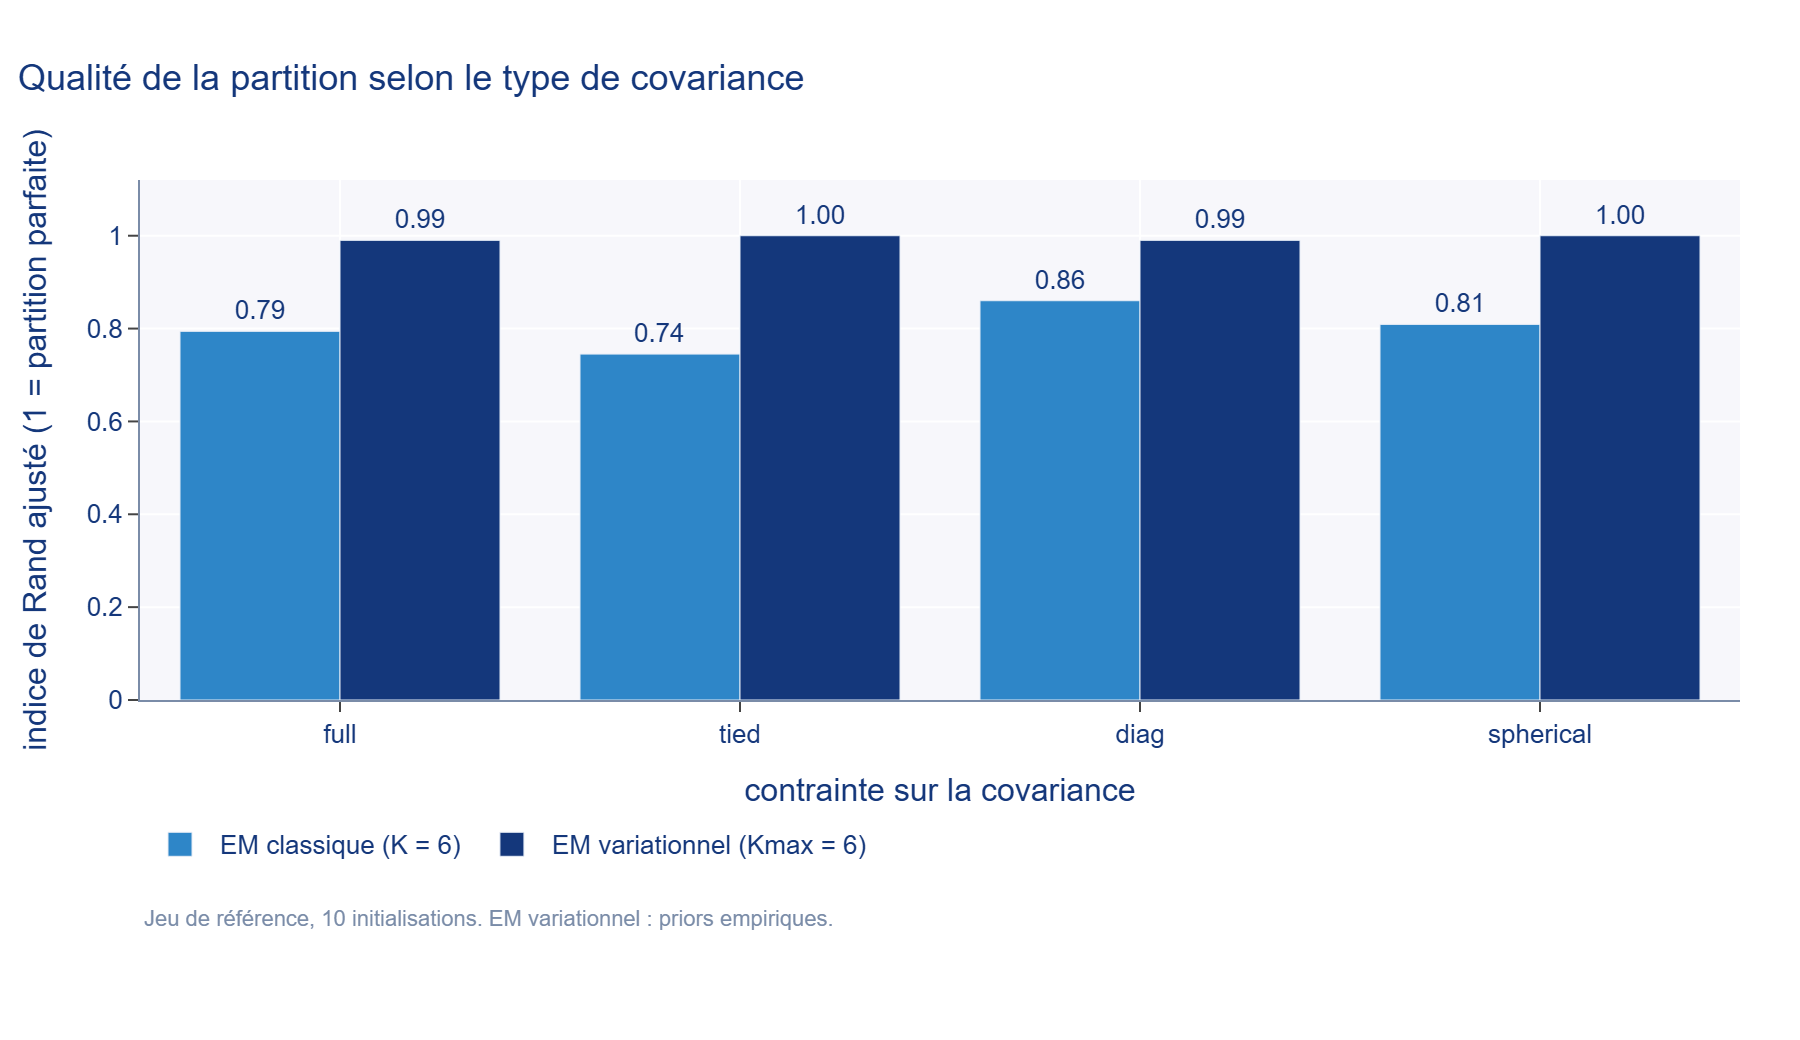
\includegraphics[width=0.85\textwidth]{figures/fig10.png}
\caption{Indice de Rand ajusté selon la contrainte imposée sur la covariance (K = 6 imposé).}
\label{fig:2_9}
\end{figure}
Dans les quatre cas, le VB conserve trois composantes actives avec un ARI proche de 1 (tableau~\ref{tab:2_12}) ; l'ARI de l'EM à $K=6$ reste inférieur et varie avec la contrainte. L'ARI de l'EM tied est inférieur à celui de l'EM full alors que les groupes sont isotropes : cette observation tient plus vraisemblablement à la fragmentation due à $K=6$ qu'à la forme de la covariance, sans que cela ait été analysé. Pour tied, diag et spherical, le VB utilise un critère d'arrêt approché (somme des log-normalisations de l'étape E, ELBO privé du terme KL sur $\theta$, non nécessairement monotone) et l'ELBO de ces variantes n'est pas dérivé : l'élagage est donc observé \emph{avec une approximation}. Il est plausible qu'il ne dépende pas de la forme de covariance, mais cette extension reste à valider en dérivant l'ELBO de chaque variante (section 3.3).

\subsection{Validation sur un jeu de données réel (Iris)}
Les résultats précédents ont été obtenus sur un jeu synthétique de trois groupes gaussiens séparés. Pour sortir de ce cadre idéalisé, l'expérience centrale est reproduite sur le jeu Iris de Fisher (1936) : $N=150$ observations en dimension $D=4$, trois espèces, mesures brutes en centimètres (non standardisées), avec $K=6$ imposé, puis $K=3$ (tableau~\ref{tab:2_13}).

\tableauGenere{t2_13}
\emph{Source : Iris de Fisher (1936), fichier UCI Machine Learning Repository ; calculs de l'auteur.}

\begin{figure}[H]
\centering
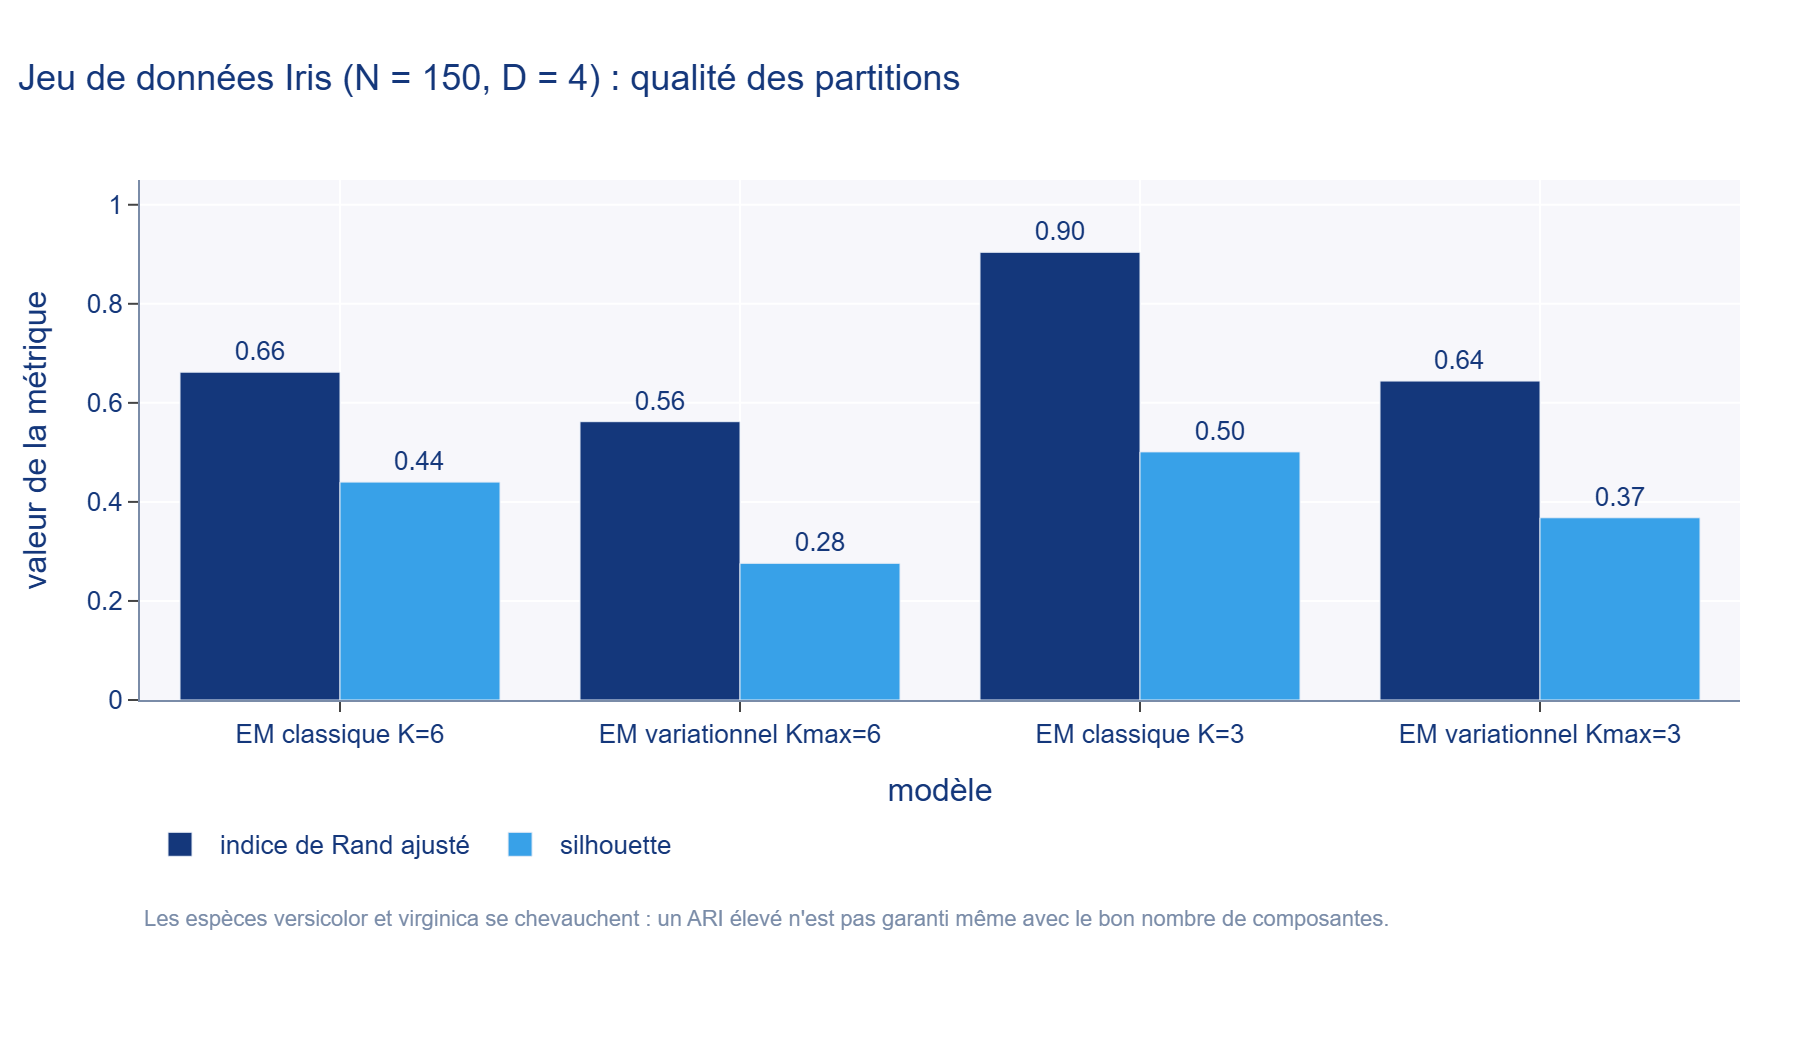
\includegraphics[width=0.85\textwidth]{figures/fig11.png}
\caption{Indice de Rand ajusté et silhouette sur le jeu Iris, selon l'algorithme et le nombre de composantes.}
\label{fig:2_10}
\end{figure}
Ce résultat obtenu sur données réelles nuance la section 2.3.4. À $K_{\max}=6$, le VB élague trois composantes mais son ARI est inférieur à celui de l'EM à $K=6$ (tableau~\ref{tab:2_13}). Les poids finaux en donnent la raison : une composante de poids voisin de 2/3 regroupe versicolor et virginica, et une composante de poids voisin de 1/3 isole setosa. L'élagage fusionne les deux espèces qui se chevauchent, ce qui est cohérent avec un support statistique insuffisant pour les séparer, alors que les étiquettes les distinguent. L'ARI n'est donc pas le bon juge ici ; la log-vraisemblance hors échantillon (validation croisée) et la comparaison avec EM-BIC, qui retient souvent $K=2$ sur Iris, seraient plus informatives (non testé ici). Un point de méthode : avec $N=150$, $D=4$ et $K=6$ en covariance pleine, l’EM compte environ 89 paramètres libres pour 150 points, cas typique de singularité ; l'indicateur de dégénérescence du tableau le signale pour l'EM à $K=6$, alors que la régularisation $\varepsilon I$ du code la masquait dans la version précédente de ce chapitre.

Avec $K_{\max}=3$, l'ARI du VB est supérieur à celui de $K_{\max}=6$ mais inférieur à celui de l'EM à $K=3$ exactement spécifié (tableau~\ref{tab:2_13}). Le résultat du VB dépend donc de $K_{\max}$ : à $K_{\max}=6$ il trouve deux grosses composantes, à $K_{\max}=3$ trois composantes de poids 0,16, 0,33 et 0,51 environ ; cela contredit l'idée que « $K_{\max}$ suffit » et confirme le déplacement de la sélection de $K$ vers $K_{\max}$. Sur ce jeu réel, si l'on a de bonnes raisons de croire que $K=3$, l'EM classique avec ce $K$ donne de meilleurs ARI que de compter sur l'élagage. Cette nuance, absente de l'étude synthétique, invite à ne pas généraliser les résultats obtenus sur des gaussiennes bien séparées.

\subsection{Sensibilité aux valeurs aberrantes}
Une dernière expérience examine le comportement des deux algorithmes en présence de valeurs aberrantes, situation fréquente en pratique et distincte de la simple surestimation de K. Dix points, tirés uniformément dans le carré $[-10 ; 15]^{2}$ (graine 7), ont été ajoutés au jeu de données de la section 2.3.1, puis les deux algorithmes ont été ajustés avec K = 6 sur ce jeu augmenté (N = 310).

\tableauGenere{t2_14}
Cette expérience, fondée sur un seul tirage (graine 7), n'est pas un test de robustesse : c'est une \emph{illustration d'un artefact de l'indicateur}. Avec $K = 6$ imposé, les composantes excédentaires de l'EM fragmentent les trois groupes réels sur données propres (ARI du tableau 2.7) ; en présence d'aberrations, elles sont absorbées par ces points isolés, et les trois groupes ne sont plus fragmentés. L'ARI hors aberrations remonte alors pour une raison qui tient à ce que font les composantes en trop, non à la qualité de l'algorithme. Il serait faux de lire dans le tableau 2.14 que « les deux algorithmes sont robustes » ou que le VB « absorbe mieux » les aberrations : la trace de sa composante diffuse est un résultat ambigu. Un test de robustesse exige au moins 30 tirages, des proportions et des amplitudes d'aberrations variées, et une comparaison avec la baseline EM-BIC (et, idéalement, une composante uniforme de fond) : c'est le scénario S7 de la section 2.3.18.

\subsection{Réplication sur 30 tirages d'un même générateur}
Les sections précédentes reposent sur un jeu de données unique. Pour chiffrer l'incertitude, le protocole de la section 2.3.1 ($K=6$ imposé, dix initialisations) est répété sur $R=30$ jeux d'un même générateur (graines 1000 à 1029). Trois hypothèses, fixées avant l'analyse, sont testées : (H1) l'ARI moyen du VB dépasse celui de l'EM, décidé si l'intervalle bootstrap à 95 \% de la différence appariée est strictement positif ; (H2) le VB retrouve exactement trois composantes actives dans la majorité des jeux, décidé si la borne basse de l'intervalle de Wilson à 95 \% dépasse 0,5 ; (H3) ces résultats dépendent du choix des priors. Résultats : tableaux~\ref{tab:2_15} et~\ref{tab:2_16}.

\tableauGenere{t2_15}
\tableauGenere{t2_16}
\begin{figure}[H]
\centering
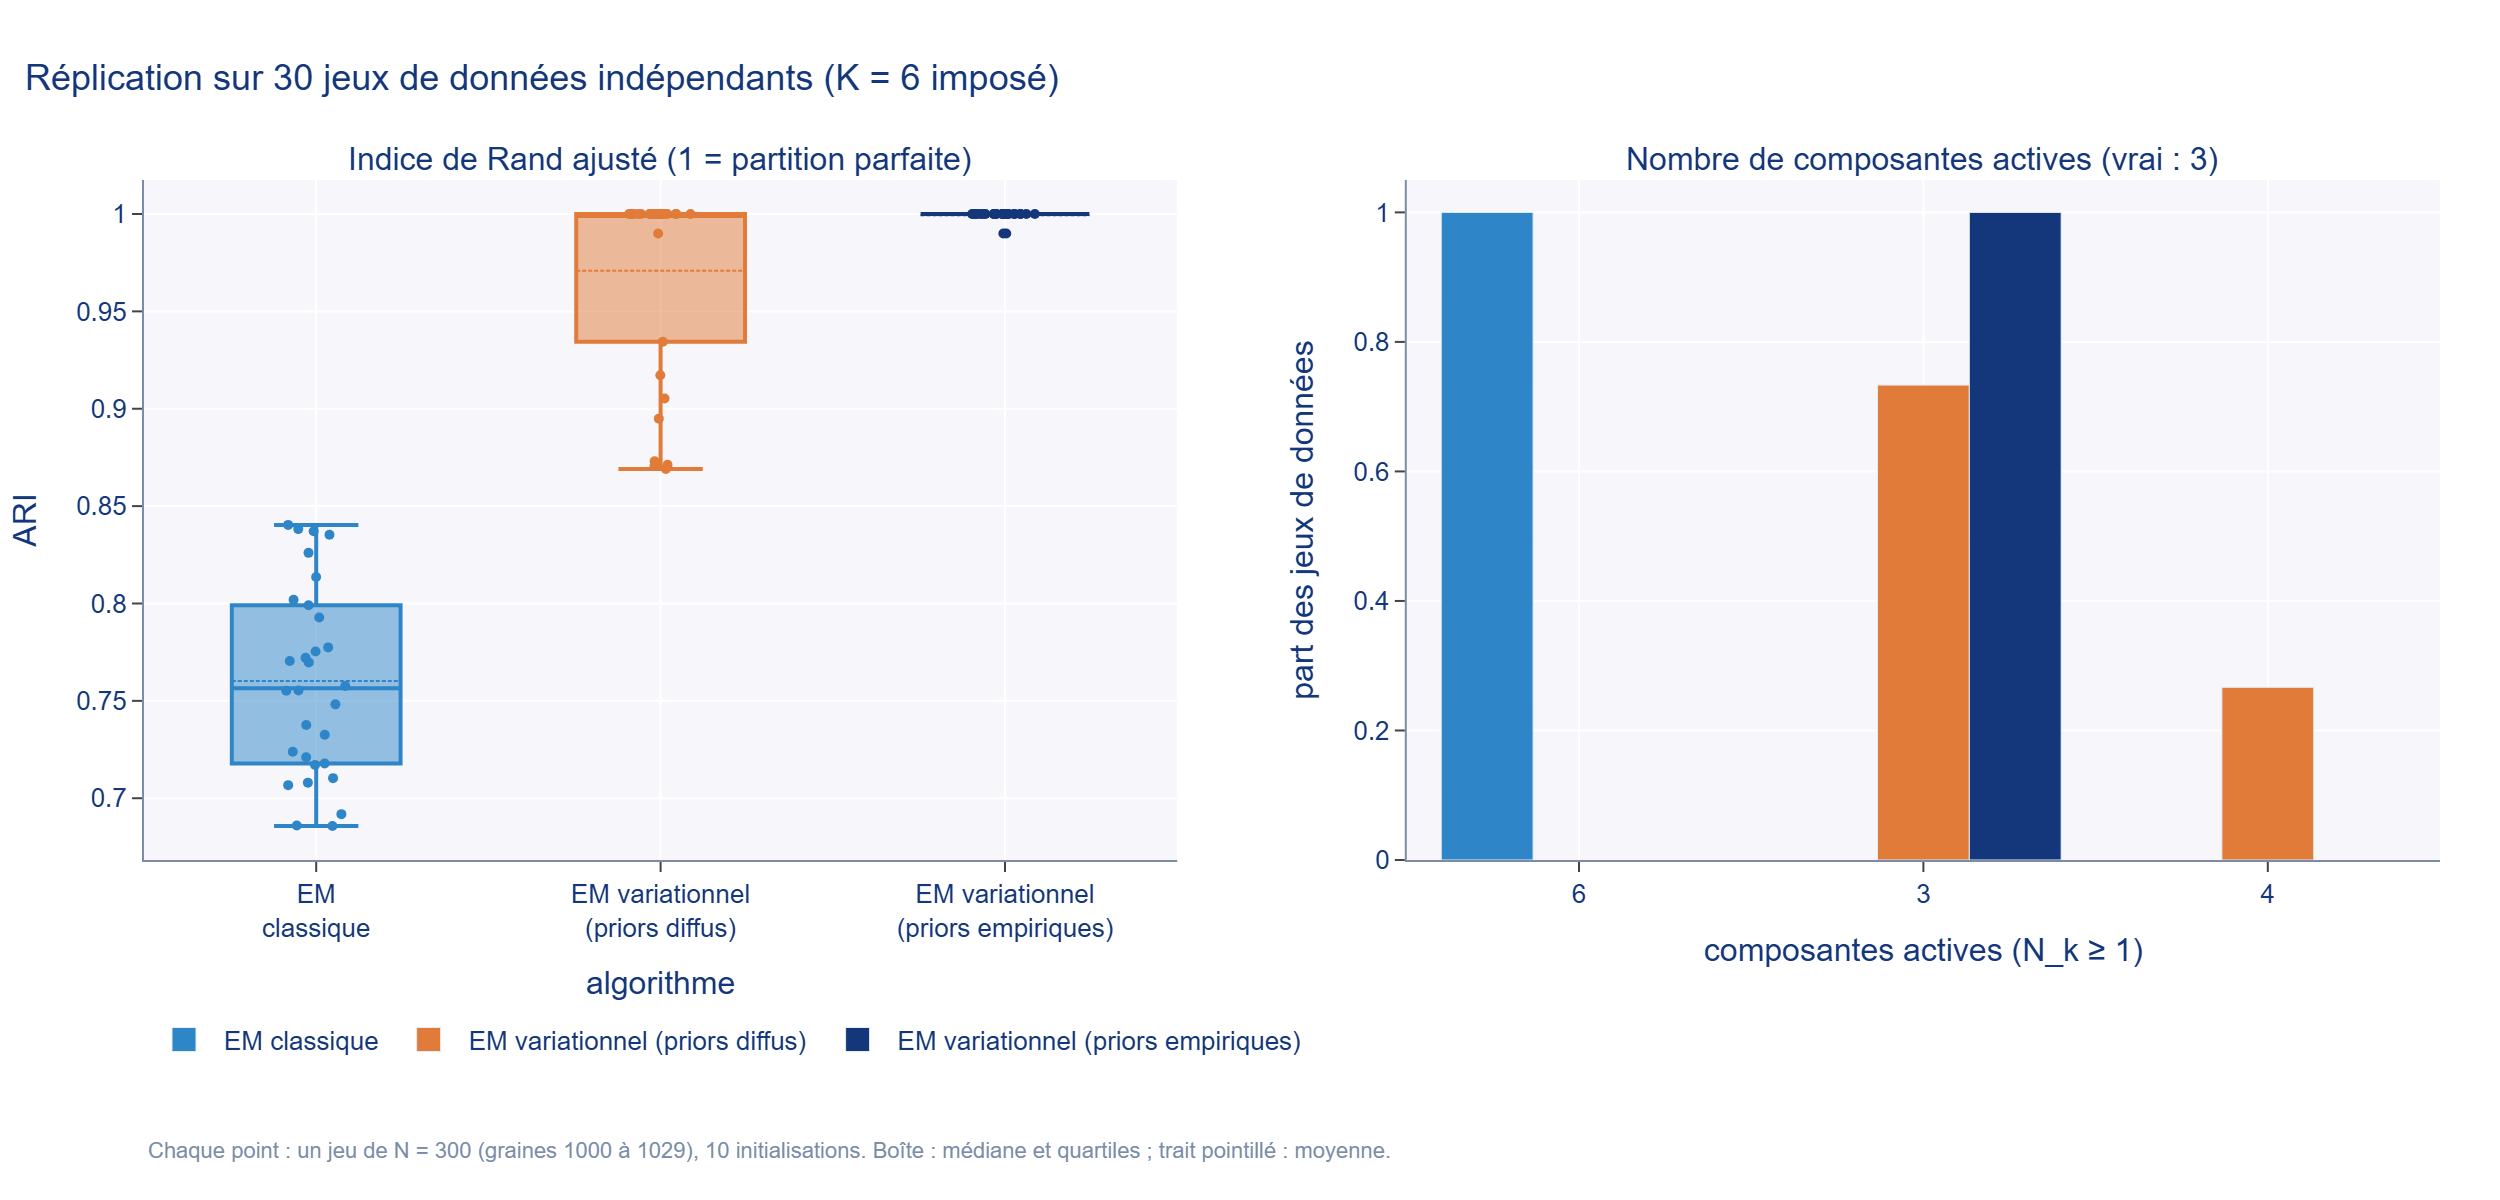
\includegraphics[width=0.95\textwidth]{figures/fig12.png}
\caption{Distribution de l'indice de Rand ajusté (à gauche, un point par jeu de données) et du nombre de composantes actives (à droite) sur 30 jeux de données indépendants.}
\label{fig:2_11}
\end{figure}
H1 est soutenue pour les deux jeux de priors (intervalle bootstrap strictement positif, tableau~\ref{tab:2_16}). H2 est soutenue pour les deux jeux, avec des marges très différentes (tableau~\ref{tab:2_15}) : plus nette avec les priors empiriques qu'avec les priors diffus. H3 est confirmée : le résultat dépend des priors. \par\medskip\noindent\textbf{Portée de ces hypothèses. }H1 et H2 sont quasi tautologiques et ne testent pas la thèse de ce mémoire : H2 compare le VB à un EM dont $K=6$ est imposé, qui ne peut pas retrouver trois composantes par construction ; H1 porte sur 30 différences de même signe, pour lesquelles un intervalle bootstrap n'apporte rien. Les 30 jeux proviennent en outre d'un seul générateur (trois gaussiennes isotropes séparées) : c'est une réplication statistique, non une réplication sur des schémas de génération différents. Les priors diffus sont ceux qu'on utiliserait sans connaissance préalable, et le résultat des priors empiriques n'est pas une propriété du VB seul. Les hypothèses informatives sont celles des sections 2.3.14 à 2.3.19, qui comparent le VB à EM-BIC, EM-ICL et MAP-EM sur plusieurs générateurs, avec test apparié et marge d'équivalence.

\subsection{Grille de $\alpha_0$ autour du seuil $d/2$ (scénario S8)}
La grille du tableau 2.8 (0,001 à 10) saute la zone de transition. La grille $\alpha_0 \in \{1;\,1{,}5;\,2;\,2{,}5;\,3;\,5;\,10\}$ est donc évaluée pour les trois types de covariance, dont les seuils théoriques de Rousseau et Mengersen (2011) sont $d/2 = 2{,}5$ (pleine), $2$ (diagonale) et $1{,}5$ (sphérique) en dimension 2. L'hypothèse testée est que le nombre de composantes actives change de régime autour de ces seuils ; la théorie portant sur le posterior exact, l'observation d'un seuil ailleurs n'est pas une réfutation de la théorie mais une propriété du champ moyen. Résultats : tableau~\ref{tab:S8}. Le tableau indique la part d'exécutions non convergées, et pour les covariances non pleines le critère est une approximation (section 3.2.2).

\tableauGenere{S8_alpha0}

\textbf{Lecture. }En covariance pleine, le nombre de composantes actives reste voisin de 3 jusqu'à $\alpha_0 = 2{,}5$, croît légèrement à $\alpha_0 = 3$ puis atteint $K_{\max}=6$ à $\alpha_0 = 5$ : le basculement se situe entre 3 et 5, un peu au-delà du seuil théorique $d/2 = 2{,}5$. En covariance diagonale et sphérique, le nombre de composantes actives augmente plus tôt et plus progressivement, et l'ordre des transitions (pleine, diagonale, sphérique) est celui que prédisent les seuils $d/2$ décroissants, sans que les valeurs précises $2{,}5$, $2$ et $1{,}5$ soient observées nettement : le critère de ces deux dernières est une approximation, et le comportement est celui d'une transition lisse, non d'un seuil net. Ce résultat \emph{ne confirme ni ne réfute} la théorie de Rousseau et Mengersen (2011), qui porte sur le posterior exact : il montre que le champ moyen présente une transition de même ordre, située dans la même zone, et que $\alpha_0$ pilote $\hat K$ dans cette zone.

\subsection{Couverture des intervalles de crédibilité (hypothèse H6)}
La sous-estimation de variance du champ moyen (section 1.5.4) ne peut être jugée que par la couverture empirique des intervalles à 90 \% sur des jeux dont les paramètres vrais sont connus. Cette mesure est faite sur le jeu semi-synthétique du cas climatique (section 3.1.1), pour le VB et pour le bootstrap de l'EM ; la couverture empirique est rapportée avec son intervalle de Wilson au tableau~\ref{tab:climat_couverture}. Les intervalles de crédibilité et de confiance ne mesurent pas le même objet : leur couverture sur la valeur vraie est une comparaison de calibration, non de justesse bayésienne.

\tableauGenere{climat_couverture}

\textbf{Lecture. }Les intervalles de crédibilité à 90 \% du VB sur les poids $\pi_k$ ont une couverture empirique dont l'intervalle de Wilson est inférieur à la valeur nominale (sous-couverture), alors que leur couverture sur les moyennes des composantes est compatible avec 90 \% ; le bootstrap de l'EM est proche du nominal pour les moyennes et au moins nominal pour les poids. La sous-estimation de variance du champ moyen (section 1.5.4) est donc observée sur les poids, pas sur les moyennes, dans ce jeu semi-synthétique, pour les paramètres des composantes appariées au modèle vrai et les jeux où le VB retrouve cinq composantes ($N \geq 120$). Cette mesure ne vaut pas pour d'autres modèles ni pour d'autres priors.

\subsection{Baseline EM-BIC, chevauchement, déséquilibre et sous-estimation de $K$ (S1 à S3)}
Chaque scénario compte au moins 30 réplications et compare, par test apparié, EM-$K$, EM-$K_{\max}$, EM-BIC, EM-ICL, MAP-EM et le VB (priors empiriques et diffus), avec le critère d'arrêt de la figure~\ref{fig:boucle_arret} (protocole de la figure~\ref{fig:protocole}). S1 fait varier la séparation de 1 à 5 écarts-types ; S2 fixe des poids de 80, 15 et 5 \% ; S3 impose un $K$ choisi (3) inférieur au $K$ vrai (4 à 6), ce qui borne aussi le $K_{\max}$ du VB. Les équivalences sont jugées par TOST avec une marge de 0,03 en ARI ; la correction de Holm est appliquée sur l'ensemble des tests de la grille.

\begin{figure}[H]
\centering
\begin{tikzpicture}[>=Stealth,
    b/.style={draw=navy,rounded corners=2pt,align=center,font=\scriptsize,fill=ciel!20,minimum height=0.8cm,text width=2.5cm},
    g/.style={draw=bleu,rounded corners=2pt,align=center,font=\scriptsize,fill=bleu!15,minimum height=0.55cm,text width=3.4cm}]
  \node[b] (don) at (0,0) {données (au moins 30 réplications, graines fixées)};
  \node[g] (a1) at (4.2,1.95) {EM-$K$ ($K$ connu)};
  \node[g] (a2) at (4.2,1.3)  {EM-$K_{\max}$};
  \node[g] (a3) at (4.2,0.65) {EM-BIC};
  \node[g] (a4) at (4.2,0)    {EM-ICL};
  \node[g] (a5) at (4.2,-0.65) {MAP-EM};
  \node[g] (a6) at (4.2,-1.3) {VB, priors empiriques};
  \node[g] (a7) at (4.2,-1.95) {VB, priors diffus};
  \node[b] (mes) at (7.9,0) {mesures : $\hat K$, ARI, log-vraisemblance hors échantillon, dégénérescence, temps};
  \node[b] (tst) at (11.5,0) {tests appariés, TOST, Wilcoxon, correction de Holm};
  \draw[->] (don) -- (a1.west);
  \draw[->] (don) -- (a4.west);
  \draw[->] (don) -- (a7.west);
  \draw[->] (a1.east) -- (mes.west);
  \draw[->] (a4.east) -- (mes.west);
  \draw[->] (a7.east) -- (mes.west);
  \draw[->] (mes) -- (tst);
  \node[font=\scriptsize,text=navy] at (5.9,-2.7) {même critère d'arrêt (figure~\ref{fig:boucle_arret}) pour tous les bras};
\end{tikzpicture}
\caption{Protocole « 5 EM + VB » : tous les bras partagent le critère d'arrêt, les graines et les mesures ; chaque comparaison est appariée par réplication.}
\label{fig:protocole}
\end{figure}

\begin{figure}[H]
\centering
\begin{tikzpicture}[>=Stealth,
    boite/.style={draw=navy,rounded corners=2pt,minimum height=0.9cm,align=center,font=\footnotesize,fill=ciel!20,text width=3.0cm},
    test/.style={draw=bleu,rounded corners=2pt,align=center,font=\footnotesize,fill=bleu!12,text width=3.6cm,minimum height=1.1cm}]
  \node[boite] (init) at (0,0) {initialisation\\$\theta_0$ ou $q_0$, $n_M=0$};
  \node[boite] (E) at (4.2,0) {étape E\\$r_{ik}$ et critère $c_t$};
  \node[test] (T) at (8.8,0) {$\lvert c_t-c_{t-1}\rvert\le \mathrm{tol}\cdot\max(\lvert c_{t-1}\rvert,1)$ ?};
  \node[boite,fill=navy!15] (S) at (13.0,0) {arrêt\\\texttt{converge}=vrai};
  \node[test] (P) at (8.8,-2.2) {$n_M=500$ ?\\sinon étape M};
  \node[boite,fill=navy!15] (S2) at (13.0,-2.2) {arrêt\\\texttt{converge}=faux};
  \node[boite] (M) at (4.2,-2.2) {étape M\\$n_M\leftarrow n_M+1$};
  \draw[->] (init) -- (E);
  \draw[->] (E) -- (T);
  \draw[->] (T) -- node[above,font=\scriptsize]{oui} (S);
  \draw[->] (T) -- node[right,font=\scriptsize]{non} (P);
  \draw[->] (P) -- node[above,font=\scriptsize]{oui} (S2);
  \draw[->] (P) -- node[above,font=\scriptsize]{non} (M);
  \draw[->] (M) -- (E);
\end{tikzpicture}
\caption{Critère d'arrêt commun à l'EM, au MAP-EM, à l'EM variationnel et au pLSA. Le critère $c$ est la log-vraisemblance totale (EM) ou l'ELBO total (VB, covariance pleine), évalué après chaque étape E et avant l'étape M. Tolérance relative $10^{-6}$ et plafond commun de 500 étapes M ; $n_M$ est le nombre d'itérations rapporté.}
\label{fig:boucle_arret}
\end{figure}


\tableauGenere{S1_chevauchement}
\tableauGenere{S2_desequilibre}
\tableauGenere{S3_sous_estimation}

\textbf{Lecture (S1 à S3). }Les différences appariées d'ARI entre le VB à priors empiriques et EM-BIC sont décidées par le tableau~\ref{tab:grille_scenarios} (équivalence à $\pm0{,}03$ ou test des rangs de Wilcoxon, correction de Holm). (i) \emph{Chevauchement.} Lorsque les groupes sont séparés de 4 à 5 écarts-types, les deux méthodes sont équivalentes. À 1 écart-type, aucune ne retrouve la structure ($\hat K$ proche de 1, ARI proche de 0 pour les deux). Aux séparations intermédiaires (2 et 3 écarts-types), le VB à priors empiriques obtient un ARI supérieur à celui de EM-BIC, dont le $\hat K$ moyen reste trop bas ; EM-ICL, plus pénalisant, sélectionne souvent un seul groupe. (ii) \emph{Déséquilibre 80/15/5.} L'écart $\lvert\hat K - K\rvert$ du VB à priors empiriques et de EM-BIC est équivalent (marge de 0,5 composante, tableau~\ref{tab:grille_scenarios}). EM-BIC et EM-ICL perdent parfois la composante à 5 \% ($\hat K$ moyen inférieur à 3), alors que le VB tend à conserver au moins trois composantes ; l'ARI du VB est néanmoins un peu inférieur à celui d'EM-BIC et d'EM-ICL, résultat défavorable au VB qui est conservé. (iii) \emph{Sous-estimation de $K$.} Avec $K$ choisi égal à 3 pour des mélanges de 4 à 6 groupes, l'EM à $K=3$ et le VB à $K_{\max}=3$ ne peuvent pas corriger l'erreur de spécification ; l'ARI du VB à $K_{\max}=K$ est toutefois supérieur à celui de l'EM à $K$ fixé, l'écart étant compatible avec la régularisation par les priors. En revanche, le VB à $K_{\max}=10$ avec priors diffus retrouve un $\hat K$ proche de $K$ vrai et l'ARI le plus élevé du scénario, alors que le VB à $K_{\max}=10$ avec priors empiriques sous-estime $K$ comme EM-ICL. \textbf{Cela confirme la thèse du mémoire :} le résultat du VB dépend du jeu de priors, c'est-à-dire que la sélection de $K$ est déplacée vers le choix des hyperparamètres, et non supprimée. Ces comparaisons utilisent des priors empiriques pour le VB (Bayes empirique, double usage des données) ; elles ne démontrent donc pas la supériorité de l'inférence variationnelle.

\subsection{Queues épaisses, dimension croissante et petit effectif (S4 à S6)}
S4 génère des composantes de Student à 3 degrés de liberté ; S5 fait varier $D$ dans $\{2, 5, 10, 20\}$ ; S6 fait varier $N$ de 30 à 1\,000 et rapporte le taux d'ajustements dégénérés (valeur propre minimale de $\Sigma_k$ inférieure à $10^{-6}$ fois sa trace, ou $N_k < D+1$) pour chaque algorithme. Comme le code de l'EM ajoute $\varepsilon I$ avec $\varepsilon = 10^{-6}$ (section 3.2.1), le taux mesuré est celui de l'EM régularisé.

\tableauGenere{S4_queues_epaisses}
\tableauGenere{S5_dimension}
\tableauGenere{S6_petit_N}

\textbf{Lecture (S4 à S6). }(S4, queues épaisses.) Les composantes de Student dégradent la sélection de $K$ pour toutes les méthodes (le $\hat K$ moyen dépasse 3) ; le VB à priors empiriques obtient un ARI supérieur à EM-BIC (tableau~\ref{tab:grille_scenarios}), au prix de taux de dégénérescence non négligeables pour la plupart des bras. (S5, dimension.) À $D=2$ les deux méthodes sont équivalentes. À $D=5$, EM-BIC a un ARI supérieur à celui du VB à priors empiriques : \emph{c'est un résultat défavorable au VB}, conservé tel quel. À $D=10$ aucune des méthodes ne retrouve $K=3$ avec $N=300$ et la différence est indéterminée. À $D=20$, EM-BIC sélectionne un seul groupe (ARI nul) tandis que le VB, dont les composantes restent actives, obtient un ARI de l'ordre de 0,5 : cet écart tient à l'échec de la sélection par BIC en grande dimension à $N$ fixé, non à une qualité de l'inférence variationnelle ; les bras à $K$ élevé ont des taux de dégénérescence proches de 1 à $D \geq 10$. (S6, petit effectif.) Pour $N \leq 120$, le VB à priors empiriques produit significativement moins d'ajustements dégénérés que l'EM à $K_{\max}$ imposé (tableau~\ref{tab:grille_scenarios}) ; à $N=300$ la différence est à la limite de la significativité après correction de Holm ; à $N=1\,000$ les taux sont équivalents (nuls). Cette comparaison est celle de la \emph{même} capacité $K_{\max}=10$ : l'EM à $K=10$ sur 30 points est mal posé par construction, et la baseline EM-BIC choisit un $K$ proche de 10 à $N=30$ et est elle aussi dégénérée à cet effectif, puis évite la plupart des dégénérescences dès $N=60$ en retenant un $K$ plus petit. Les taux sont ceux de l'EM \emph{régularisé} par $\varepsilon I$ (section 3.2.1) ; ils ne disent rien de l'EM non régularisé.

\subsection{Aberrations : proportion et amplitude variées (S7)}
Le scénario S7 remplace l'unique tirage de la section 2.3.12 par 30 tirages ou plus pour chaque couple (proportion, amplitude), avec la baseline EM-BIC.

\tableauGenere{S7_aberrations}

\textbf{Lecture (S7). }Sur 30 tirages pour chaque couple (proportion, amplitude), le VB à priors empiriques et EM-BIC sont équivalents en ARI (marge $\pm0{,}03$) dans tous les cas testés (tableau~\ref{tab:grille_scenarios}). Les aberrations ne séparent donc pas les deux méthodes en ARI : l'interprétation de la section 2.3.12 (« absorption dans une composante diffuse ») et l'idée d'un avantage de robustesse du VB ne sont \emph{pas} soutenues par ce scénario. Elles se manifestent plutôt sur le $\hat K$ : EM-BIC ajoute des composantes pour les aberrations de forte amplitude ($\hat K$ élevé), le VB à priors empiriques en ajoute moins, sans effet sur l'ARI. Aucune composante uniforme de fond n'a été comparée (non testé).

\tableauGenere{grille_scenarios}

\subsection{Plan factoriel sur les priors et seuil d'activité (S9 et S10)}
Le plan factoriel fait varier $\alpha_0$, $\beta_0$, $\nu_0$ et l'échelle de $W_0$ ; la part de variance du nombre de composantes actives expliquée par chaque facteur est rapportée (tableau~\ref{tab:S9}). Le scénario S10 montre la sensibilité du nombre de composantes actives au seuil (0,5 \%, 1 \%, 5 \% de $N$, et $N_k \geq 1$) : tant que ce nombre dépend du seuil, il ne constitue pas une mesure fiable de $\hat K$.

\tableauGenere{S9_decomposition_variance}
\tableauGenere{S10_seuil_activite}

\textbf{Lecture (S9 et S10). }Le plan factoriel attribue à la concentration $\alpha_0$ la plus grande part de la variance du nombre de composantes actives, devant $\beta_0$, l'échelle de $W_0$ et $\nu_0$ (tableau~\ref{tab:S9}) ; le résidu (interactions) reste substantiel. La sélection de $K$ par le VB est donc surtout pilotée par $\alpha_0$, ce qui est une dépendance aux hyperparamètres au sens de la thèse. Le seuil d'activité a peu d'effet dans ce jeu (tableau~\ref{tab:S10}) : les trois valeurs relatives (0,5, 1 et 5 \% de $N$) et $N_k \geq 1$ donnent des nombres de composantes actifs très voisins, sauf pour $\alpha_0 = 2{,}5$ où le seuil à 5 \% en retire quelques-unes. Le caractère arbitraire de $N_k \geq 1$ souligné à la section 2.3.4 est donc réel mais de portée limitée sur cette distribution de poids, qui est nettement bimodale (composantes soit écrasées, soit de poids proche d'un tiers).

\subsection{Coût de la sélection de $K$ en temps total}
\tableauGenere{cout_selection}

Le rapport des temps médians entre le pipeline EM-BIC complet ($K$ de 1 à 10, dix initialisations) et un ajustement VB à dix initialisations est supérieur à 1 pour tous les effectifs du tableau~\ref{tab:cout_selection} (intervalle bootstrap strictement au-dessus de 1, hypothèse H4) : le pipeline EM-BIC coûte plus qu'un VB, de façon croissante avec $N$ au début de la plage. Ce résultat s'oppose à la lecture « le VB est plus coûteux » tirée du coût par itération et confirme que la comparaison pertinente se fait en temps total jusqu'au modèle final. Il reste propre à une machine (et à une implémentation PyTorch sans parallélisation fine) et à une baseline à balayage complet et dix initialisations.

\subsection{Métriques sans étiquette}
L'ARI suppose une vérité terrain et dépend du nombre de composantes. La silhouette n'est comparable qu'à $K$ égal. Le tableau des scénarios rapporte donc aussi la log-vraisemblance moyenne hors échantillon (plug-in pour tous les bras ; prédictive de Student en plus pour le VB, afin d'isoler l'effet de la loi prédictive) et le taux d'ajustements dégénérés.


\section{Analyse des résultats et synthèse}
L'étude conduite dans ce chapitre ne désigne pas un meilleur algorithme : elle décrit des déplacements. Le VB transfère la sélection de $K$ vers le choix de $K_{\max}$, des hyperparamètres et du seuil d'activité ; il fournit une incertitude approchée dont la couverture est mesurée ; il coûte plus par ajustement que l'EM, ce qui n'établit pas un coût plus élevé que le pipeline EM-BIC en temps total. Lorsque $K$ est correctement spécifié, les deux algorithmes sont de qualité comparable (à confirmer par équivalence, tableaux des scénarios S1 à S3). La comparaison à $K = 6$ imposé est défavorable à l'EM par construction et ne sert que d'illustration du mécanisme d'élagage.

Le tableau~\ref{tab:2_17} remplace les anciennes listes d'avantages et d'inconvénients par une grille « axe $\times$ preuve » : chaque ligne renvoie à une expérience, à un théorème, ou porte la mention « non testé ».

\tableauGenere{grille_axe_preuve}
Cette synthèse met en évidence que le choix entre les deux algorithmes ne doit pas être envisagé comme un choix entre une méthode « meilleure » et une méthode « moins bonne » dans l'absolu, mais comme un arbitrage dépendant du contexte applicatif  arbitrage que le chapitre 3 explore plus en détail à travers plusieurs domaines d'application concrets. Aucune ligne de la grille n'autorise à parler de supériorité.

\section{Discussion critique du protocole expérimental}
Par honnêteté scientifique, il convient de discuter explicitement les limites du protocole expérimental suivi dans ce chapitre, avant d'en tirer des conclusions générales. Premièrement, la majorité des expériences (sections 2.3.1 à 2.3.10 et 2.3.12) reposent sur un unique jeu de données synthétique, construit par assemblage de trois gaussiennes isotropes bien séparées. Ce choix méthodologique, motivé par la volonté de disposer d'une vérité terrain non ambiguë pour calculer l'indice de Rand ajusté, favorise par construction le scénario le plus propice à l'EM variationnel : des groupes qui sont effectivement des gaussiennes, bien séparées, et de tailles comparables. La section 2.3.11, en introduisant le jeu de données réel Iris, a précisément eu pour objet de vérifier dans quelle mesure les conclusions tirées du cas synthétique se généralisent à un contexte moins favorable, et a montré que ce n'est pas systématiquement le cas : lorsque les groupes réels se chevauchent ou s'écartent de la forme gaussienne, l'avantage de l'EM variationnel peut s'atténuer, voire s'inverser localement.

Deuxièmement, les expériences des sections 2.3.1 à 2.3.12 reposent sur une seule graine de génération des données (graine 42). La section 2.3.13 lève en partie cette limite en répétant le protocole de la section 2.3.1 sur trente jeux indépendants, avec intervalles de confiance ; les autres expériences (Iris, valeurs aberrantes, type de covariance, scalabilité) n'ont pas été répliquées de cette manière, et la mesure des temps de calcul reste propre à une machine et à une implémentation.

Troisièmement, les dimensions considérées dans ce chapitre restent modestes (D = 2 pour la majorité des expériences, D = 4 pour Iris, D allant jusqu'à 20 pour l'étude de scalabilité de la section 2.3.6). Les grandes dimensions, fréquentes dans les applications réelles évoquées au chapitre 3 (bio-informatique, traitement d'image), posent des défis supplémentaires  malédiction de la dimensionnalité, estimation de matrices de covariance de grande taille à partir d'un nombre limité d'observations  qui n'ont pas été explorés empiriquement ici, au-delà des mesures de temps de calcul de la section 2.3.6. Ces trois limites, prises ensemble, invitent à interpréter les résultats de ce chapitre comme une démonstration rigoureuse et reproductible du mécanisme théorique décrit au chapitre 1, plutôt que comme une garantie de supériorité universelle de l'EM variationnel sur l'EM classique dans toutes les configurations de données possibles  nuance que le guide de décision pratique proposé à la section 3.5 s'efforce de refléter fidèlement.

Une quatrième limite, de nature plus méthodologique, mérite également d'être signalée : l'ensemble des métriques externes utilisées dans ce chapitre (ARI, score de silhouette) supposent implicitement l'existence d'une partition de référence contre laquelle comparer les résultats des algorithmes, ce qui n'est vrai que pour les données synthétiques et pour Iris, dont les étiquettes d'espèces sont connues indépendamment des variables mesurées. Dans la grande majorité des applications réelles évoquées au chapitre 3, en particulier en bio-informatique et en traitement du langage naturel, une telle vérité terrain n'existe tout simplement pas  la détermination du nombre « correct » de sous-populations cellulaires ou de thématiques textuelles étant précisément l'objet de l'analyse plutôt qu'une donnée préalable. Dans ces contextes d'analyse non supervisée pure, l'évaluation de la qualité d'un modèle de mélange doit nécessairement s'appuyer sur des critères internes  l'ELBO lui-même pour l'EM variationnel (section 1.7.6), ou les critères BIC/AIC pour l'EM classique (section 2.2.3) , dont ce chapitre a montré, à la section 2.3.3, qu'ils ne sont pas directement comparables en échelle absolue entre les deux algorithmes, ce qui limite d'autant la possibilité de trancher objectivement, en l'absence de vérité terrain, lequel des deux modèles offre le meilleur ajustement aux données.

Une cinquième série de limites n'était pas reconnue dans la première version de ce chapitre et conditionne la lecture des sections 2.3.2 à 2.3.13 : (i) la baseline EM-BIC/ICL et le MAP-EM manquaient ; (ii) les critères d'arrêt de l'EM et du VB n'étaient pas comparables, ce qui affectait les nombres d'itérations et les temps (désormais harmonisés, section 2.3.1) ; (iii) le seuil $N_k \geq 1$ pour déclarer une composante active est arbitraire, et le nombre de composantes actives n'est pas une mesure fiable (S10) ; (iv) l'ARI à $K = 6$ est un artefact de la fragmentation des composantes excédentaires ; (v) les expériences sur les aberrations reposaient sur un seul tirage ; (vi) les singularités n'étaient pas comptées, et l'EM utilise une régularisation $\varepsilon I$ ; (vii) le seuil théorique $d/2$ de $\alpha_0$ n'avait pas été confronté à une grille adaptée.


%% ==== PARTIE 3 ====
\part{APPLICATIONS ET IMPLÉMENTATION}

%% ==== CHAPITRE : APPLICATIONS ET IMPLÉMENTATION ====
\chapter{APPLICATIONS ET IMPLÉMENTATION}
Les deux chapitres précédents ont établi les fondements théoriques de l'EM classique et de l'EM variationnel, puis confronté ces deux algorithmes sur un cas d'étude synthétique. Ce troisième et dernier chapitre s'attache à replacer ces algorithmes dans leur contexte applicatif réel, en explorant plusieurs domaines dans lesquels ils sont couramment employés, avant de présenter une implémentation complète en langage Python, accompagnée d'une analyse détaillée des résultats expérimentaux obtenus.

\section{Applications pratiques}
Ce chapitre distingue trois statuts de preuve. Le \emph{cas principal} (régimes climatiques du Cameroun) est conçu pour tester ensemble les avantages et les inconvénients du sujet sur des données réelles à structure chevauchante, déséquilibrée et non gaussienne. Le \emph{cas secondaire} (rendements du S\&P 500) évalue la gestion du risque avec des données réelles mais une période de test marquée par un changement de régime. Une \emph{comparaison pLSA contre LDA} sur corpus réel traite le cadre des modèles de thèmes. Les autres domaines (vision, bio-informatique, recommandation) sont présentés en \emph{revue de la littérature} : aucune expérience n'y est conduite, et les affirmations qui n'ont ni source ni test sont signalées comme « non testé ».

Le fil conducteur est la thèse de ce mémoire : le VB ne « bat » pas l'EM ; il déplace la sélection de $K$ vers le choix des hyperparamètres, apporte une incertitude approchée, au prix d'un coût et d'une sensibilité aux priors. Le choix entre les deux dépend des contraintes opérationnelles (temps de calcul, confiance dans $K$, besoin d'une incertitude en aval, robustesse requise), et chaque lien entre une contrainte et un algorithme doit être soutenu par la grille du tableau~\ref{tab:2_17}.

\subsection{Cas principal : régimes climatiques du Cameroun}
\textbf{Question. }Le Cameroun est officiellement découpé en cinq zones agro-écologiques (soudano-sahélienne, hautes savanes guinéennes, hauts plateaux de l'Ouest, forêt à pluviométrie monomodale, forêt à pluviométrie bimodale). À partir de variables climatiques et d'altitude seulement, sans connaître $K$, (i) l'EM classique, avec $K$ choisi par BIC ou ICL, et l'EM variationnel avec élagage retrouvent-ils une structure cohérente avec un zonage ? (ii) Dans quelles conditions (effectif, dimension, chevauchement, déséquilibre, besoin d'incertitude, budget de calcul) l'un est-il préférable ? (iii) Les intervalles de crédibilité du VB sont-ils fiables (couverture) ou trop étroits ? Ce cas teste ensemble les avantages et les inconvénients du sujet sur des données réelles à structure chevauchante, déséquilibrée et non gaussienne.

\textbf{Données. }Climat : WorldClim 2.1 (climatologies 1970-2000, résolution de 2,5 minutes d'arc, soit environ 4,6 km), archives GeoTIFF \texttt{wc2.1\_2.5m\_bio.zip} et \texttt{wc2.1\_2.5m\_elev.zip} (Fick et Hijmans, 2017). La licence autorise l'usage académique et non commercial et \emph{interdit la redistribution sans autorisation} : les fichiers ne sont pas versionnés avec le code, que le script \texttt{cas\_pratique\_climat.py --preparer} télécharge, en journalisant la date et l'empreinte SHA-256 des archives. Variables ($D=5$) : température moyenne annuelle (bio1), saisonnalité de la température (bio4), précipitations annuelles en logarithme (bio12), saisonnalité des précipitations (bio15), altitude ; extension à $D=20$ (toutes les variables bioclimatiques et l'altitude). Les données sont standardisées et identiques pour tous les algorithmes.

\textbf{Références. }(a) Les zones agro-écologiques officielles ($K_{\text{réf}}=5$) : aucun shapefile téléchargeable n'a été trouvé (une carte de l'IRAD, 2005, n'est publiée qu'en figure) ; le script accepte un fichier fourni par l'utilisateur (option \texttt{--zones}) et, \emph{à défaut, la référence est Köppen--Geiger seul}, ce que les tableaux indiquent. (b) Köppen--Geiger (Beck et al., 2018), carte à 1 km, dont la licence doit être confirmée sur la page de distribution avant tout dépôt. Les étiquettes sont elles-mêmes définies à partir du climat : l'ARI mesure la cohérence avec un zonage, non une vérité ; c'est pourquoi la log-vraisemblance hors bloc, sans étiquette, est rapportée.

\textbf{Bras. }EM-5 ($K$ connu), EM-10 ($K$ trop grand), EM-BIC et EM-ICL ($K$ de 1 à 10), MAP-EM (mêmes priors que le VB, $K=10$), VB à priors empiriques et à priors diffus ($K_{\max}=10$, $\alpha_0 = 1/K_{\max}$), et une grille de VB sur $(\alpha_0, \beta_0, \nu_0, W_0)$. Mêmes critère d'arrêt (figure~\ref{fig:boucle_arret}), 10 initialisations par ajustement, covariance pleine, graines fixées. Une composante est active si $N_k/N \geq 1\,\%$ (sensibilité aux seuils de 0,5, 1 et 5 \%, et $N_k \geq 1$).

\textbf{Plan d'échantillonnage. }Les cellules voisines sont corrélées : pour $N \in \{30, 60, 120, 500, 2\,000\}$ et le jeu complet, 100 sous-échantillons espacés d'une distance minimale sont tirés, et l'évaluation hors échantillon se fait par blocs d'environ 100 km (figure~\ref{fig:echant_spatial}). Un jeu semi-synthétique complète le dispositif : un modèle à $K=5$ est ajusté à $N$ complet, puis 200 jeux de taille $N$ sont simulés à partir de lui, de sorte que la vérité (paramètres, chevauchement, déséquilibre) est connue et réaliste.

\begin{figure}[H]
\centering
\begin{tikzpicture}[scale=0.9]
  \foreach \i in {0,...,5} {\foreach \j in {0,...,3} {\draw[gray!50] (\i*1.5,\j*1.5) rectangle ++(1.5,1.5);}}
  \fill[bleu!30,opacity=0.5] (4.5,1.5) rectangle (6,3);
  \fill[bleu!30,opacity=0.5] (1.5,3) rectangle (3,4.5);
  \foreach \p in {(0.4,0.5),(2.3,0.9),(4.6,0.4),(7.0,1.1),(1.0,2.6),(3.4,2.2),(7.0,2.8),(8.0,2.3),(0.7,4.9),(3.9,4.0),(6.3,4.6),(8.5,5.1)}
    \fill[navy] \p circle (2.2pt);
  \node[font=\scriptsize,text=bleu] at (5.25,3.3) {bloc de test};
  \draw[<->,navy] (0.4,-0.35) -- node[below,font=\scriptsize]{$d_{\min}$} (2.3,-0.35);
\end{tikzpicture}
\caption{Échantillonnage spatial : les points d'apprentissage (noirs) sont espacés d'au moins $d_{\min}$ ; l'évaluation se fait sur des blocs d'environ 100 km sans point d'apprentissage (validation croisée par blocs). Schéma illustratif.}
\label{fig:echant_spatial}
\end{figure}


\textbf{Hypothèses, fixées avant les résultats. }Chacune peut être rejetée dans un sens ou dans l'autre, l'équivalence est une issue légitime, et la correction de Holm est appliquée sur l'ensemble des tests.

\begin{table}[H]
\centering
\small
\setlength{\tabcolsep}{0.1cm}
\begin{tabular}{|p{0.9cm}|p{2.6cm}|p{5.4cm}|p{5.6cm}|}
\hline
\textbf{N°} & \textbf{Axe} & \textbf{Hypothèse} & \textbf{Critère de décision} \\
\hline
H1 & Sélection de $K$ & VB et EM-BIC/ICL ne diffèrent pas de plus de 0,5 composante de $K_{\text{réf}}=5$ (semi-synthétique) & IC bootstrap à 95 \% de la différence de $\lvert\hat K - K_{\text{réf}}\rvert$ dans $[-0{,}5;\,0{,}5]$, Wilcoxon apparié \\
\hline
H2 & Qualité à $N$ complet & ARI et log-vraisemblance hors bloc équivalents (marges $\pm0{,}03$ en ARI, $\pm0{,}02$ nat par observation) & TOST, IC par blocs spatiaux \\
\hline
H3 & Petit $N$ & VB : moins d'ajustements dégénérés que EM-10 pour $N \leq 120$ & Test exact de Fisher, par $N$ \\
\hline
H4 & Coût & Le pipeline EM-BIC (K de 1 à 10, 10 initialisations) coûte plus qu'un VB à 10 initialisations & Rapport des temps médians avec IC ; décision si le ratio est supérieur à 1 \\
\hline
H5 & Hyperparamètres & La variance de $\hat K$ du VB due aux priors est au moins égale à celle de l'EM due à l'initialisation & Décomposition de variance sur le plan factoriel \\
\hline
H6 & Incertitude & Couverture des intervalles de crédibilité à 90 \% du VB inférieure à 90 \% ; le bootstrap de l'EM est plus proche du nominal & Couverture empirique, IC de Wilson, 200 jeux semi-synthétiques \\
\hline
H7 & Chevauchement & Le VB fusionne plus de zones voisines que EM-BIC & Matrice de confusion, nombre de zones fusionnées, ARI par zone \\
\hline
H8 & Dimension & À $D=20$, l'avantage du VB en dégénérescence croît, au prix d'une dépendance accrue aux priors & Mêmes mesures que H3 et H5 \\
\hline
\end{tabular}
\caption{Hypothèses du cas climatique et critères de décision (fixés avant l'analyse)}
\label{tab:climat_hypotheses}
\end{table}

\textbf{Résultats. }Les moyennes par effectif et par bras figurent au tableau~\ref{tab:climat_sous} (données réelles) et au tableau~\ref{tab:climat_semi} (jeu semi-synthétique) ; les décisions sur H1 à H8 sont au tableau~\ref{tab:climat_grille} et la couverture des intervalles au tableau~\ref{tab:climat_couverture}. Les écarts aux effectifs prévus sont les suivants : 40 sous-échantillons par effectif au lieu de 100, 60 jeux semi-synthétiques par effectif (15 à $N=2\,000$) au lieu de 200, 50 réplicats de bootstrap pour la couverture, par limite de temps de calcul ; les sous-échantillons de $D=20$ sont au nombre de 20 pour trois effectifs seulement. Les cartes sont à la figure~\ref{fig:climat_cartes}.

\tableauGenere{climat_grille}

\tableauGenere{climat_sous}
\tableauGenere{climat_semi}
\tableauGenere{climat_sous20}

\begin{figure}[H]
\centering
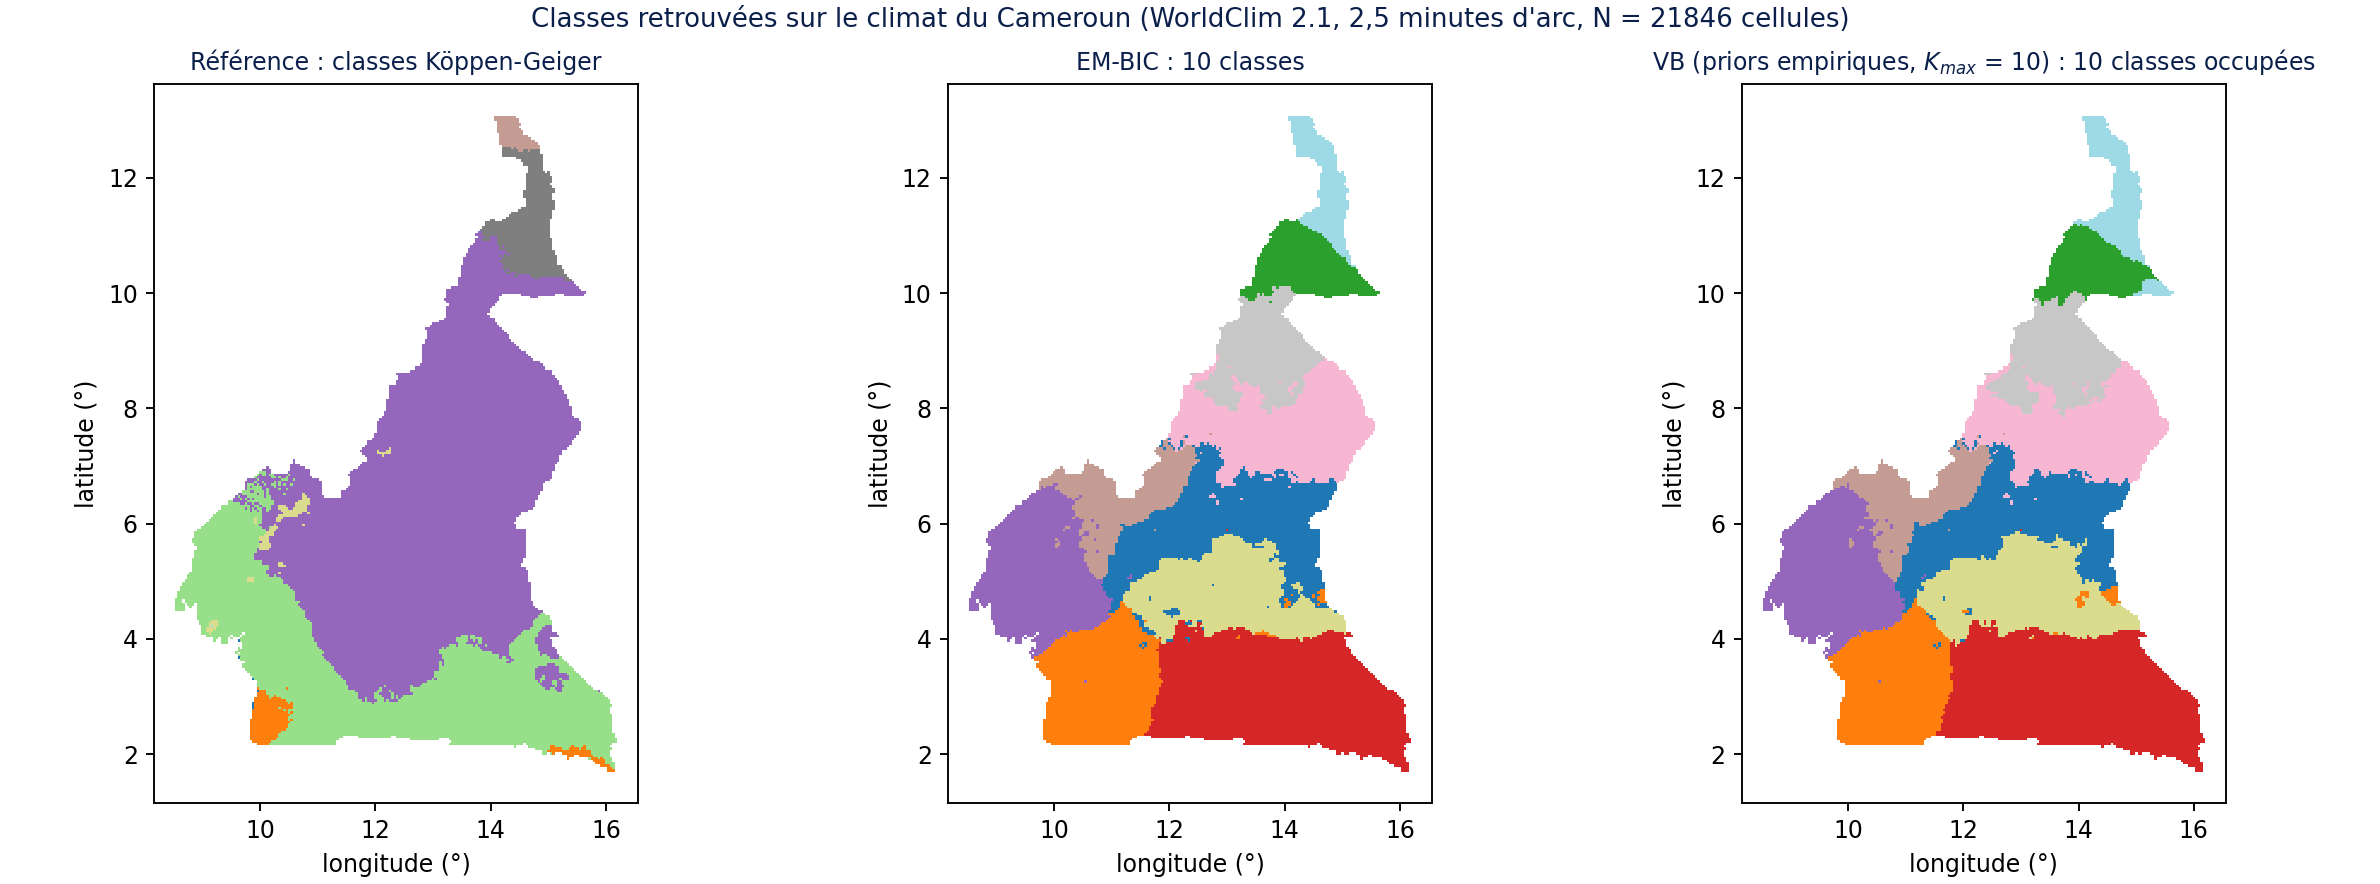
\includegraphics[width=\textwidth]{figures/climat_classes.png}
\caption{Classes de Köppen--Geiger (référence) et classes retrouvées par EM-BIC et par le VB à priors empiriques sur les 21\,846 cellules du Cameroun (WorldClim 2.1, 2,5 minutes d'arc). Contour : Natural Earth ; couleurs arbitraires, non comparables d'une carte à l'autre.}
\label{fig:climat_cartes}
\end{figure}
\begin{figure}[H]
\centering
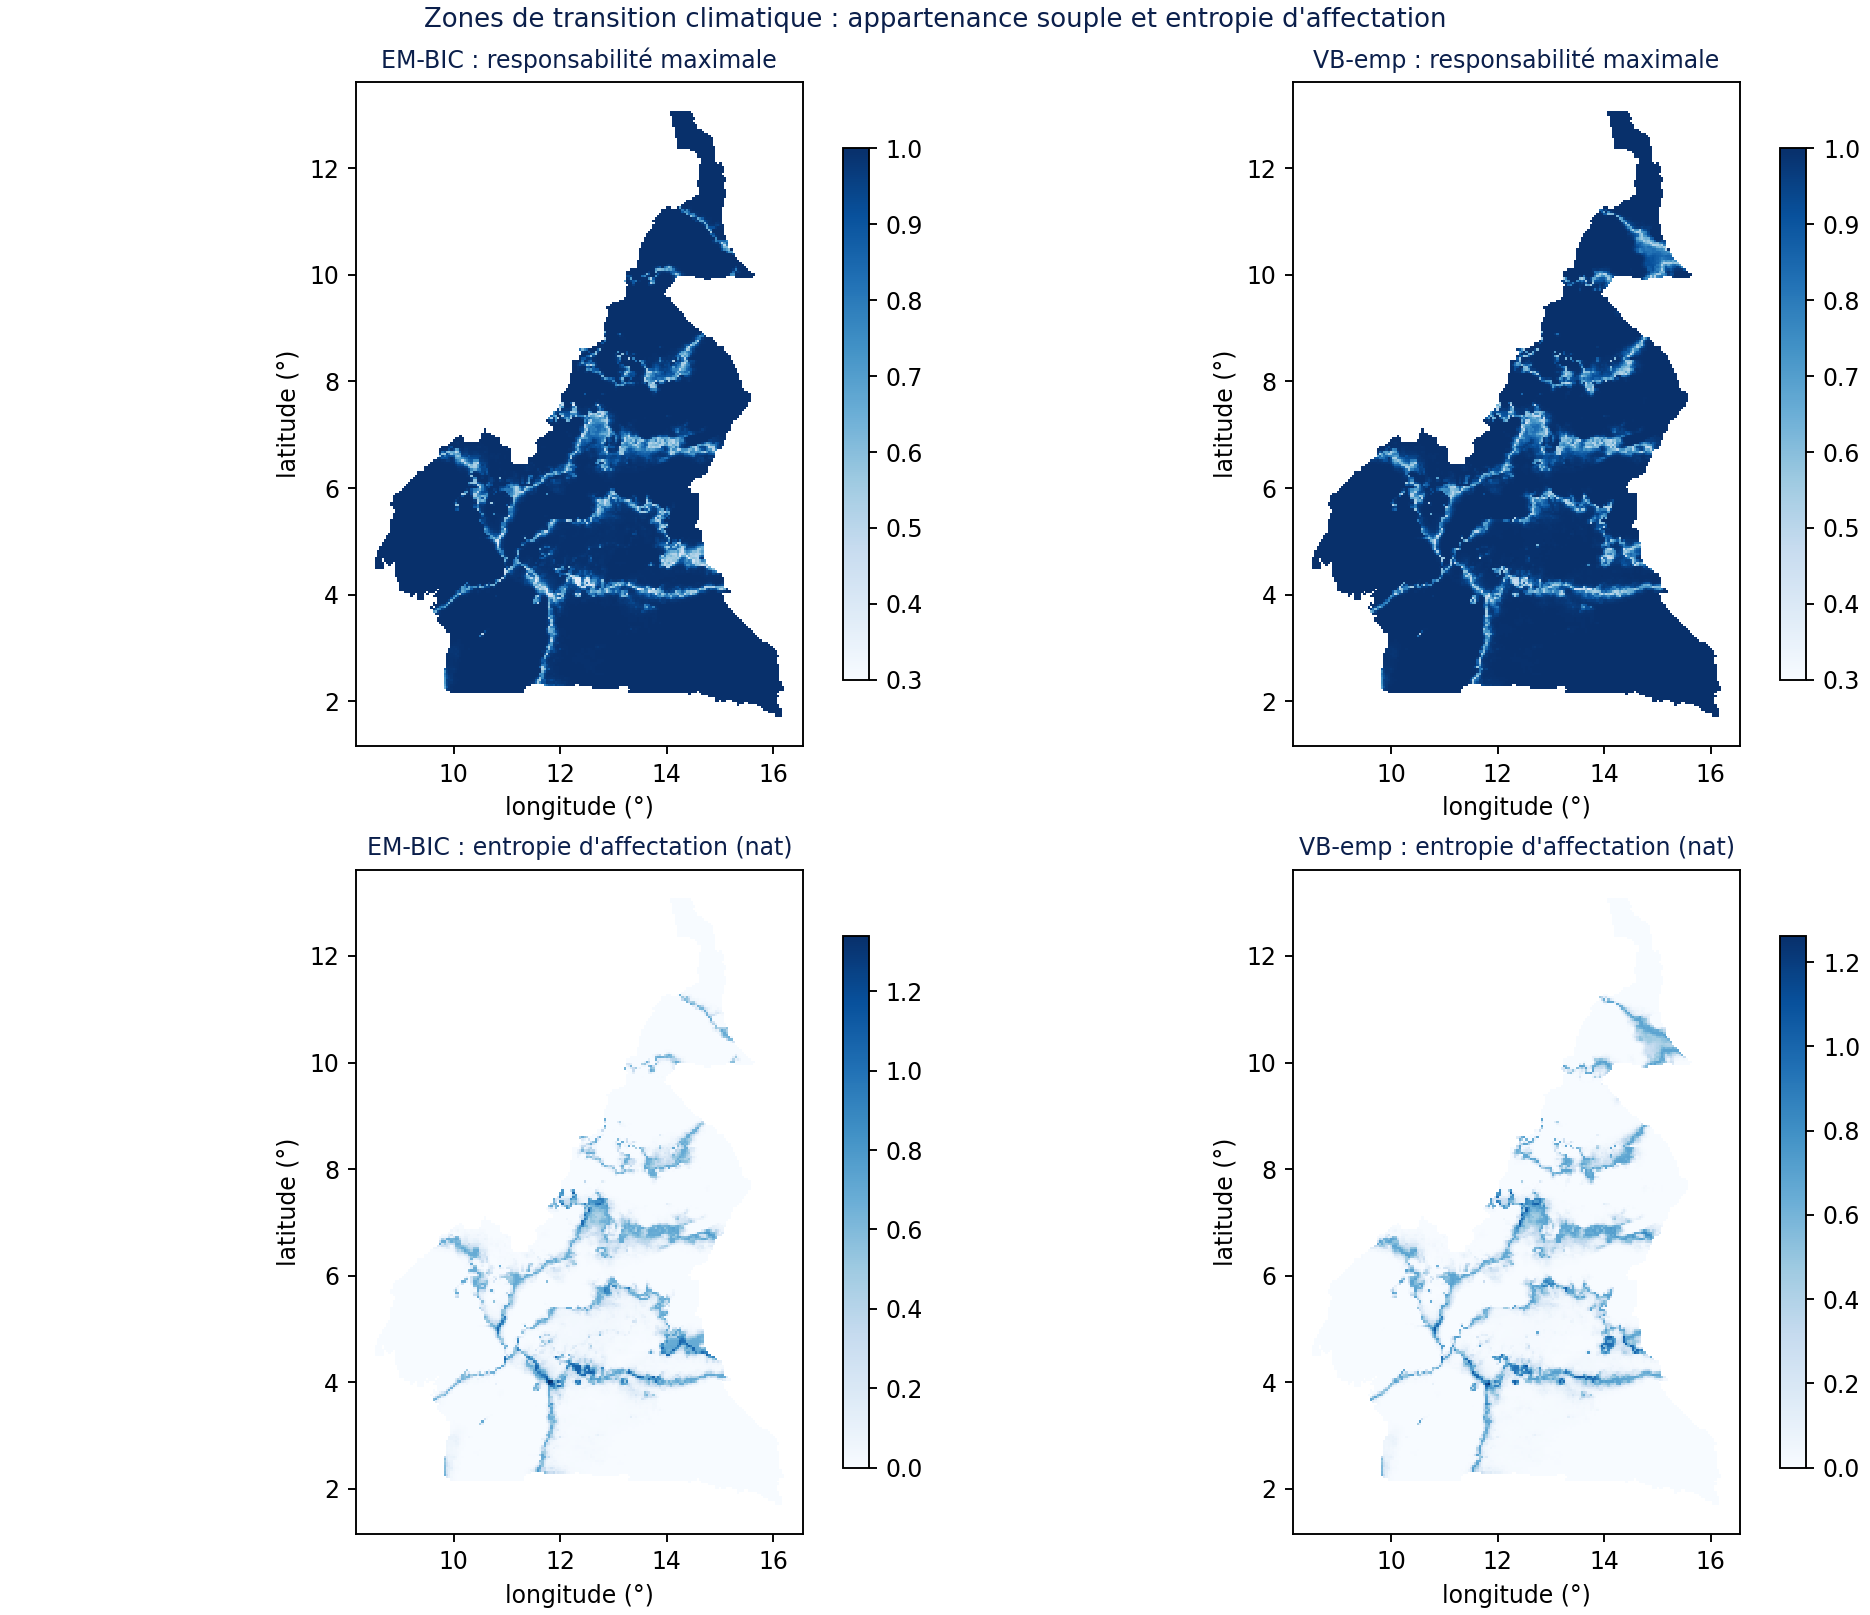
\includegraphics[width=0.9\textwidth]{figures/climat_incertitude.png}
\caption{Responsabilité maximale (haut) et entropie d'affectation (bas) de EM-BIC et du VB : les zones de transition climatique ont une entropie élevée.}
\label{fig:climat_incertitude}
\end{figure}

\textbf{Lecture. }(i) \emph{Cohérence avec le zonage.} L'ARI contre Köppen--Geiger est faible pour tous les bras et tous les effectifs (de l'ordre de 0,1 à 0,17, tableau~\ref{tab:climat_sous}) : aucune des méthodes ne retrouve la structure de Köppen--Geiger à partir de ces cinq variables, et la différence entre méthodes est petite devant ce niveau commun. La référence est définie par des seuils sur des climatologies mensuelles, non par des amas gaussiens de $(\mathrm{bio1}, \mathrm{bio4}, \log\mathrm{bio12}, \mathrm{bio15}, \text{altitude})$ ; à $N \geq 500$, BIC et ICL retiennent presque systématiquement $K_{\max} = 10$, ce qui indique que le critère continue de décroître au-delà de la plage testée (borne supérieure à repousser, non testé). Les cartes (figure~\ref{fig:climat_cartes}) montrent, pour EM-BIC comme pour le VB, des classes en bandes de latitude (gradient nord-sud) et un bloc distinct pour les hautes terres de l'Ouest, très proches d'une méthode à l'autre ; la référence Köppen--Geiger ne comporte que quelques classes très étendues sur ce territoire, ce qui est compatible avec un ARI faible pour des partitions en dix classes. À $N$ complet, le VB n'élague aucune composante ($K_{\max}=10$ toutes occupées). L'entropie d'affectation est élevée le long des limites entre bandes, c'est-à-dire dans les zones de transition climatique (figure~\ref{fig:climat_incertitude}). Le zonage agro-écologique officiel étant indisponible, la comparaison avec lui n'a pas pu être faite.

(ii) \emph{Sélection de $K$ (H1).} Sur le jeu semi-synthétique ($K_{\text{réf}}=5$), l'erreur $\lvert\hat K-5\rvert$ du VB à priors empiriques est inférieure à celle de EM-BIC et EM-ICL aux effectifs 30 et 60 (ces deux critères retiennent presque $K_{\max}$), supérieure à $N=120$, et équivalente (nulle) à $N \geq 500$, où tous retrouvent $K=5$. Le VB n'est donc pas supérieur : son avantage se limite aux très petits effectifs, où tous les ajustements sont dégénérés (H3) et où l'ARI est faible pour toutes les méthodes (tableau~\ref{tab:climat_semi}).

(iii) \emph{Qualité à grand $N$ (H2).} À $N=2\,000$ sur les données réelles, EM-BIC est supérieur au VB à priors empiriques pour l'ARI contre Köppen--Geiger (écart faible) et pour la log-vraisemblance hors bloc (écart de l'ordre de 0,3 nat par observation) : l'équivalence est rejetée dans le sens défavorable au VB. L'écart tient vraisemblablement à la flexibilité de EM-BIC, qui utilise les dix composantes avec une régularisation $\varepsilon I$, alors que les priors empiriques du VB contraignent chaque composante (explication non testée). À $N$ complet, il n'y a qu'une exécution (descriptif).

(iv) \emph{Petit $N$ et dégénérescence (H3).} Pour $N \leq 120$, presque tous les ajustements des deux familles ont au moins une composante dégénérée ($N_k < D+1$) : la différence n'est pas décidable (H3 non soutenue, tableau~\ref{tab:climat_grille}). Les VB à priors diffus sont moins touchés à $N=120$ (tableau~\ref{tab:climat_sous}), mais cette comparaison n'était pas celle qui a été fixée. En revanche, la log-vraisemblance hors bloc de l'EM est catastrophique aux petits effectifs (valeurs très négatives), alors que celle du MAP-EM et celle du VB sont incomparablement moins mauvaises (le VB, en particulier à priors diffus, étant meilleur que le MAP-EM) : les priors suffisent à stabiliser l'essentiel à stabiliser l'estimation, ce que montre déjà le MAP-EM (même régularisation, sans distribution sur $\theta$). Le VB à loi prédictive de Student a ensuite une log-vraisemblance supérieure à son évaluation plug-in aux petits effectifs : l'effet de la loi prédictive est séparé de celui des priors.

(v) \emph{Coût (H4).} Le temps médian du pipeline EM-BIC est supérieur à celui d'un VB à dix initialisations pour tous les effectifs, avec des intervalles bootstrap au-dessus de 1 (rapport de 1,1 à 4,1 selon $N$ ; à $N$ complet, une exécution donne un rapport voisin de 8). L'économie de calcul du VB sur la sélection de $K$ est donc établie ici, à la condition que la baseline soit un balayage complet avec dix initialisations par valeur de $K$.

(vi) \emph{Hyperparamètres (H5).} La variance de $\hat K$ due aux priors (plan factoriel) est supérieure à celle de EM-BIC due à l'initialisation : le VB ne supprime pas la sensibilité, il la déplace vers les hyperparamètres (expérience unique à $N=500$).

(vii) \emph{Incertitude (H6).} Voir le tableau~\ref{tab:climat_couverture} : sous-couverture des poids du VB, couverture compatible avec 90 \% pour ses moyennes, bootstrap de l'EM plus proche du nominal.

(viii) \emph{Chevauchement et dimension (H7, H8).} À $N=2\,000$, le VB à priors empiriques ne fusionne pas plus de composantes que EM-BIC ($\hat K = 5$ pour tous, hors EM-$K_{\max}$ et MAP-EM) : H7 n'est pas soutenue sur le jeu semi-synthétique ; elle n'a pas pu être testée sur les zones réelles. H8 est traitée pour la dégénérescence seule à $D=20$ (lignes H8 du tableau~\ref{tab:climat_grille}) : à $D=20$, tous les ajustements des deux familles sont dégénérés (20 sur 20 pour VB-emp comme pour EM-$K_{\max}$ à chaque effectif), de sorte que la différence est indéterminée et que \emph{H8 n'est pas soutenue}. Un résultat défavorable au VB à priors empiriques s'y ajoute : à $D=20$ son ajustement échoue numériquement (covariance non définie positive, la covariance empirique des vingt variables, très colinéaires, servant de $W_0^{-1}$) dans 80 \% des cas à $N=500$ et dans tous les cas à $N=2\,000$, alors que le VB à priors diffus ne présente aucun échec ; ces échecs sont comptés comme dégénérés. Le VB à priors diffus a aussi l'ARI le plus élevé à $D=20$ (tableau~\ref{tab:climat_sous20}). Ceci illustre la sensibilité du VB au choix des priors, par la dépendance à $W_0$ ; l'accroissement de cette dépendance avec $D$ n'a pas été testé par un plan factoriel à $D=20$.

\textbf{Conclusion du cas. }Sur ces données, le VB n'améliore ni la cohérence avec Köppen--Geiger ni la qualité à grand $N$ ; il se distingue par un pipeline moins coûteux que EM-BIC en temps total, par une stabilité de l'estimation aux petits effectifs qui est largement due à la régularisation par les priors (le MAP-EM l'obtient aussi), et par une incertitude dont la couverture est insuffisante pour les poids.

\textbf{Limites. }La dépendance spatiale viole l'hypothèse i.i.d. du mélange (l'espacement et les blocs l'atténuent sans la supprimer) ; la circularité partielle des étiquettes est traitée par le critère hors bloc ; certaines variables restent bornées ou asymétriques malgré le logarithme ; un grand nombre de cellules rend les tests très puissants, d'où les marges d'équivalence ; les résultats portent sur le Cameroun et ne se généralisent pas par défaut à l'Afrique centrale (à tester). Si le zonage officiel n'est pas disponible, seul Köppen--Geiger sert de référence.


\subsection{Cas : pLSA contre LDA sur un corpus réel}
\textbf{Niveaux d'inférence. }La LDA de Blei, Ng et Jordan (2003) est présentée à tort comme un exact analogue du GMM bayésien. Au sens de la figure~\ref{fig:trois_niveaux}, la LDA du code est un \emph{EM variationnel à $\theta$ ponctuel} : $q(\theta_d)$ est un Dirichlet (paramètres $\gamma_d$), mais les distributions de mots par thème $\beta_k$ sont des paramètres ponctuels estimés à l'étape M et $\alpha$ est fixé. Elle n'est pas un VB complet. La correspondance avec le GMM est donc partielle : $\gamma_k \leftrightarrow \alpha_k$ vaut pour les poids de mélange ($\theta_d$ joue le rôle de $\pi$ par document), mais $\beta_k$ n'a pas de prior (contrairement à $(\mu_k,\Lambda_k)$ dans le GMM bayésien). Le comparateur « EM classique » de la LDA est le pLSA (Hofmann, 1999), qui estime $\theta_d$ et $\phi_k$ par maximum de vraisemblance sans prior.

Ce placement suit le texte original. Blei, Ng et Jordan (2003, section 5.3) estiment $\alpha$ et $\beta$ par un EM variationnel de type bayes empirique : l'étape E optimise, document par document, les paramètres variationnels $\gamma_d$ de $q(\theta_d)$ et $\phi_{dn}$ de $q(z_{dn})$ ; l'étape M maximise la borne qui en résulte par rapport à $\alpha$ et $\beta$, qui restent ponctuels (niveau 2). Leur variante « lissée » (section 5.4) place un prior de Dirichlet de paramètre $\eta$ sur chaque $\beta_k$, qui devient aléatoire et reçoit un facteur variationnel. C'est cette version que reprennent Hoffman et al. (2013) : les $\beta_k$ y sont les variables \emph{globales} et les $(\theta_d, z_{dn})$ les variables \emph{locales} de la section 1.7.7, et la SVI met à jour le paramètre variationnel de $\beta$ par mini-lots de documents. La LDA lissée relève ainsi du niveau 3 pour toutes ses variables cachées, ses seuls points estimés étant les hyperparamètres $\alpha$ et $\eta$, que Blei, Ng et Jordan estiment encore par bayes empirique (section 5.4), comme le font les priors empiriques du VB de ce travail pour $m_0$ et $W_0$. La LDA du code correspond à la version non lissée, à $\alpha$ fixé et non estimé : la comparaison pLSA contre LDA mesure donc l'effet du prior sur $\theta_d$ seul, et non celui d'un traitement bayésien complet.

\begin{figure}[H]
\centering
\begin{tikzpicture}[>=Stealth,
    v/.style={circle,draw=navy,minimum size=0.9cm,font=\footnotesize,inner sep=0pt},
    o/.style={circle,draw=navy,fill=ciel!40,minimum size=0.9cm,font=\footnotesize,inner sep=0pt}]
  \node[font=\footnotesize\bfseries] at (1.7,3.0) {pLSA (EM, sans prior)};
  \node[v] (theta1) at (0,1.8) {$\theta_d$};
  \node[v] (z1) at (1.8,1.8) {$z$};
  \node[o] (w1) at (3.4,1.8) {$w$};
  \node[font=\scriptsize] (phi1) at (3.4,0.4) {$\phi_k$ ponctuel};
  \draw[->] (theta1) -- (z1);
  \draw[->] (z1) -- (w1);
  \draw[->] (phi1) -- (w1);
  \node[font=\scriptsize,text=gray] at (0,0.9) {ponctuel, sans prior};
  \node[font=\footnotesize\bfseries] at (9.4,3.0) {LDA (EM variationnel)};
  \node[font=\scriptsize] (alpha) at (6.4,1.8) {$\alpha$};
  \node[v] (theta2) at (7.8,1.8) {$\theta_d$};
  \node[v] (z2) at (9.4,1.8) {$z$};
  \node[o] (w2) at (11,1.8) {$w$};
  \node[font=\scriptsize] (beta2) at (11,0.4) {$\beta_k$ ponctuel};
  \draw[->] (alpha) -- (theta2);
  \draw[->] (theta2) -- (z2);
  \draw[->] (z2) -- (w2);
  \draw[->] (beta2) -- (w2);
  \node[font=\scriptsize,text=gray] at (7.8,0.9) {$\sim\mathrm{Dir}(\alpha)$, prior};
\end{tikzpicture}
\caption{Modèles graphiques du pLSA et de la LDA utilisée ici. La différence testée est le prior de Dirichlet sur $\theta_d$ (LDA) contre un $\theta_d$ ponctuel sans prior (pLSA). Dans les deux cas les distributions de mots par thème sont ponctuelles : la LDA du code est un EM variationnel à $\beta$ ponctuel, non un VB complet.}
\label{fig:plsa_lda}
\end{figure}


\textbf{Hypothèse, fixée avant l'analyse. }Le pLSA sur-apprend davantage que la LDA quand le nombre de documents $N$ est petit (le prior de Dirichlet sur $\theta_d$ est la raison d'être de la LDA) ; l'écart se réduit quand $N$ croît. Elle est testée par la différence appariée, par $N \in \{50, 200, 1\,000\}$, de l'écart relatif entre perplexité hors échantillon et perplexité sur les documents d'apprentissage.

\textbf{Données et protocole. }Sous-ensemble de 20 Newsgroups (quatre groupes : \texttt{sci.space}, \texttt{rec.sport.baseball}, \texttt{talk.politics.mideast}, \texttt{comp.graphics}), obtenu par \texttt{sklearn.datasets.fetch\_20newsgroups} ; jeu de diffusion libre pour la recherche, sans licence explicite (à citer : Lang, 1995). Prétraitement : minuscules, suppression des en-têtes, citations et signatures, ponctuation et chiffres, mots vides (liste anglaise de scikit-learn), racinisation de Porter, vocabulaire de 1\,500 mots présents dans au moins cinq documents. La perplexité hors échantillon est calculée par complétion de document (la moitié des mots d'un document sert à estimer $\theta_d$, l'autre à l'évaluer, de façon identique pour les deux modèles) ; la cohérence des thèmes est mesurée par le NPMI des dix premiers mots ; la pureté est calculée par rapport aux étiquettes du corpus. Les deux modèles partagent le critère d'arrêt de la figure~\ref{fig:boucle_arret}. Les probabilités sont planchées à $10^{-12}$ et la part de mots planchés est rapportée.

\tableauGenere{texte_plsa_lda}
\tableauGenere{texte_grille}

\textbf{Lecture. }L'hypothèse est soutenue en ce qui concerne le surapprentissage mesuré par l'écart relatif entre perplexité hors échantillon et perplexité d'apprentissage : le pLSA sur-apprend davantage que la LDA à chaque taille, l'écart relatif diminue quand $N$ croît, et la différence appariée (pLSA moins LDA) est significative aux trois tailles (tableau~\ref{tab:texte_grille} ; la plus petite probabilité critique atteignable avec 10 réplications est de 0,005). À $N=50$, la perplexité hors échantillon du pLSA est plus de sept fois celle de la LDA, avec une part de mots à probabilité nulle (plancher) de l'ordre de 12 \%. En revanche, le pLSA n'est pas moins bon en tout : à $N=1\,000$, sa perplexité hors échantillon est \emph{inférieure} à celle de la LDA, et sa cohérence NPMI et sa pureté sont supérieures à celles de la LDA aux trois tailles (tableau~\ref{tab:texte}). Deux réserves s'imposent. D'abord, la LDA du code lisse $\beta$ (constante de lissage de $10^{-3}$) et le pLSA ne le fait pas ; une partie de l'écart à $N=50$ vient des probabilités nulles du pLSA et non seulement du prior sur $\theta_d$. Ensuite, une part des exécutions du pLSA n'est pas convergée au plafond de 150 étapes M (colonne « Non convergés »), et seules dix réplications par taille ont été faites.

Cette expérience remplace la démonstration sur douze phrases des versions précédentes de ce travail, qui ne comparait pas deux algorithmes et dont les thèmes étaient instables. Le corpus de test est un seul tirage de 600 documents ; les résultats dépendent du prétraitement et du nombre de thèmes ($K=4$, égal au nombre de groupes), ce qui borne leur portée.


\subsection{Domaines d'usage : vision, bio-informatique (revue de la littérature)}
Ces deux domaines ne font l'objet d'aucune expérience dans ce mémoire. Ce qui suit est une revue : toute affirmation sans source est marquée « non testé ».

\textbf{Vision par ordinateur. }Les mélanges gaussiens servent à la segmentation d'images (chaque pixel est décrit par sa couleur ou une texture, $D=3$ ou davantage) ; le nombre $N$ de pixels peut dépasser le million, ce qui replace la scalabilité au centre du choix de l'algorithme. Dans l'algorithme de soustraction de fond de Stauffer et Grimson (1999), chaque pixel est modélisé par un petit mélange de gaussiennes mis à jour de façon incrémentale par une heuristique inspirée de l'EM online (et non exactement l'EM online) : le taux d'apprentissage $\rho$ est fixé et les composantes de poids élevé et de faible variance sont classées comme fond. Cette règle utilise l'interprétation des poids comme fréquences d'occurrence (section 1.6.2.c). L'affirmation que l'EM classique convient mieux au temps réel et l'EM variationnel à la segmentation hors ligne n'a pas été testée ici : \emph{non testé}.

\textbf{Bio-informatique. }Les modèles de mélange servent à identifier des sous-populations dans des données d'expression génique (cellule unique), pour lesquelles le nombre de sous-populations est souvent l'objet de l'étude. La dimension ($D$ de l'ordre du millier de gènes) rend la covariance pleine impraticable pour les deux algorithmes : le coût est en $KD^3$ et les effectifs $N_k < D+1$ conduisent à des covariances singulières (section 2.5). En pratique la dimension est réduite au préalable ou les covariances sont contraintes (diagonales). Les mélanges infinis (processus de Dirichlet, Rasmussen, 2000) constituent un mécanisme différent du VB à $K_{\max}$ fini étudié ici. L'affirmation selon laquelle l'EM variationnel serait « largement préféré » dans ce domaine n'est ni sourcée ni testée ici : \emph{non testé}. Les modèles de Markov cachés ajustés par Baum-Welch (section 1.6.6) restent une référence pour l'annotation de séquences, sans que ce mémoire en mesure les délais pour des génomes entiers : \emph{non testé}.


\subsection{Cas secondaire : rendements du S\&P 500 et risque de marché}
Le rendement d'un actif est $r_t = 100\,\ln(P_t/P_{t-1})$, en pourcentage. La loi de ces rendements a des queues plus épaisses qu'une gaussienne ; un mélange de gaussiennes les représente, et le VB propose en outre une loi sur les paramètres, d'où une loi prédictive de Student et un intervalle de crédibilité de la VaR. Ce cas est secondaire : la période d'évaluation (de janvier 2022 à octobre 2026) diffère fortement de la période d'apprentissage (octobre 2016 à décembre 2021, krach de 2020 compris) ; la kurtosis excédentaire des deux périodes (tableau~\ref{tab:3_cas_desc}) est calculée par le code. Toute VaR calée sur la période 2020 est prudente par construction sur une période plus calme : le backtest mesure alors autant le changement de régime que la qualité de l'algorithme.

\textbf{Hypothèses, fixées avant l'analyse. }(H4) Un mélange ($K>1$) a une log-vraisemblance moyenne hors échantillon supérieure à celle de la gaussienne unique et de la Student-t ; décidée par un test de Diebold--Mariano avec la correction de Harvey, Leybourne et Newbold, sur les log-scores quotidiens. (H5) La VaR gaussienne à 1 \% est franchie plus souvent que prévu, ce que l'on décide par le test de Kupiec au seuil de 5 \% ; l'écart entre mélange EM et mélange VB est, lui, une question descriptive (de l'ordre d'une exception) et ne s'interprète pas comme une différence d'algorithme. (H6) L'intervalle de crédibilité de la VaR du VB est disponible sans calcul supplémentaire ; l'intervalle bootstrap de l'EM (au moins 1\,000 réplicats) mesure un autre objet (variabilité d'estimateur) et la comparaison de leurs largeurs n'est pas une comparaison de fiabilité.

\textbf{Ce qui est comparé. }Gaussienne, Student-t, GARCH(1,1) à innovations de Student, simulation historique, mélange EM (K choisi par le BIC), VB en évaluation plug-in (paramètres $\mathbb{E}[\pi_k], m_k, (\mathbb{E}[\Lambda_k])^{-1}$) et en loi prédictive de Student, et un HMM à deux états en filtrage \emph{forward} (aucune information future). La différence entre l'évaluation prédictive et l'évaluation plug-in d'un même VB isole l'effet de la loi prédictive de celui de l'inférence bayésienne. Les modèles sont ajustés une seule fois sur l'apprentissage puis figés, sans réestimation glissante. La VaR et l'ES de la prédictive de Student sont obtenues par simulation de 200\,000 tirages du mélange de Student (erreur de Monte Carlo en $1/\sqrt{np}$). Le backtest comprend les tests de Kupiec, de Christoffersen (indépendance et couverture conditionnelle) et le test de l'ES d'Acerbi et Székely (2014) (statistiques $Z_1$ et $Z_2$, positives en cas de risque sous-estimé).

\tableauGenere{sp500_descriptif}
\tableauGenere{sp500_backtests}
\tableauGenere{sp500_diebold_mariano}
\tableauGenere{sp500_intervalles}

\begin{figure}[H]
\centering
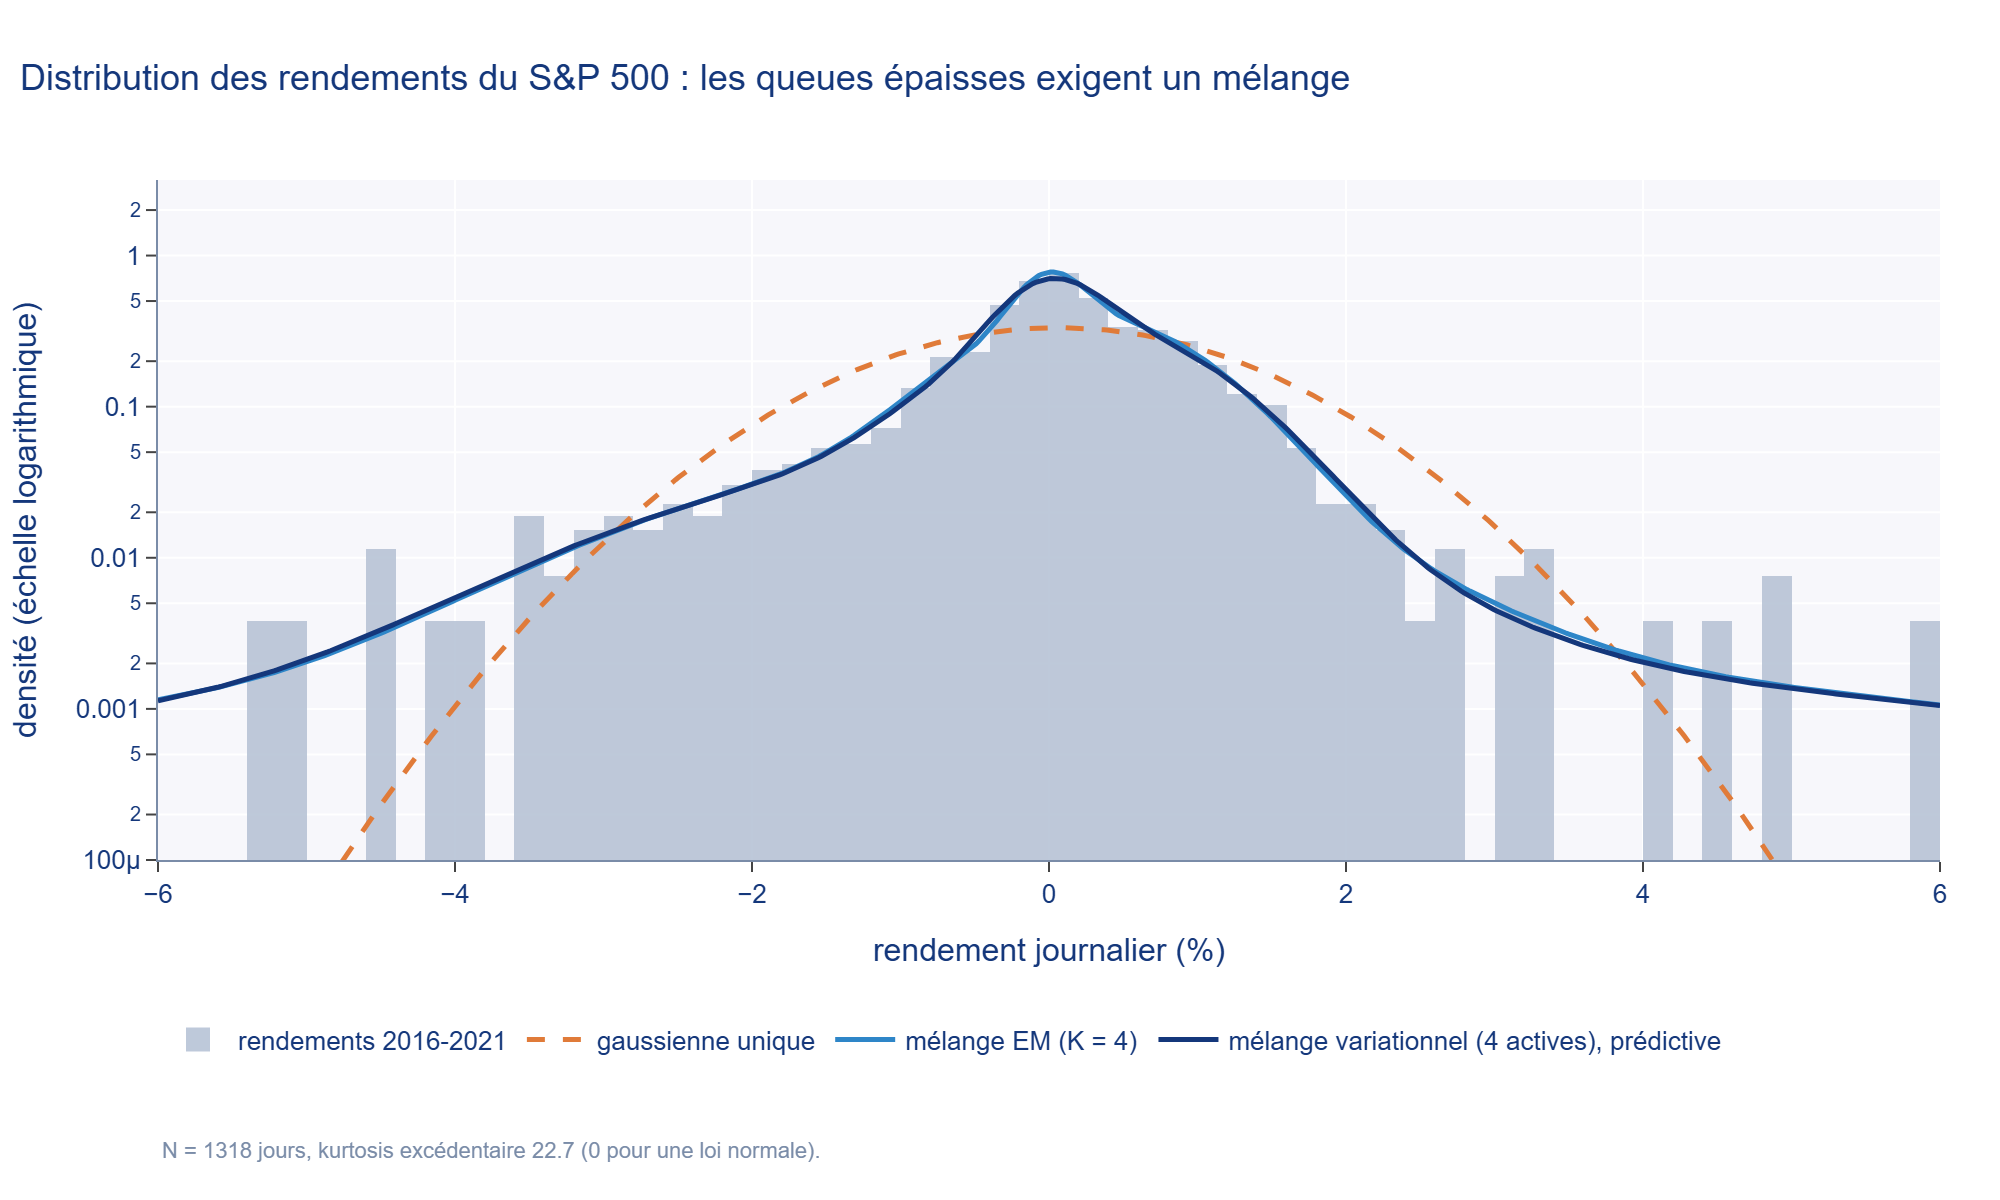
\includegraphics[width=0.95\textwidth]{figures/fig13.png}
\caption{Distribution des rendements quotidiens du S\&P 500 sur la période d'apprentissage et densités ajustées (échelle logarithmique de la densité). Source : série FRED SP500 (S\&P Dow Jones Indices), archive \texttt{data/sp500\_fred.csv}.}
\label{fig:3_cas_dist}
\end{figure}
\begin{figure}[H]
\centering
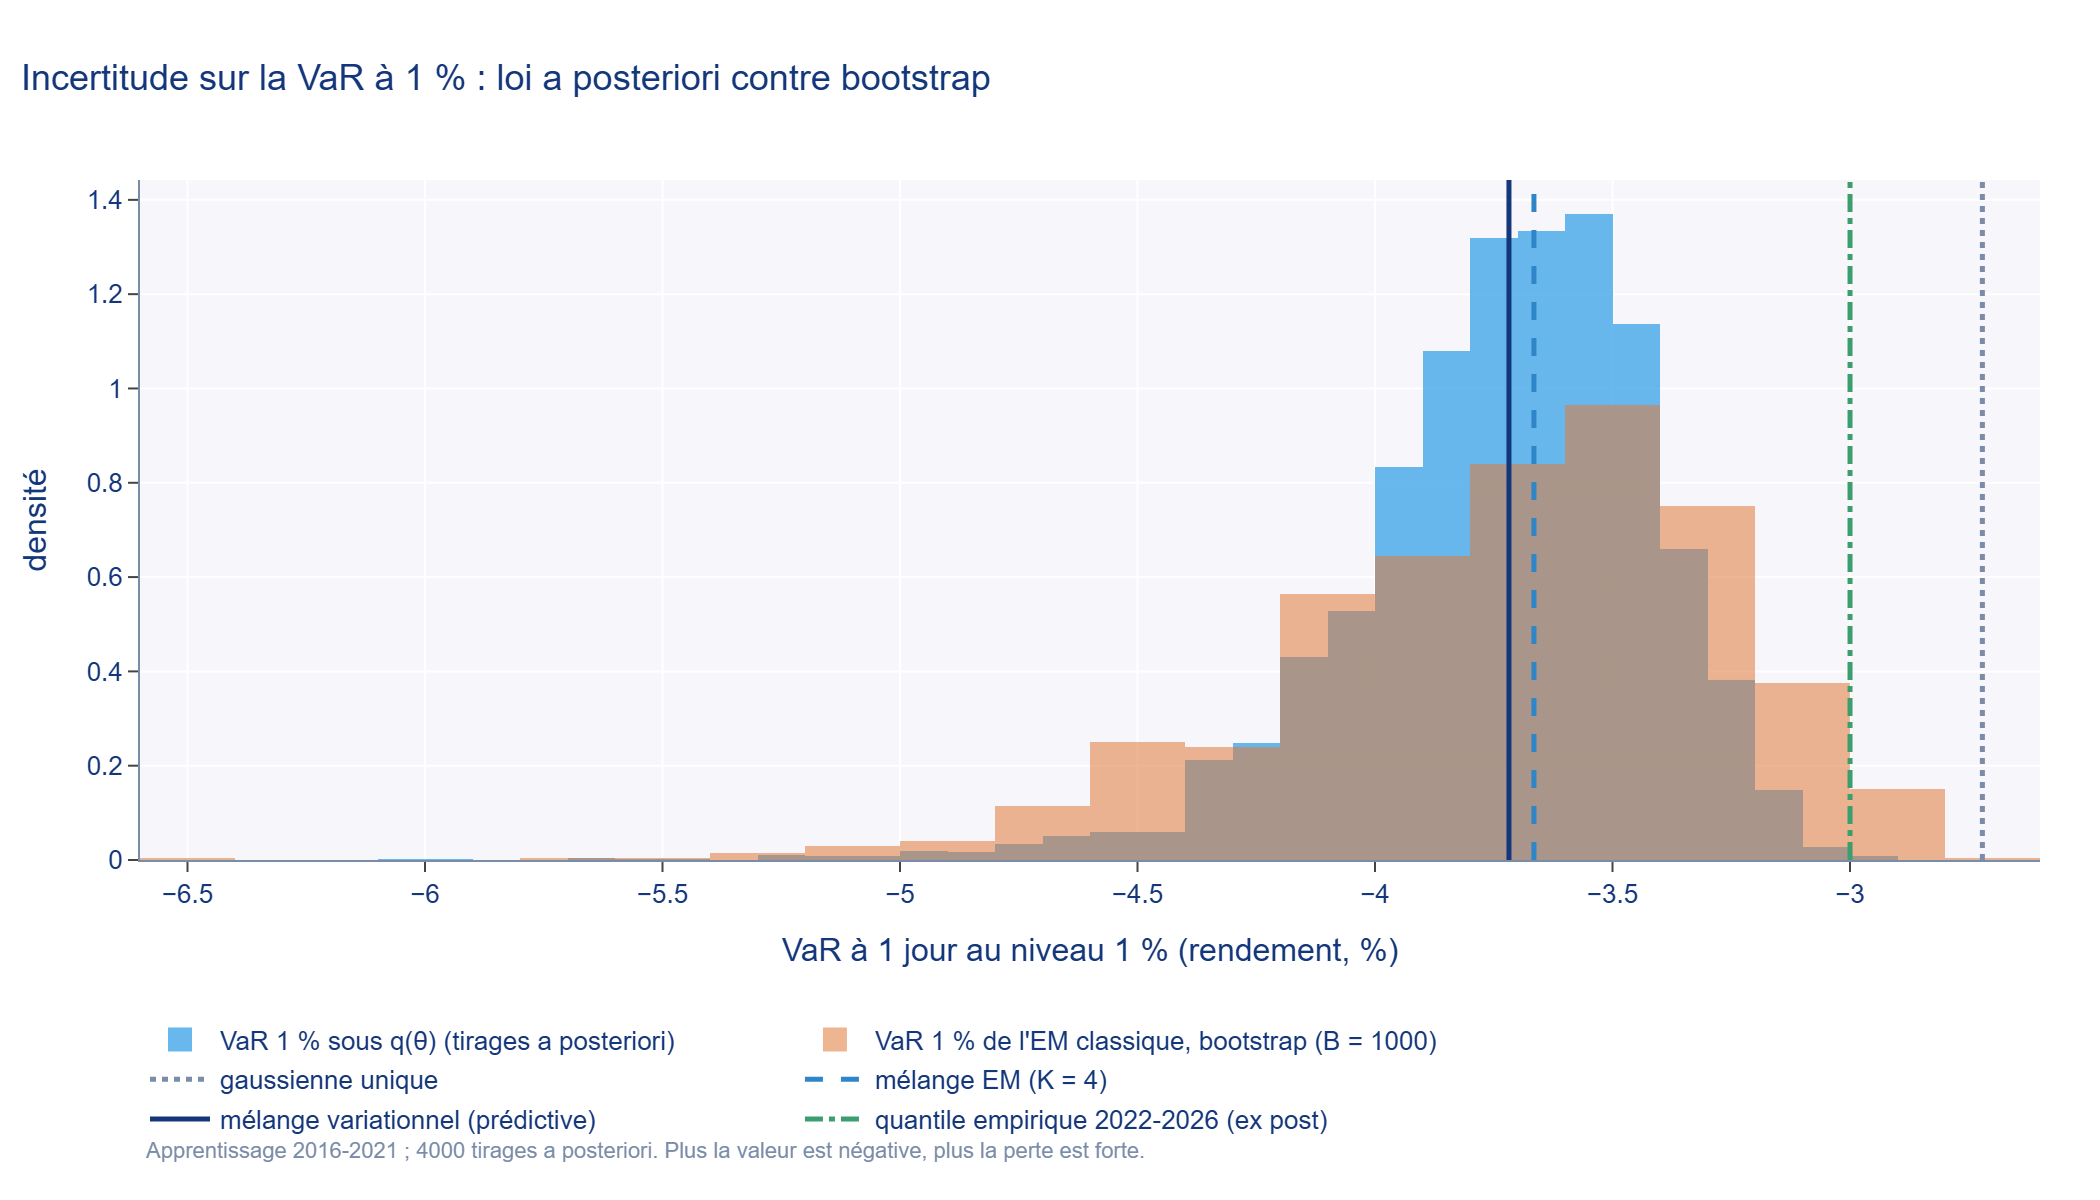
\includegraphics[width=0.95\textwidth]{figures/fig15.png}
\caption{Incertitude sur la VaR à 1 \% : tirages a posteriori sous la loi variationnelle et bootstrap non paramétrique de l'EM classique. Les deux distributions ne mesurent pas le même objet.}
\label{fig:3_cas_var}
\end{figure}

\textbf{Lecture. }(H4) Les mélanges (EM-BIC à $K=4$ en plug-in, VB en loi prédictive) et la loi de Student obtiennent une log-vraisemblance moyenne hors échantillon supérieure à celle de la gaussienne d'environ 0,04 à 0,05 nat par jour ; les tests de Diebold--Mariano (tableau~\ref{tab:sp500_dm}) ne rejettent pas l'égalité au seuil de 5 \% (probabilités critiques de 0,08 à 0,12, supérieures après correction de Holm) : \emph{H4 n'est pas soutenue}, la direction est celle attendue mais l'écart n'est pas significatif. Le GARCH(1,1) à innovations de Student est nettement supérieur à tous les modèles i.i.d., mélanges compris. L'évaluation prédictive du VB ne diffère pas de son évaluation plug-in (différence nulle à la précision du tableau, DM non significatif) : l'avantage supposé de la loi prédictive n'apparaît pas sur ces données.

(H5) La VaR gaussienne à 1 \% est franchie 20 fois pour 11,9 attendues, et le test de Kupiec la rejette au seuil de 5 \% (probabilité critique de 0,032) : H5 est soutenue. À 1 \%, les mélanges sont trop prudents (5 ou 6 exceptions pour 11,9 attendues) ; le test de Kupiec rejette la prédictive du VB (5 exceptions) mais pas le plug-in du VB ni l'EM (6 exceptions, probabilité critique de 0,056) : une exception d'écart suffit à franchir le seuil, de sorte que l'affirmation antérieure « VB mieux calibré à 1 \% » est retirée. À 5 \%, les mélanges sont bien calibrés (Kupiec non rejeté) alors que la gaussienne est trop prudente (41 exceptions pour 59,7 attendues) ; la Student et le GARCH-t sont, eux, trop souvent franchis à 5 \% (Kupiec rejeté). Le test d'indépendance de Christoffersen rejette à 1 \% la gaussienne, la Student, la simulation historique, EM et VB (exceptions groupées), et ne rejette ni le GARCH-t ni le HMM filtré, dont la couverture conditionnelle n'est pas rejetée. Pour l'ES (Acerbi--Székely), les statistiques $Z_2$ des mélanges, de la Student et de la simulation historique sont négatives à 1 \% (ES surestimée, prudence) et celle de la gaussienne positive (queue sous-estimée) ; elles ne sont pas accompagnées de probabilité critique.

Ces résultats se lisent avec le changement de régime : la kurtosis excédentaire passe de 22,7 (apprentissage, krach de 2020 compris) à 6,5 (évaluation), de sorte qu'une VaR calée sur 2016-2021 est prudente par construction. Les modèles à volatilité conditionnelle (GARCH-t, HMM filtré) sont les mieux calibrés à 1 \% (couverture conditionnelle non rejetée) : la volatilité en grappes explique plus que le choix entre EM et VB.

(H6) L'intervalle de crédibilité à 95 \% de la VaR à 1 \% du VB est plus étroit que l'intervalle bootstrap de l'EM (1 000 réplicats) d'environ un tiers, aux deux niveaux (tableau~\ref{tab:sp500_int}). Les deux objets diffèrent et la couverture n'est pas évaluée sur ces données ; elle l'est, pour les poids et les moyennes, sur le jeu semi-synthétique du cas climatique, où le VB sous-couvre les poids.


\subsection{Systèmes de recommandation (revue de la littérature)}
Dans les systèmes de recommandation, la factorisation matricielle probabiliste place des priors gaussiens sur les vecteurs latents d'utilisateurs et d'articles, et l'inférence variationnelle donne une loi a posteriori exploitable pour l'exploration (échantillonnage de Thompson). L'intérêt de cette incertitude pour le démarrage à froid est une hypothèse de la littérature : \emph{non testé} ici, aucune expérience de recommandation n'ayant été conduite.

\begin{table}[H]
\centering
\small
\setlength{\tabcolsep}{0.14cm}
\begin{tabular}{|p{3.6cm}|p{5.4cm}|p{5.2cm}|}
\hline
\textbf{Domaine} & \textbf{Usage décrit} & \textbf{Statut de la preuve dans ce mémoire} \\
\hline
Climat (cas principal) & Régimes climatiques, mélanges gaussiens & Expériences répliquées (section 3.1.1) \\
\hline
Texte & Modèles de thèmes (pLSA, LDA) & Expérience répliquée sur corpus réel \\
\hline
Finance & VaR, ES, régimes de marché & Expérience unique sur un indice, période de test non stationnaire \\
\hline
Vision & Segmentation, soustraction de fond & Revue : non testé \\
\hline
Bio-informatique & Sous-populations cellulaires, annotation de séquences & Revue : non testé \\
\hline
Recommandation & Factorisation matricielle probabiliste, démarrage à froid & Revue : non testé \\
\hline
\end{tabular}
\caption{Statut de la preuve par domaine d'application}
\label{tab:3_1}
\end{table}

\section{Implémentation de l'EM classique}
L'EM classique est implémenté en PyTorch à partir des équations du chapitre 1, sans bibliothèque de modélisation : seules les opérations élémentaires (algèbre linéaire, factorisation de Cholesky, fonction digamma) sont utilisées, et les critères d'évaluation (BIC, AIC, indice de Rand ajusté, silhouette) sont écrits explicitement. Le code complet figure à l'annexe A ; les extraits ci-dessous montrent la correspondance avec les équations.

\subsection{Étapes E et M}
La densité gaussienne est évaluée par la factorisation de Cholesky de la covariance (section 2.2.2), puis l'étape E calcule les responsabilités en log-espace avec l'astuce du log-sum-exp (équations 1.15 et 1.18). L'étape M applique les mises à jour de l'équation (1.16).

\begin{lstlisting}[language=Python]
def logsumexp_stable(a: Tensor, dim: int = 1, keepdim: bool = True) -> Tensor:
    """Équation (1.18) : log sum exp(a_k) = a_max + log sum exp(a_k - a_max)."""
    a_max = a.max(dim=dim, keepdim=True).values
    out = a_max + torch.log(torch.exp(a - a_max).sum(dim=dim, keepdim=True))
    return out if keepdim else out.squeeze(dim)

def log_gauss(X: Tensor, mu: Tensor, cov: Tensor) -> Tensor:
    """log N(x | mu, cov) pour toutes les lignes de X, via Cholesky (section 2.2.2)."""
    D = X.shape[1]
    L = torch.linalg.cholesky(cov)
    z = torch.linalg.solve_triangular(L, (X - mu).T, upper=False)
    logdet = 2.0 * torch.log(torch.diagonal(L)).sum()
    return -0.5 * (D * LOG2PI + logdet + (z ** 2).sum(dim=0))

def _etape_e(X, pi, mu, cov):
    """Étape E (1.15) en log-espace : retourne (r, log p(x_i | theta))."""
    K = len(pi)
    log_r = torch.stack([torch.log(pi[k] + 1e-300) + log_gauss(X, mu[k], cov[k])
                         for k in range(K)], dim=1)
    log_norm = logsumexp_stable(log_r, dim=1)
    return torch.exp(log_r - log_norm), log_norm.squeeze(1)

def _etape_m(X, r, cov_type, reg):
    """Étape M (1.16) : pi_k = N_k/N, mu_k = moyenne pondérée, Sigma_k = covariance pondérée."""
    N = X.shape[0]
    Nk = r.sum(0) + 1e-10
    pi = Nk / N
    mu = (r.T @ X) / Nk[:, None]
    cov = _covariances_em(X, r, mu, Nk, cov_type, reg)
    return pi, mu, cov
\end{lstlisting}
\begin{center}\small\emph{Extrait de code : étapes E et M de l'EM classique (équations 1.15, 1.16 et 1.18)}\end{center}

\subsection{Initialisation, relances et critère d'arrêt}
Deux initialisations sont disponibles : par k-means (avec initialisation k-means++), qui donne un point de départ proche de la solution, et aléatoire (K points de données tirés au hasard et covariance globale, section 1.6.2.a). L'algorithme est relancé n\_init fois et la solution de plus grande log-vraisemblance est conservée. Le critère d'arrêt est celui de la figure~\ref{fig:boucle_arret}, commun à l'EM, au MAP-EM, au VB et au pLSA : variation relative du critère \emph{total} inférieure à $10^{-6}$, plafond de 500 étapes M, la sortie rapportant \texttt{converge} (faux si le plafond est atteint : l'exécution est alors « non convergée »). Chaque covariance reçoit $+\,\varepsilon I$, $\varepsilon = 10^{-6}$ (constante \texttt{REG\_EM}) : l'EM utilisé dans ce mémoire est donc régularisé, ce qui en fait un maximum local de la vraisemblance régularisée (section 1.6.3.a). Le code retourne aussi l'ICL, l'entropie des affectations et un indicateur de dégénérescence.

\begin{lstlisting}[language=Python]
def _em_une_fois(X, K, cov_type, n_iter, tol, reg, init, graine, prior=None):
    N, D = X.shape
    pi, mu, cov = _init_em(X, K, cov_type, init, graine, reg)
    hist, converge, n_m = [], False, 0
    while True:
        r, log_norm = _etape_e(X, pi, mu, cov)
        hist.append(float(log_norm.sum()))
        if len(hist) > 1 and a_converge(hist[-2], hist[-1], tol):
            converge = True
            break
        if n_m >= n_iter:
            break
        pi, mu, cov = _etape_m(X, r, cov_type, reg)
        n_m += 1
    return {"pi": pi, "mu": mu, "cov": cov, "r": r, "loglik": hist[-1],
            "ll_hist": hist, "n_iter": n_m, "converge": converge}
\end{lstlisting}
\begin{center}\small\emph{Extrait de code : boucle de l'EM classique avec test d'arrêt}\end{center}

\section{Implémentation de l'EM variationnel}
L'EM variationnel pour le GMM bayésien est implémenté de la même façon. Les espérances nécessaires (équations 1.29 et 1.30) sont calculées avec la fonction digamma de PyTorch, les mises à jour suivent les équations (1.26) et (1.28), et l'ELBO de l'équation (1.31) est évaluée exactement à chaque itération (annexe B).

\subsection{Étapes E et M variationnelles}
\begin{lstlisting}[language=Python]
def _attendus(P, D):
    """E[ln|Lambda_k|] (1.29) et E[Lambda_k] pour chaque composante."""
    if P["cov_type"] in ("full", "tied"):
        i = torch.arange(1, D + 1, dtype=torch.float64)
        Elogdet = (torch.special.digamma((P["nu"][:, None] + 1 - i) / 2).sum(-1)
                   + D * LN2 + torch.logdet(P["W"]))
        Elam = P["nu"][:, None, None] * P["W"]
    else:
        psi = torch.special.digamma(P["a"]) - torch.log(P["b"])
        Elogdet = psi.sum(-1)
        Elam = torch.diag_embed(P["a"] / P["b"])
    return Elogdet, Elam

def _etape_e_var(X, P):
    """Étape E variationnelle, équation (1.27), avec la forme quadratique (1.30)."""
    N, D = X.shape
    Elogpi = torch.special.digamma(P["alpha"]) - torch.special.digamma(P["alpha"].sum())
    Elogdet, Elam = _attendus(P, D)
    diff = X[None, :, :] - P["m"][:, None, :]
    quad = D / P["beta"][None, :] + torch.einsum("knd,kde,kne->nk", diff, Elam, diff)
    log_rho = Elogpi[None] + 0.5 * Elogdet[None] - 0.5 * D * LOG2PI - 0.5 * quad
    log_norm = logsumexp_stable(log_rho, dim=1)
    return torch.exp(log_rho - log_norm), log_norm.squeeze(1)
\end{lstlisting}
\begin{center}\small\emph{Extrait de code : étape E variationnelle (équations 1.27, 1.29 et 1.30)}\end{center}
\begin{lstlisting}[language=Python]
def _etape_m_var(Nk, xbar, Sk, pr: PrioriNW, cov_type):
    """Étape M variationnelle, équations (1.26) et (1.28), plus les variantes de covariance."""
    K, D = xbar.shape
    beta = pr.beta0 + Nk
    m = (pr.beta0 * pr.m0 + Nk[:, None] * xbar) / beta[:, None]
    d0 = xbar - pr.m0
    terme_prior = (pr.beta0 * Nk / (pr.beta0 + Nk))
    sc = Nk[:, None, None] * Sk + terme_prior[:, None, None] * d0[:, :, None] * d0[:, None, :]
    P = {"alpha": pr.alpha0 + Nk, "beta": beta, "m": m, "cov_type": cov_type}
    if cov_type == "full":
        P["nu"] = pr.nu0 + Nk
        P["Winv"] = pr.W0inv[None] + sc
        P["W"] = torch.linalg.inv(P["Winv"])
    elif cov_type == "tied":
        P["nu"] = torch.full((K,), pr.nu0 + float(Nk.sum()))
        Winv = pr.W0inv + sc.sum(0)
        P["Winv"] = Winv.expand(K, D, D).clone()
        P["W"] = torch.linalg.inv(Winv).expand(K, D, D).clone()
    else:                                       # diag, spherical : priors Gamma sur les précisions
        a0 = pr.nu0 / 2.0
        b0 = 0.5 * torch.diagonal(pr.W0inv)
        sd = torch.diagonal(sc, dim1=1, dim2=2)
        if cov_type == "diag":
            P["a"] = (a0 + Nk / 2.0)[:, None].expand(K, D).clone()
            P["b"] = b0[None] + 0.5 * sd
        else:
            P["a"] = (a0 + D * Nk / 2.0)[:, None].expand(K, D).clone()
            P["b"] = (b0.mean() + 0.5 * sd.sum(1))[:, None].expand(K, D).clone()
    return P
\end{lstlisting}
\begin{center}\small\emph{Extrait de code : étape M variationnelle (équations 1.26 et 1.28 pour la covariance pleine)}\end{center}

Les variantes de covariance tied, diag et spherical, absentes du chapitre 1, sont obtenues avec un prior de Wishart partagé ou des priors Gamma sur les précisions. Leur ELBO n'est ni dérivé ni implémenté : le critère d'arrêt est la somme des log-normalisations de l'étape E, c'est-à-dire l'ELBO privé du terme $\mathrm{KL}[q(\theta)\Vert p(\theta)]$, qui n'est pas nécessairement monotone. Ces variantes sont donc une \emph{approximation} (clé \texttt{critere\_nom} = \texttt{approximation\_log\_norm}) et les conclusions qui les concernent sont formulées en conséquence ; le terme $D/\beta_k$ de l'étape E reste exact pour ces priors.

\subsection{Effet de l'initialisation et des priors}
Le tableau~\ref{tab:init_priors} compare, sur le jeu de données de référence (K = 6, graine 42), les stratégies d'initialisation et les deux jeux de priors de la section 2.3.1.

\tableauGenere{init_priors}
Deux enseignements se dégagent du tableau~\ref{tab:init_priors}. D'abord, l'initialisation aléatoire exige plus d'itérations que k-means ; une exécution du VB qui atteint le plafond de 500 étapes M est marquée « non convergée » et n'est pas un résultat à interpréter comme les autres. Ensuite, le résultat qualitatif dépend des priors : le VB déplace la sensibilité de l'initialisation vers les hyperparamètres (sections 1.7.4 et 2.3.14).

\section{Résultats expérimentaux et discussion}
L'exécution du protocole du chapitre 2 avec ces implémentations produit les tableaux de la section 2.3, générés par le code et non saisis à la main ; ce chapitre n'en reprend pas les valeurs.

Les limites identifiées à la section 1.7.9 (sensibilité aux hyperparamètres du prior, surcoût de calcul, dépendance à $K_{\max}$, irréversibilité de l'élagage) s'appliquent ; les variantes stochastiques (SVI, EM online) répondent à la question de la taille des données pour les deux algorithmes.

\subsection{Synthèse consolidée de l'ensemble des résultats expérimentaux}
Le tableau~\ref{tab:2_17} (grille « axe $\times$ preuve ») consolide les résultats du chapitre 2 et des cas du présent chapitre ; chaque valeur numérique y est lue dans un fichier produit par le code et chaque ligne porte son niveau de preuve.

Cette synthèse ne désigne pas un algorithme supérieur. Elle montre que l'élagage et la quantification d'une incertitude approchée par le VB ont une contrepartie documentée (sensibilité aux priors et à $K_{\max}$, coût par ajustement, couverture à vérifier), et que plusieurs inconvénients restent « non testés ». Les conclusions s'arrêtent à ce que les niveaux de preuve de la grille autorisent.

\section{Recommandations pratiques}
À l'issue de l'ensemble des analyses théoriques, expérimentales et applicatives conduites dans ce mémoire, cette section propose une synthèse opérationnelle, destinée à guider le choix entre EM classique et EM variationnel face à une situation pratique concrète.

\tableauGenere{guide_decision}
Ce guide ne recommande pas un algorithme dans l'absolu : chaque ligne indique le niveau de preuve disponible (théorème, expérience répliquée, expérience unique ou non testé). Il est complété par trois bonnes pratiques indépendantes de l'algorithme. Premièrement, standardiser les données avant l'ajustement, les deux algorithmes étant sensibles à l'échelle relative des dimensions. Deuxièmement, multiplier les initialisations (\texttt{n\_init} > 1) pour l'EM comme pour le VB. Troisièmement, utiliser un critère d'arrêt commun lorsque l'on compare des nombres d'itérations ou des temps, et rapporter les exécutions non convergées.

\section{Conclusion du chapitre 3}
Ce troisième chapitre a replacé la comparaison dans trois contextes de preuve distincts : un cas principal sur données climatiques réelles (régimes climatiques du Cameroun), un cas secondaire sur le risque de marché (S\&P 500), et une comparaison pLSA contre LDA sur un corpus réel. Les domaines de la vision, de la bio-informatique et de la recommandation sont traités en revue de la littérature, et leurs affirmations sont « non testées » dans ce mémoire. Les implémentations en PyTorch, écrites à partir des équations du chapitre 1, ont servi de validation de la démarche théorique par des tests unitaires : croissance de la log-vraisemblance, de l'ELBO et du log-posterior, retour du MAP-EM à l'EM pour un prior plat, tableaux 1.4 et 1.5.

Les conditions de validité des conclusions sont explicites : l'élagage dépend du calibrage des priors, de $K_{\max}$ et du seuil d'activité ; les variantes de covariance non pleines utilisent un critère approché ; le cas S\&P 500 mesure en partie un changement de régime ; et le cas climatique dépend de la disponibilité d'un zonage de référence, à défaut duquel Köppen--Geiger sert seul de référence. La conclusion générale revient sur l'ensemble de cette démarche.


\chapter*{Conclusion générale}
\addcontentsline{toc}{chapter}{Conclusion générale}
\markboth{CONCLUSION GÉNÉRALE}{CONCLUSION GÉNÉRALE}
Ce mémoire a comparé, sur trois niveaux d'inférence (EM classique, EM variationnel à $\theta$ ponctuel, Bayes variationnel à $\theta$ aléatoire), l'EM classique et l'EM variationnel pour les modèles de mélange, en reliant chaque avantage et chaque inconvénient à une preuve : un théorème, une expérience répliquée, une expérience unique, ou la mention « non testé » (grille du tableau~\ref{tab:2_17}).

\section*{Synthèse des contributions}
\addcontentsline{toc}{section}{Synthèse des contributions}
Ce travail apporte les éléments suivants, sans prétention de nouveauté théorique :

\begin{itemize}
\item une présentation unifiée des fondements communs (inégalité de Jensen, ELBO, divergence de Kullback-Leibler) et des mises à jour de chaque algorithme, avec une distinction explicite de trois niveaux d'inférence ;
\item une reformulation didactique et rigoureuse (passage à la limite d'une famille de lois) de l'équivalence de Neal et Hinton (1998) entre EM classique et EM variationnel (section 2.1.2) ; il ne s'agit pas d'une contribution originale ;
\item un comparateur MAP-EM, qui isole l'effet du prior de celui de l'inférence bayésienne complète ;
\item un protocole de comparaison à critère d'arrêt commun, avec baseline EM-BIC et EM-ICL, tests appariés, tests d'équivalence et correction de Holm, appliqué à dix scénarios synthétiques (S1 à S10) et à un jeu semi-synthétique ;
\item un cas principal sur données climatiques réelles (Cameroun) évaluant huit hypothèses, un cas secondaire sur le risque de marché (S\&P 500) avec backtests de Kupiec, de Christoffersen et de l'ES, et une comparaison pLSA contre LDA ;
\item une implémentation en PyTorch de l'ensemble, avec tests unitaires, dont le code, les graines et les tableaux sont archivés pour que chaque tableau soit regénéré par le code.
\end{itemize}

\section*{Limites du travail}
\addcontentsline{toc}{section}{Limites du travail}
Ce travail présente des limites, discutées à la section 2.5. (1) Les scénarios synthétiques reposent sur des mélanges gaussiens (ou de Student) simples ; leur dimension reste modeste (jusqu'à $D=20$ pour la scalabilité, $D=20$ pour le cas climatique). (2) Les priors empiriques réutilisent les données (Bayes empirique) ; un jeu de priors fixés avant les données est comparé dans le plan factoriel, mais n'épuise pas la question. (3) Les variantes tied, diag et sphérique du VB n'ont pas d'ELBO dérivé : leur critère est une approximation. (4) Le seuil théorique $d/2$ pour $\alpha_0$ concerne le posterior exact : son transfert au champ moyen est testé, non démontré. (5) L'irréversibilité de l'élagage, la dépendance à $K_{\max}$ et l'absence de garantie de consistance restent « non testées » ou partiellement testées. (6) Le cas climatique suppose un échantillonnage spatial approché de l'indépendance, des étiquettes de référence définies à partir du climat, et, à défaut d'un zonage officiel disponible, Köppen--Geiger seul. (7) Le cas S\&P 500 porte sur un seul indice et dix ans ; la période de test diffère de l'apprentissage, de sorte que le backtest mesure en partie un changement de régime ; les modèles ne sont pas réestimés. (8) La comparaison pLSA contre LDA porte sur un corpus de quatre groupes, la LDA du code étant un EM variationnel à $\beta$ ponctuel et non un VB complet. (9) Les temps de calcul dépendent d'une machine et d'une implémentation (annexe D). (10) Vision, bio-informatique et recommandation ne sont pas testées.

\section*{Perspectives}
\addcontentsline{toc}{section}{Perspectives}
Plusieurs prolongements se dégagent. Sur le plan expérimental : étendre la comparaison à des dimensions plus grandes avec des covariances structurées, évaluer l'irréversibilité de l'élagage par des initialisations adverses, et réestimer les modèles de risque en fenêtre glissante. Sur le plan méthodologique : dériver l'ELBO des variantes de covariance, comparer le champ moyen à des familles variationnelles plus riches (flux normalisants) ou à des divergences autres que la KL inverse, et confronter les seuils de type $d/2$ à un posterior approché par MCMC. Sur le plan applicatif : généraliser le cas climatique à d'autres pays de la CEMAC (une généralisation à tester, non un acquis) avec validation par un expert agronome.

En définitive, le VB ne « bat » pas l'EM : il déplace la sélection de $K$ vers le choix des hyperparamètres, apporte une incertitude approchée, au prix d'un coût et d'une sensibilité aux priors. Chaque terme de cette phrase est soutenu, ou explicitement non soutenu, par une ligne de la grille du tableau~\ref{tab:2_17}.


%% ==== Bibliographie ====
\chapter*{Bibliographie}
\addcontentsline{toc}{chapter}{Bibliographie}
\markboth{BIBLIOGRAPHIE}{BIBLIOGRAPHIE}
\emph{Références numérotées dans l’ordre alphabétique des premiers auteurs (format IEEE).}

\textbf{[1]  }C. Acerbi et B. Székely, « Back-testing expected shortfall », Risk, 2014 (version de travail MSCI, décembre 2014).

\textbf{[2]  }H. Attias, « A variational Bayesian framework for graphical models », in Advances in Neural Information Processing Systems 12 (NIPS 1999), MIT Press, 2000, p. 209-215.

\textbf{[3]  }S. Balakrishnan, M. J. Wainwright et B. Yu, « Statistical guarantees for the EM algorithm: From population to sample-based analysis », The Annals of Statistics, vol. 45, n° 1, p. 77-120, 2017 (cité d'après Dwivedi et al., 2020 ; non consulté).

\textbf{[4]  }L. E. Baum, T. Petrie, G. Soules et N. Weiss, « A maximization technique occurring in the statistical analysis of probabilistic functions of Markov chains », The Annals of Mathematical Statistics, vol. 41, n° 1, p. 164-171, 1970.

\textbf{[5]  }H. E. Beck, N. E. Zimmermann, T. R. McVicar, N. Vergopolan, A. Berg et E. F. Wood, « Present and future Köppen-Geiger climate classification maps at 1-km resolution », Scientific Data, vol. 5, art. 180214, 2018.

\textbf{[6]  }C. Biernacki, G. Celeux et G. Govaert, « Assessing a mixture model for clustering with the integrated completed likelihood », IEEE Transactions on Pattern Analysis and Machine Intelligence, vol. 22, n° 7, p. 719-725, 2000.

\textbf{[7]  }C. M. Bishop, Pattern Recognition and Machine Learning. New York : Springer, 2006.

\textbf{[8]  }D. M. Blei et M. I. Jordan, « Variational inference for Dirichlet process mixtures », Bayesian Analysis, vol. 1, n° 1, p. 121-143, 2006.

\textbf{[9]  }D. M. Blei, A. Kucukelbir et J. D. McAuliffe, « Variational inference: A review for statisticians », Journal of the American Statistical Association, vol. 112, n° 518, p. 859-877, 2017.

\textbf{[10]  }D. M. Blei, A. Y. Ng et M. I. Jordan, « Latent Dirichlet Allocation », Journal of Machine Learning Research, vol. 3, p. 993-1022, 2003.

\textbf{[11]  }R. A. Boyles, « On the convergence of the EM algorithm », Journal of the Royal Statistical Society: Series B, vol. 45, n° 1, p. 47-50, 1983.

\textbf{[12]  }O. Cappé et E. Moulines, « On-line expectation-maximization algorithm for latent data models », Journal of the Royal Statistical Society: Series B, vol. 71, n° 3, p. 593-613, 2009.

\textbf{[13]  }G. Celeux et J. Diebolt, « The SEM algorithm: A probabilistic teacher algorithm derived from the EM algorithm for the mixture problem », Computational Statistics Quarterly, vol. 2, n° 1, p. 73-82, 1985.

\textbf{[14]  }J. H. Chen, « Optimal rate of convergence for finite mixture models », The Annals of Statistics, vol. 23, n° 1, p. 221-233, 1995 (cité d'après Dwivedi et al., 2020 ; non consulté).

\textbf{[15]  }P. F. Christoffersen, « Evaluating interval forecasts », International Economic Review, vol. 39, n° 4, p. 841-862, 1998.

\textbf{[16]  }A. Corduneanu et C. M. Bishop, « Variational Bayesian model selection for mixture distributions », in Artificial Intelligence and Statistics 2001 (AISTATS), Morgan Kaufmann, 2001, p. 27-34.

\textbf{[17]  }A. P. Dempster, N. M. Laird et D. B. Rubin, « Maximum likelihood from incomplete data via the EM algorithm », Journal of the Royal Statistical Society: Series B, vol. 39, n° 1, p. 1-38, 1977.

\textbf{[18]  }F. X. Diebold et R. S. Mariano, « Comparing predictive accuracy », Journal of Business \& Economic Statistics, vol. 13, n° 3, p. 253-263, 1995.

\textbf{[19]  }R. Dwivedi, N. Ho, K. Khamaru, M. J. Wainwright et M. I. Jordan, « Theoretical guarantees for the EM algorithm when applied to mis-specified Gaussian mixture models », in Advances in Neural Information Processing Systems 31 (NeurIPS 2018), 2018.

\textbf{[20]  }R. Dwivedi, N. Ho, K. Khamaru, M. J. Wainwright, M. I. Jordan et B. Yu, « Singularity, misspecification and the convergence rate of EM », The Annals of Statistics, vol. 48, n° 6, p. 3161-3182, 2020.

\textbf{[21]  }Federal Reserve Bank of St. Louis, « S\&P 500 [SP500] », série FRED fondée sur les données de S\&P Dow Jones Indices LLC, https://fred.stlouisfed.org/series/SP500, consultée en octobre 2026.

\textbf{[22]  }S. E. Fick et R. J. Hijmans, « WorldClim 2: new 1-km spatial resolution climate surfaces for global land areas », International Journal of Climatology, vol. 37, n° 12, p. 4302-4315, 2017.

\textbf{[23]  }R. A. Fisher, « The use of multiple measurements in taxonomic problems », Annals of Eugenics, vol. 7, n° 2, p. 179-188, 1936.

\textbf{[24]  }S. Frühwirth-Schnatter, Finite Mixture and Markov Switching Models. New York : Springer, 2006.

\textbf{[25]  }H. O. Hartley, « Maximum likelihood estimation from incomplete data », Biometrics, vol. 14, n° 2, p. 174-194, 1958.

\textbf{[26]  }D. Harvey, S. Leybourne et P. Newbold, « Testing the equality of prediction mean squared errors », International Journal of Forecasting, vol. 13, n° 2, p. 281-291, 1997.

\textbf{[27]  }G. E. Hinton et D. van Camp, « Keeping the neural networks simple by minimizing the description length of the weights », in Proceedings of the 6th Annual Conference on Computational Learning Theory (COLT), 1993, p. 5-13.

\textbf{[28]  }M. D. Hoffman, D. M. Blei, C. Wang et J. Paisley, « Stochastic variational inference », Journal of Machine Learning Research, vol. 14, n° 1, p. 1303-1347, 2013.

\textbf{[29]  }T. Hofmann, « Probabilistic latent semantic indexing », in Proceedings of the 22nd Annual International ACM SIGIR Conference on Research and Development in Information Retrieval, 1999, p. 50-57.

\textbf{[30]  }M. I. Jordan, Z. Ghahramani, T. S. Jaakkola et L. K. Saul, « An introduction to variational methods for graphical models », Machine Learning, vol. 37, n° 2, p. 183-233, 1999.

\textbf{[31]  }D. P. Kingma et M. Welling, « Auto-encoding variational Bayes », in Proceedings of the 2nd International Conference on Learning Representations (ICLR), 2014 ; arXiv:1312.6114.

\textbf{[32]  }P. H. Kupiec, « Techniques for verifying the accuracy of risk measurement models », The Journal of Derivatives, vol. 3, n° 2, p. 73-84, 1995.

\textbf{[33]  }K. Lang, « NewsWeeder: Learning to filter netnews », in Proceedings of the 12th International Conference on Machine Learning, 1995, p. 331-339.

\textbf{[34]  }T. A. Louis, « Finding the observed information matrix when using the EM algorithm », Journal of the Royal Statistical Society: Series B, vol. 44, n° 2, p. 226-233, 1982.

\textbf{[35]  }G. J. McLachlan et D. Peel, Finite Mixture Models. New York : Wiley, 2000.

\textbf{[36]  }G. J. McLachlan et T. Krishnan, The EM Algorithm and Extensions, 2$^{e}$ éd. Hoboken : Wiley, 2008.

\textbf{[37]  }X.-L. Meng et D. B. Rubin, « Using EM to obtain asymptotic variance-covariance matrices: The SEM algorithm », Journal of the American Statistical Association, vol. 86, n° 416, p. 899-909, 1991.

\textbf{[38]  }R. M. Neal et G. E. Hinton, « A view of the EM algorithm that justifies incremental, sparse, and other variants », in Learning in Graphical Models, M. I. Jordan, Éd. Dordrecht : Springer, 1998, p. 355-368.

\textbf{[39]  }T. Orchard et M. A. Woodbury, « A missing information principle: Theory and applications », in Proceedings of the 6th Berkeley Symposium on Mathematical Statistics and Probability, vol. 1, 1972, p. 697-715.

\textbf{[40]  }A. Paszke et al., « PyTorch: An imperative style, high-performance deep learning library », in Advances in Neural Information Processing Systems 32 (NeurIPS 2019), 2019, p. 8024-8035.

\textbf{[41]  }C. Peterson et J. R. Anderson, « A mean field theory learning algorithm for neural networks », Complex Systems, vol. 1, n° 5, p. 995-1019, 1987.

\textbf{[42]  }C. E. Rasmussen, « The infinite Gaussian mixture model », in Advances in Neural Information Processing Systems 12 (NIPS 1999), MIT Press, 2000, p. 554-560.

\textbf{[43]  }D. J. Rezende et S. Mohamed, « Variational inference with normalizing flows », in Proceedings of the 32nd International Conference on Machine Learning (ICML), 2015, p. 1530-1538.

\textbf{[44]  }J. Rousseau et K. Mengersen, « Asymptotic behaviour of the posterior distribution in overfitted mixture models », Journal of the Royal Statistical Society: Series B, vol. 73, n° 5, p. 689-710, 2011.

\textbf{[45]  }M. Sato et S. Ishii, « On-line EM algorithm for the normalized Gaussian network », Neural Computation, vol. 12, n° 2, p. 407-432, 2000.

\textbf{[46]  }C. Stauffer et W. E. L. Grimson, « Adaptive background mixture models for real-time tracking », in Proceedings of the IEEE Conference on Computer Vision and Pattern Recognition (CVPR), vol. 2, 1999, p. 246-252.

\textbf{[47]  }B. Wang et D. M. Titterington, « Inadequacy of interval estimates corresponding to variational Bayesian approximations », in Proceedings of the 10th International Workshop on Artificial Intelligence and Statistics (AISTATS), 2005 (cité d'après Blei et al., 2017 ; non consulté).

\textbf{[48]  }B. Wang et D. M. Titterington, « Convergence properties of a general algorithm for calculating variational Bayesian estimates for a normal mixture model », Bayesian Analysis, vol. 1, p. 625-650, 2006 (cité d'après Blei et al., 2017 ; non consulté).

\textbf{[49]  }Y. Wang et D. M. Blei, « Frequentist consistency of variational Bayes », Journal of the American Statistical Association, vol. 114, p. 1147-1161, 2019 (cité d'après Zhang et Gao, 2020 ; non consulté).

\textbf{[50]  }C. F. J. Wu, « On the convergence properties of the EM algorithm », The Annals of Statistics, vol. 11, n° 1, p. 95-103, 1983.

\textbf{[51]  }F. Zhang et C. Gao, « Convergence rates of variational posterior distributions », The Annals of Statistics, vol. 48, n° 4, p. 2180-2207, 2020.


%% ==== Annexes ====
\chapter*{Annexes}
\addcontentsline{toc}{chapter}{Annexes}
\markboth{ANNEXES}{ANNEXES}
\section*{Annexe A : Code source}
\addcontentsline{toc}{section}{Annexe A : Code source}
Les résultats de ce mémoire sont produits par les fichiers Python suivants : \texttt{algorithmes.py} (EM classique, MAP-EM, EM variationnel, ELBO, variantes, Baum-Welch, LDA, pLSA, métriques), \texttt{risque.py} (VaR, ES, tests de Kupiec, de Christoffersen, de Diebold--Mariano et d'Acerbi--Székely), \texttt{comparaison.py} (protocole « 5 EM + VB », statistiques de comparaison), \texttt{scenarios.py} (scénarios synthétiques S1 à S10), \texttt{main.py} (expériences du chapitre 2 et validations du chapitre 1), \texttt{cas\_pratique\_climat.py} (cas principal), \texttt{cas\_pratique.py} et \texttt{cas\_pratique\_sp500\_complement.py} (cas secondaire), \texttt{texte\_plsa\_lda.py} (comparaison pLSA contre LDA) et \texttt{tex\_tables.py} (production des tableaux \LaTeX{} depuis les fichiers de résultats). Le dépôt complet, avec son jeu de tests (\texttt{tests/}), est publié sur GitHub (section A.1) ; l'étiquette Git et le DOI Zenodo de la version définitive restent à créer au moment de l'archivage. Le tableau suivant indique, pour chaque fonction de la bibliothèque, la section et l'équation correspondantes.

\begin{table}[H]
\centering
\small
\setlength{\tabcolsep}{0.14cm}
\begin{tabular}{|p{5.2cm}|p{4.4cm}|p{5.2cm}|}
\hline
\textbf{Fonction} & \textbf{Section} & \textbf{Équations} \\
\hline
em\_classique & 1.6 & (1.15), (1.16), (1.18) \\
\hline
em\_stochastique, em\_online & 1.6.5 & Celeux et Diebolt, Cappé et Moulines \\
\hline
forward\_backward, baum\_welch & 1.6.6 & forward et backward, tableau 1.4 \\
\hline
em\_variationnel & 1.7 & (1.26) à (1.30) \\
\hline
elbo\_gmm\_bayesien & 1.7.6 & (1.31) \\
\hline
svi\_gmm & 1.7.7 & Hoffman et al. \\
\hline
lda\_variationnel & 3.1.1 & (3.1), (3.2) \\
\hline
bic, aic & 2.2.3 & (2.4), (2.5) \\
\hline
\end{tabular}
\caption{Correspondance entre fonctions du code, sections et équations}
\end{table}

\subsection*{A.1 Accès au code complet}
Le code complet (environ 1\,400 lignes pour \texttt{algorithmes.py}, 250 pour \texttt{risque.py}, plus les scripts d'expériences et les tests) n'est pas reproduit ici. Il est disponible dans le dépôt public \href{\depot}{\texttt{github.com/Kanaicare8/em-classique-vs-variationnel}}. Chaque QR code ci-dessous ouvre le fichier correspondant sur la branche \texttt{main}.

\begin{center}
\begin{minipage}[t]{0.31\linewidth}\centering
\qrcode[height=2.4cm]{\depot}\\[0.3em]
{\footnotesize\textbf{Dépôt complet}}\\
{\scriptsize\texttt{em-classique-vs-variationnel}}
\end{minipage}\hfill
\qrfichier{algorithmes.py}{Algorithmes}\hfill
\qrfichier{risque.py}{Gestion du risque}\\[1.2em]
\qrfichier{comparaison.py}{Protocole « 5 EM + VB »}\hfill
\qrfichier{scenarios.py}{Scénarios S1 à S10}\hfill
\qrfichier{run.py}{Lancement des étapes}
\end{center}

\subsection*{A.2 Extraits commentés}
Les trois extraits suivants sont copiés sans modification du code exécuté. Ils montrent la traduction directe des équations en calcul tensoriel : toutes les relances (dimension \texttt{B}) sont traitées en un seul lot, et les responsabilités sont normalisées en log-espace (équation 1.18).

\textbf{Étape E de l'EM classique} (\texttt{algorithmes.py}, équation 1.15).
\begin{lstlisting}[language=Python]
def _etape_e_lot(dp: "_Prep", pi: Tensor, mu: Tensor, cov: Tensor):
    """Étape E (1.15) en log-espace pour toutes les relances : (r (B,N,K), log p(x_n | theta) (B,N), ok (B,))."""
    B, K, D = mu.shape
    N = dp.N
    r = dp.X.new_empty(B, N, K)
    ln = dp.X.new_empty(B, N)
    ok = torch.empty(B, dtype=torch.bool)
    for sl in _tranches(B, K, N):
        lp, ok[sl] = _log_gauss_lot(dp, mu[sl], cov[sl])
        log_r = (torch.log(pi[sl] + 1e-300)[:, :, None] + lp).transpose(1, 2)    # (b,N,K)
        ln[sl] = torch.logsumexp(log_r, dim=2)
        r[sl] = torch.exp(log_r - ln[sl][..., None])
    return r, ln, ok
\end{lstlisting}

\textbf{Étape E de l'EM variationnel} (\texttt{algorithmes.py}, équations 1.27 et 1.30). Le terme $\mathbb{E}[\log \pi_k] = \psi(\alpha_k) - \psi(\sum_j \alpha_j)$ porte le mécanisme d'élagage de la section 1.7.4.
\begin{lstlisting}[language=Python]
def _etape_e_var_lot(dp, P):
    """Étape E variationnelle, équation (1.27), avec la forme quadratique (1.30), en lot : (r (B,N,K), log_norm (B,N))."""
    N, D = dp.N, dp.D
    B, K = P["alpha"].shape
    Elogpi = torch.special.digamma(P["alpha"]) - torch.special.digamma(P["alpha"].sum(-1, keepdim=True))
    Elogdet, Elam = _attendus_lot(P, D)
    r = dp.X.new_empty(B, N, K)
    ln = dp.X.new_empty(B, N)
    for sl in _tranches(B, K, N):
        quad = D / P["beta"][sl][..., None] + _forme_quadratique(dp, Elam[sl], P["m"][sl])
        log_rho = (Elogpi[sl][..., None] + 0.5 * Elogdet[sl][..., None] - 0.5 * D * LOG2PI - 0.5 * quad).transpose(1, 2)
        ln[sl] = torch.logsumexp(log_rho, dim=2)
        r[sl] = torch.exp(log_rho - ln[sl][..., None])
    return r, ln
\end{lstlisting}

\textbf{Backtest de l'Expected Shortfall} (\texttt{risque.py}, statistiques $Z_1$ et $Z_2$ d'Acerbi et Székely, 2014, section 3.1.4).
\begin{lstlisting}[language=Python]
def acerbi_szekely(x: Tensor, var: Tensor, es: Tensor, p: float) -> dict:
    I = (x < var).to(x.dtype)
    nb = float(I.sum())
    z1 = float((x * I / es).sum() / nb - 1.0) if nb > 0 else float("nan")
    z2 = float((x * I / (p * es)).mean() - 1.0)
    return {"z1": z1, "z2": z2, "n_exceptions": int(nb)}
\end{lstlisting}
La chaîne de documentation de cette fonction, omise ici, précise la convention de signe : rendements et ES sont négatifs, et une valeur positive de $Z_1$ ou $Z_2$ signale un risque sous-estimé.

\subsection*{A.3 Expériences et cas pratique}
Les fichiers \texttt{main.py}, \texttt{scenarios.py}, \texttt{cas\_pratique\_climat.py}, \texttt{cas\_pratique.py}, \texttt{cas\_pratique\_sp500\_complement.py} et \texttt{texte\_plsa\_lda.py} orchestrent les expériences : génération des données, appels aux fonctions ci-dessus, calcul des métriques, tableaux (Pandas) et figures (Plotly). Ils s'exécutent par \texttt{python <fichier>.py} (option \texttt{--rapide} pour une version réduite) ; puis \texttt{python tex\_tables.py} régénère tous les tableaux du mémoire à partir de \texttt{resultats/}. Aucun nombre des tableaux n'est saisi à la main. Le contrôle de cohérence \texttt{python controle\_chiffres.py} liste les nombres du texte qui ne proviennent pas d'un fichier de résultats.

\subsection*{A.4 Corpus et résultats de la comparaison pLSA contre LDA}
Le corpus (sous-ensemble de 20 Newsgroups), le prétraitement et les résultats détaillés sont produits par \texttt{texte\_plsa\_lda.py} et écrits dans \texttt{resultats/texte\_plsa\_lda\_brut.csv} (une ligne par modèle, par taille $N$ et par réplication). La démonstration sur douze phrases des versions précédentes est supprimée.


\section*{Annexe B : Détail du calcul de l'ELBO pour le GMM bayésien}
\addcontentsline{toc}{section}{Annexe B : Détail du calcul de l'ELBO pour le GMM bayésien}
Cette annexe donne l'implémentation, en PyTorch, du calcul exact de l'ELBO de l'équation (1.31) (Bishop, 2006, éq. 10.70 à 10.77). Les sept termes sont : $\mathbb{E}[\log p(X|Z,\mu ,\Lambda )]$, $\mathbb{E}[\log p(Z|\pi )]$, $\mathbb{E}[\log p(\pi )]$ et $\mathbb{E}[\log p(\mu ,\Lambda )]$ (partie vraisemblance et priors), puis $-\mathbb{E}[\log q(Z)]$, $-\mathbb{E}[\log q(\pi )]$ et $-\mathbb{E}[\log q(\mu ,\Lambda )]$ (entropies des facteurs variationnels). La fonction \texttt{\_ln\_B} calcule la constante de normalisation de la loi de Wishart ; \texttt{\_attendus} calcule $\mathbb{E}[\log |\Lambda _{k}|]$ (équation 1.29).

\begin{lstlisting}[language=Python]
def _ln_B(W, nu, D):
    """log de la constante de normalisation de la Wishart, ln B(W, nu)."""
    i = torch.arange(1, D + 1, dtype=torch.float64)
    lg = torch.lgamma((nu[..., None] + 1 - i) / 2).sum(-1)
    return -0.5 * nu * torch.logdet(W) - (0.5 * nu * D * LN2 + D * (D - 1) / 4 * LNPI + lg)

def _attendus(P, D):
    """E[ln|Lambda_k|] (1.29) et E[Lambda_k] pour chaque composante."""
    if P["cov_type"] in ("full", "tied"):
        i = torch.arange(1, D + 1, dtype=torch.float64)
        Elogdet = (torch.special.digamma((P["nu"][:, None] + 1 - i) / 2).sum(-1)
                   + D * LN2 + torch.logdet(P["W"]))
        Elam = P["nu"][:, None, None] * P["W"]
    else:
        psi = torch.special.digamma(P["a"]) - torch.log(P["b"])
        Elogdet = psi.sum(-1)
        Elam = torch.diag_embed(P["a"] / P["b"])
    return Elogdet, Elam

def elbo_gmm_bayesien(r, Nk, xbar, Sk, P, pr: PrioriNW):
    """
    ELBO du GMM bayésien (équation 1.31, détail dans Bishop 2006, éq. 10.70 à 10.77).
    Disponible pour la covariance pleine.
    """
    K, D = xbar.shape
    alpha, beta, m, nu, W = P["alpha"], P["beta"], P["m"], P["nu"], P["W"]
    Elogpi = torch.special.digamma(alpha) - torch.special.digamma(alpha.sum())
    Elogdet, _ = _attendus(P, D)
    dm = xbar - m
    t_trace = torch.einsum("kde,ked->k", Sk, W)
    t_quad = torch.einsum("kd,kde,ke->k", dm, W, dm)
    e_x = 0.5 * (Nk * (Elogdet - D / beta - nu * t_trace - nu * t_quad - D * LOG2PI)).sum()
    e_z = (Nk * Elogpi).sum()
    a0 = pr.alpha0
    ln_c0 = math.lgamma(K * a0) - K * math.lgamma(a0)
    e_pi = ln_c0 + (a0 - 1.0) * Elogpi.sum()
    W0 = torch.linalg.inv(pr.W0inv)
    d0 = m - pr.m0
    quad_m = torch.einsum("kd,kde,ke->k", d0, W, d0)
    nu0_t = torch.tensor(pr.nu0)
    lnB0 = _ln_B(W0, nu0_t, D)
    e_muLam = (0.5 * (D * math.log(pr.beta0 / (2 * math.pi)) + Elogdet - D * pr.beta0 / beta
                      - pr.beta0 * nu * quad_m).sum()
               + K * lnB0 + 0.5 * (pr.nu0 - D - 1) * Elogdet.sum()
               - 0.5 * (nu * torch.einsum("de,ked->k", pr.W0inv, W)).sum())
    q_z = torch.xlogy(r, r).sum()
    ln_c = torch.lgamma(alpha.sum()) - torch.lgamma(alpha).sum()
    q_pi = ((alpha - 1.0) * Elogpi).sum() + ln_c
    H = -_ln_B(W, nu, D) - 0.5 * (nu - D - 1) * Elogdet + 0.5 * nu * D
    q_muLam = (0.5 * Elogdet + 0.5 * D * torch.log(beta / (2 * math.pi)) - 0.5 * D - H).sum()
    return float(e_x + e_z + e_pi + e_muLam - q_z - q_pi - q_muLam)
\end{lstlisting}
\begin{center}\small\emph{Extrait de code : calcul de l'ELBO du GMM bayésien (équation 1.31)}\end{center}

\section*{Annexe C : Table de correspondance des symboles mathématiques}
\addcontentsline{toc}{section}{Annexe C : Table de correspondance des symboles mathématiques}
Le tableau ci-dessous rappelle la signification des principaux symboles mathématiques employés dans ce mémoire, à des fins de référence rapide.

\begin{table}[H]
\centering
\small
\setlength{\tabcolsep}{0.14cm}
\begin{tabular}{|p{7.42cm}|p{7.42cm}|}
\hline
\textbf{Symbole} & \textbf{Signification} \\
\hline
X = \{$x_{1}$,\ldots{},x\_N\} & Observations (données) \\
\hline
Z = \{$z_{1}$,\ldots{},z\_N\} & Variables latentes \\
\hline
$\theta $ & Paramètres du modèle \\
\hline
K & Nombre de composantes du mélange \\
\hline
$\pi _{k}$ & Poids de la composante k \\
\hline
$\mu _{k}$, $\Sigma _{k}$ & Moyenne et covariance de la composante k \\
\hline
$r_{ik}$ & Responsabilité de la composante k pour l'observation i \\
\hline
$\ell $($\theta $) & Log-vraisemblance incomplète \\
\hline
Q($\theta $|$\theta ^{t}$) & Espérance de la log-vraisemblance complète \\
\hline
ELBO(q,$\theta $) & Borne inférieure de l'évidence \\
\hline
KL[$q\Vert p$] & Divergence de Kullback-Leibler \\
\hline
q($\theta $,Z) & Distribution variationnelle \\
\hline
$\alpha _{0}$, $m_{0}$, $\beta _{0}$, $W_{0}$, $\nu _{0}$ & Hyperparamètres des priors (Dirichlet, Normal-Wishart) \\
\hline
$\psi $($\cdot $) & Fonction digamma \\
\hline
$N_{k}$ & Nombre effectif de points assignés à la composante k \\
\hline
\end{tabular}
\end{table}
\section*{Annexe D : Environnement logiciel et reproductibilité}
\addcontentsline{toc}{section}{Annexe D : Environnement logiciel et reproductibilité}
Toutes les expériences ont été exécutées sur une machine unique, avec l'environnement suivant, enregistré automatiquement dans le fichier \texttt{environnement.json} :

\begin{table}[H]
\centering
\small
\setlength{\tabcolsep}{0.14cm}
\begin{tabular}{|p{7.42cm}|p{7.42cm}|}
\hline
\textbf{Composant} & \textbf{Version utilisée} \\
\hline
Python & 3.10.0 \\
\hline
PyTorch (CPU, précision double) & 2.4.1 \\
\hline
Pandas & 2.1.4 \\
\hline
Plotly & 6.8.0 \\
\hline
Système et processeur & Windows 10 ; Intel Core i7-1165G7 à 2,8 GHz (4 coeurs, 8 fils logiques) ; un fil de calcul par processus (\texttt{OMP\_NUM\_THREADS=1}), jusqu'à 8 processus simultanés pour les scénarios, le cas climatique et le cas S\&P 500. Les temps de ces calculs parallèles sont mesurés sous charge : ils se comparent entre bras d'un même run, non entre runs. Le tableau de scalabilité (section 2.3.6) a été mesuré avec, pour seule autre activité, un téléchargement de fichiers. \\
\hline
\end{tabular}
\end{table}
Les graines suivantes sont fixées explicitement : 42 pour le jeu de référence, 1000 à 1029 pour la réplication de la section 2.3.13, 7 pour les valeurs aberrantes, 0 à 19 pour la robustesse à l'initialisation (section 2.3.9). Chaque ajustement utilise la graine du jeu de données augmentée de l'indice de relance. Avec ces graines et la précision double, deux exécutions successives donnent des résultats identiques ; des différences minimes peuvent apparaître avec une autre version de PyTorch ou un autre processeur, en raison de l'ordre des opérations en virgule flottante. Les graines des scénarios (5000 et suivantes), du cas climatique (9000 et suivantes) et de la comparaison de texte sont fixées dans les fichiers correspondants. La machine d'exécution (modèle de processeur, nombre de coeurs et de fils effectifs, mémoire) est enregistrée dans \texttt{environnement.json}, et les versions exactes des bibliothèques dans \texttt{requirements.txt} (verrouillé par \texttt{pip freeze}) : les temps de calcul ne sont comparables qu'à ces conditions.

Le protocole est entièrement scripté : le fichier \texttt{main.py} réalise les expériences, écrit les tableaux (fichiers \texttt{.csv}) et les figures (\texttt{.html} interactifs et \texttt{.png}), et le carnet \texttt{code.ipynb} présente le protocole, les hypothèses et les résultats dans l'ordre du texte.

\section*{Annexe E : Rappels mathématiques utilisés dans les dérivations}
\addcontentsline{toc}{section}{Annexe E : Rappels mathématiques utilisés dans les dérivations}
Cette dernière annexe rassemble, à des fins de référence, les principales définitions et identités de calcul matriciel et de statistique bayésienne mobilisées dans les dérivations du chapitre 1 (sections 1.6.2.d et 1.7.3.c) et de la section 2.1.1, afin que le mémoire reste autonome et ne nécessite pas de recherche bibliographique complémentaire pour en suivre le détail des calculs.

\subsection*{E.1 Identités de calcul matriciel}
\textbf{Dérivée du logarithme d'un déterminant. }Pour une matrice symétrique définie positive A, on a $\partial $/$\partial A$ log|A| = ($A^{-1}$)$^{T}$ = $A^{-1}$ (la dernière égalité utilisant la symétrie de A). Cette identité est utilisée à la section 1.6.2.d pour dériver la mise à jour de la covariance $\Sigma _{k}$.

\textbf{Dérivée d'une forme quadratique. }Pour un vecteur x et une matrice symétrique A, on a $\partial $/$\partial A$ ($x^{T}Ax$) = $xx^{T}$. Combinée à l'identité précédente, cette formule permet d'annuler le gradient de la fonction Q par rapport à la matrice de précision $\Sigma _{k}^{-1}$, comme détaillé à la section 1.6.2.d.

\textbf{Trace et forme quadratique. }Pour tout vecteur x et toute matrice A, la forme quadratique $x^{T}Ax$ peut se réécrire comme une trace : $x^{T}Ax$ = tr($Axx^{T}$) = tr(A $xx^{T}$), ce qui permet de faire commuter certains calculs d'espérance avec l'opérateur trace  une manipulation fréquente, bien que non utilisée explicitement dans les dérivations du chapitre 1, mais standard dans la littérature de l'inférence variationnelle pour les modèles gaussiens.

\subsection*{E.2 La distribution de Wishart}
La distribution de Wishart $\mathcal{W}$(W, $\nu $), utilisée à la section 1.7.3 comme composante du prior Normal-Wishart sur la matrice de précision $\Lambda _{k}$, généralise la distribution du $\chi ^{2}$ à des matrices. Sa densité, pour une matrice symétrique définie positive $\Lambda $ de dimension $D\times D$, est proportionnelle à :

\begin{equation}
\begin{adjustbox}{max width=0.92\linewidth}$\displaystyle \mathcal{W}(\Lambda  | W{,} \nu ) \propto  |\Lambda |^{(\nu -D-1)/2} \exp [-\tfrac{1}{2} \tr (W^{-1}\Lambda )]$\end{adjustbox}
\tag{E.1}
\label{eq:G_1}
\end{equation}
où W est la matrice d'échelle ($D\times D$, symétrique définie positive) et $\nu $ > D - 1 le nombre de degrés de liberté. L'espérance de cette distribution vaut $\mathbb{E}$[$\Lambda $] = $\nu W$, et l'espérance de son logarithme de déterminant, utilisée à l'équation de la section 1.7.3.e, s'exprime au moyen de la fonction digamma multivariée : $\mathbb{E}$[log|$\Lambda $|] = $\Sigma _{j=1}^{D}$ $\psi $[($\nu $+1-j)/2] + D log 2 + log|W|, formule qui se déduit de la fonction génératrice des moments de la distribution de Wishart.

\subsection*{E.3 La distribution de Dirichlet}
La distribution de Dirichlet Dir($\alpha _{1}$, \ldots{}, $\alpha K$), utilisée à la section 1.4.2 comme prior sur les poids de mélange, est la généralisation multivariée de la distribution Bêta au simplexe de dimension K-1. Sa densité s'écrit p($\pi $ | $\alpha $) $\propto $ $\prod _{k}$ $\pi _{k}$\textasciicircum{}\{$\alpha _{k}$-1\}, sous la contrainte $\Sigma _{k}$ $\pi _{k}$ = 1, $\pi _{k}$ $\geq $ 0. Son espérance vaut :

\begin{equation}
\begin{adjustbox}{max width=0.92\linewidth}$\displaystyle \mathbb{E}[\pi _{k}] = \alpha _{k} / \Sigma _{j} \alpha _{j}$\end{adjustbox}
\tag{E.2}
\label{eq:G_2}
\end{equation}
et l'espérance de son logarithme  utilisée à l'équation de la section 1.7.3.e  s'exprime, comme pour la Wishart, au moyen de la fonction digamma : $\mathbb{E}$[log $\pi _{k}$] = $\psi $($\alpha _{k}$) - $\psi $($\Sigma _{j}$ $\alpha _{j}$). Cette formule intervient dans l'étape E variationnelle (équation 1.27) ; l'exemple de la section 1.4.4, avec $\alpha $ = (8, 5, 2), n'en utilise que l'espérance $\mathbb{E}$[$\pi _{k}$] = $\alpha _{k}$ / $\Sigma _{j}$ $\alpha _{j}$.

\subsection*{E.4 La fonction digamma}
La fonction digamma $\psi $(x) = d/dx log $\Gamma $(x), dérivée logarithmique de la fonction Gamma, apparaît systématiquement dans les espérances de logarithmes de variables aléatoires des familles Dirichlet, Wishart et Gamma, en raison de la forme exponentielle de la famille exponentielle sous-jacente à ces distributions. Elle ne possède pas de forme fermée élémentaire, mais admet le développement asymptotique $\psi $(x) $\approx $ log(x) - 1/(2x) pour x grand, et est implémentée numériquement dans torch.special.digamma, utilisée dans les implémentations du chapitre 3 (sections 3.2.1 et 3.3.1) : le code n'utilise ni SciPy ni NumPy.
